\documentclass[UTF8,a4paper,15pt,titlepage,oneside]{ctexbook}
% -- text font --
% compile using Xelatex

%\setmainfont{Microsoft YaHei}  % 微软雅黑
%\setmainfont{YouYuan}  % 幼圆
%\setmainfont{NSimSun}  % 新宋体
%\setmainfont{KaiTi}    % 楷体
%\setmainfont{SimSun}   % 宋体
%\setmainfont{SimHei}   % 黑体
% 报错 \newCJKfontfamily\kaishu{KaiTi}[AutoFakeBold]


\usepackage{geometry}  %设置页边距
\geometry{a4paper,left=3cm,right=3cm,top=2cm,bottom=3cm} %\geometry{a4paper,scale=0.7}设置纸张为A4,版心占页面长度的比例为80%;scale也可以改为ratio,表示版面边距占页面长度的比例。
% \geometry{a4paper,left=2cm,right=2cm,top=1cm,bottom=1cm} 指定设置上下左右页边距

%重置chapter标题格式
\usepackage{titlesec}
\titleformat{\chapter}[block]{\LARGE\bfseries}{Chapter \arabic{chapter}}{1em}{}[]
\titleformat{\section}[block]{\Large\bfseries}{\arabic{chapter}.\arabic{section}}{1em}{}[]

\usepackage{times}
\usepackage{mathpazo}
%\usepackage{fourier}
%\usepackage{charter}
%\usepackage{helvet}
\usepackage{amsmath, amsfonts, amssymb} % math equations, symbols
\iffalse
\makeatletter
\renewcommand\normalsize{%
	\@setfontsize\normalsize\@xpt\@xiipt
	\abovedisplayskip 3\p@ \@plus2\p@ \@minus5\p@
	\abovedisplayshortskip \z@ \@plus3\p@
	\belowdisplayshortskip 3\p@ \@plus3\p@ \@minus3\p@
	\belowdisplayskip \abovedisplayskip
	\let\@listi\@listI}
\makeatother
\fi

\usepackage{mathrsfs}    %用于产生一种数学用的花体字
\usepackage{bm}          %专门处理数学粗体的bm宏包
%\usepackage[cmintegrals]{newtxmath}%高质量数学字体/黑体c
\usepackage[english]{babel}
\usepackage{color,soul}      % color content
\sethlcolor{orange}
\setstcolor{blue}
\setulcolor{red} 
\usepackage{float}      %设置图片浮动位置的宏包
\usepackage{caption}
\usepackage{graphicx, subfigure}
\usepackage{url}        % hyperlinks
\usepackage{bm}         % bold type for equations
\usepackage{multirow}
\usepackage{booktabs}
\usepackage{epstopdf}
\usepackage{epsfig}
\usepackage{algorithm}
\usepackage{algorithmic}
\usepackage{enumerate}
\usepackage{enumitem}
\setenumerate[1]{itemsep=0pt,partopsep=0pt,parsep=\parskip,topsep=5pt}
\setitemize[1]{itemsep=0pt,partopsep=0pt,parsep=\parskip,topsep=5pt}
\setdescription{itemsep=0pt,partopsep=0pt,parsep=\parskip,topsep=5pt}
% 加入序数上标
\usepackage{engord}
\newcommand{\ts}{\textsuperscript}
\usepackage[super]{nth}
% 插入pdf
\usepackage{pdfpages}

%超链接宏包
\usepackage[colorlinks=true,linkcolor=black, filecolor=black,anchorcolor=black,urlcolor=black,citecolor=green]{hyperref}  
%\usepackage{hyperref}
%\hypersetup{colorlinks=false, linkbordercolor=black} 
           	% pdfborderstyle={/S/U/W 1}} 
%hyperlink borders will be black
% border style will be underline of width 1pt

%定义新定理、引理、假设环境.
\usepackage{ntheorem} %
\newtheorem{thm}{\bfseries Theorem}[section]
\newtheorem{lm}{\bfseries Lemma}[section]
\newtheorem{assp}{\bfseries Assumption}
\newtheorem{ex}{\bfseries Example}[section]
\newtheorem {note}{\bfseries note}

% 重设图片标题前缀
\renewcommand{\figurename}{Fig.} %重定义编号前缀词
%\roman是罗马数字编号,\alph是默认的字母编号,\arabic是阿拉伯数字编号,可按需替换下一行的相应位置
%\renewcommand {\thefigure} {\thesection{}.\arabic{figure}} %按章节编号
\captionsetup[figure]{labelfont={bf},name={Fig.},labelsep=period}

% 设置算法框
\renewcommand{\algorithmicrequire}{ \textbf{Input:}}     % use Input in the format of Algorithm
\renewcommand{\algorithmicensure}{ \textbf{Initialize:}} % use Initialize in the format of Algorithm
\renewcommand{\algorithmicreturn}{ \textbf{Output:}}     % use Output in the format of Algorithm

% 设置代码环境
\setlength{\parindent}{2em} %首行缩进两个汉字距离
\usepackage{listings} %插入代码
\usepackage{xcolor} %代码高亮
\lstset{numbers=none, %设置行号位置
        basicstyle=\footnotesize, % 设置代码字号.
        %numberstyle=\tiny, %设置行号大小
        keywordstyle=\color{blue}, %设置关键字颜色
        commentstyle=\color[cmyk]{1,0,1,0}, % 设置注释颜色
        frame=single, %设置边框格式
        escapeinside=``, %逃逸字符(1左面的键),用于显示中文
        breaklines=true, %自动折行
        extendedchars=false, %解决代码跨页时,章节标题,页眉等汉字不显示的问题
        %xleftmargin=2em,xrightmargin=2em, aboveskip=1em, %设置边距
        tabsize=4, %设置tab空格数
        showspaces=false %不显示空格
       }

% 定义缩写
\newcommand{\y}[1]{\textcolor{yellow}{\bf #1}}
\renewcommand{\r}[1]{\textcolor{red}{ #1}}
\newcommand{\org}[1]{\textcolor{orange}{\bf #1}}
\renewcommand{\b}[1]{\textcolor{blue}{\bf #1}}
\newcommand{\g}[1]{\textcolor{green}{\bf #1}}

 % 设置页眉、页脚
\usepackage{fancyhdr}  
\pagestyle{fancy}
\lhead{Sarah Zhang }
\chead{}
\rhead{Faster and better.}
\lfoot{}
\cfoot{\thepage}
\rfoot{}

\renewcommand{\headrulewidth}{0.4pt}
\renewcommand{\footrulewidth}{0.4pt}

%\usepackage{draftwatermark}         % 所有页加水印
%%\usepackage[firstpage]{draftwatermark} % 只有第一页加水印
%\SetWatermarkText{Water-Mark}           % 设置水印内容
%\SetWatermarkText{\includegraphics{fig/ZJDX-WaterMark.eps}}         % 设置水印logo
%\SetWatermarkLightness{0.9}             % 设置水印透明度 0-1
%\SetWatermarkScale{1}                   % 设置水印大小 0-1


\title{Learning notes}
\author{张采蔚}
\date{\today}
%\includeonly{ch1}

\begin{document}
	
	\setcounter{page}{0}
	\thispagestyle{empty}
    \maketitle
    \setcounter{page}{0}
    \thispagestyle{empty}
    
   \setcounter{page}{0}
   \thispagestyle{empty}
   \tableofcontents
   \setcounter{page}{0}
   \thispagestyle{empty}
   
    \chapter{Introduction to Causal Effect}

\section{Causal effect}
\noindent {\bfseries Outline:}\\
1. Two types of causal effect: "average causal effect" and 
"the causal effect of treatment on the treated".\\
2. The difference between conditioning and variables versus setting(manipulating) variables.
\subsection{The definition of "Average Causal Effect"}
在上帝的hypothetical worlds中,population of interest是某个感兴趣的目标群体. In hypothetical world 1,population中的每个人都接受处理$A=0$,对应的outcome记为$Y^0$;  In hypothetical world 2,the same population 全部接受另一种处理$A=1$,对应的outcome记为$Y^1$. 如果可以同时观测到这两个worlds的outcome data,那么average causal effect为
\begin{equation}
\setlength{\abovedisplayskip}{3pt}
\setlength{\belowdisplayskip}{3pt}
\label{ace}
ACE=E(Y^1 -Y^0)
\end{equation}
公式(\ref{ace})是用average value of Y if everyone was treated with $A=1$ 减去 the average value of Y if everyone was treated with $A=0$. 通过Fig.\ref{ACE}更容易理解.
\begin{figure}[htbp]
	\setlength{\abovecaptionskip}{0pt}     %调整图片标题与图距离
	\setlength{\belowcaptionskip}{0pt}
	\vspace{-0cm}  %调整图片与上文的垂直距离
	\setlength{\abovecaptionskip}{-0cm}   %调整图片标题与图距离
	\setlength{\belowcaptionskip}{0cm}   %调整图片标题与下文距离
	\centering
	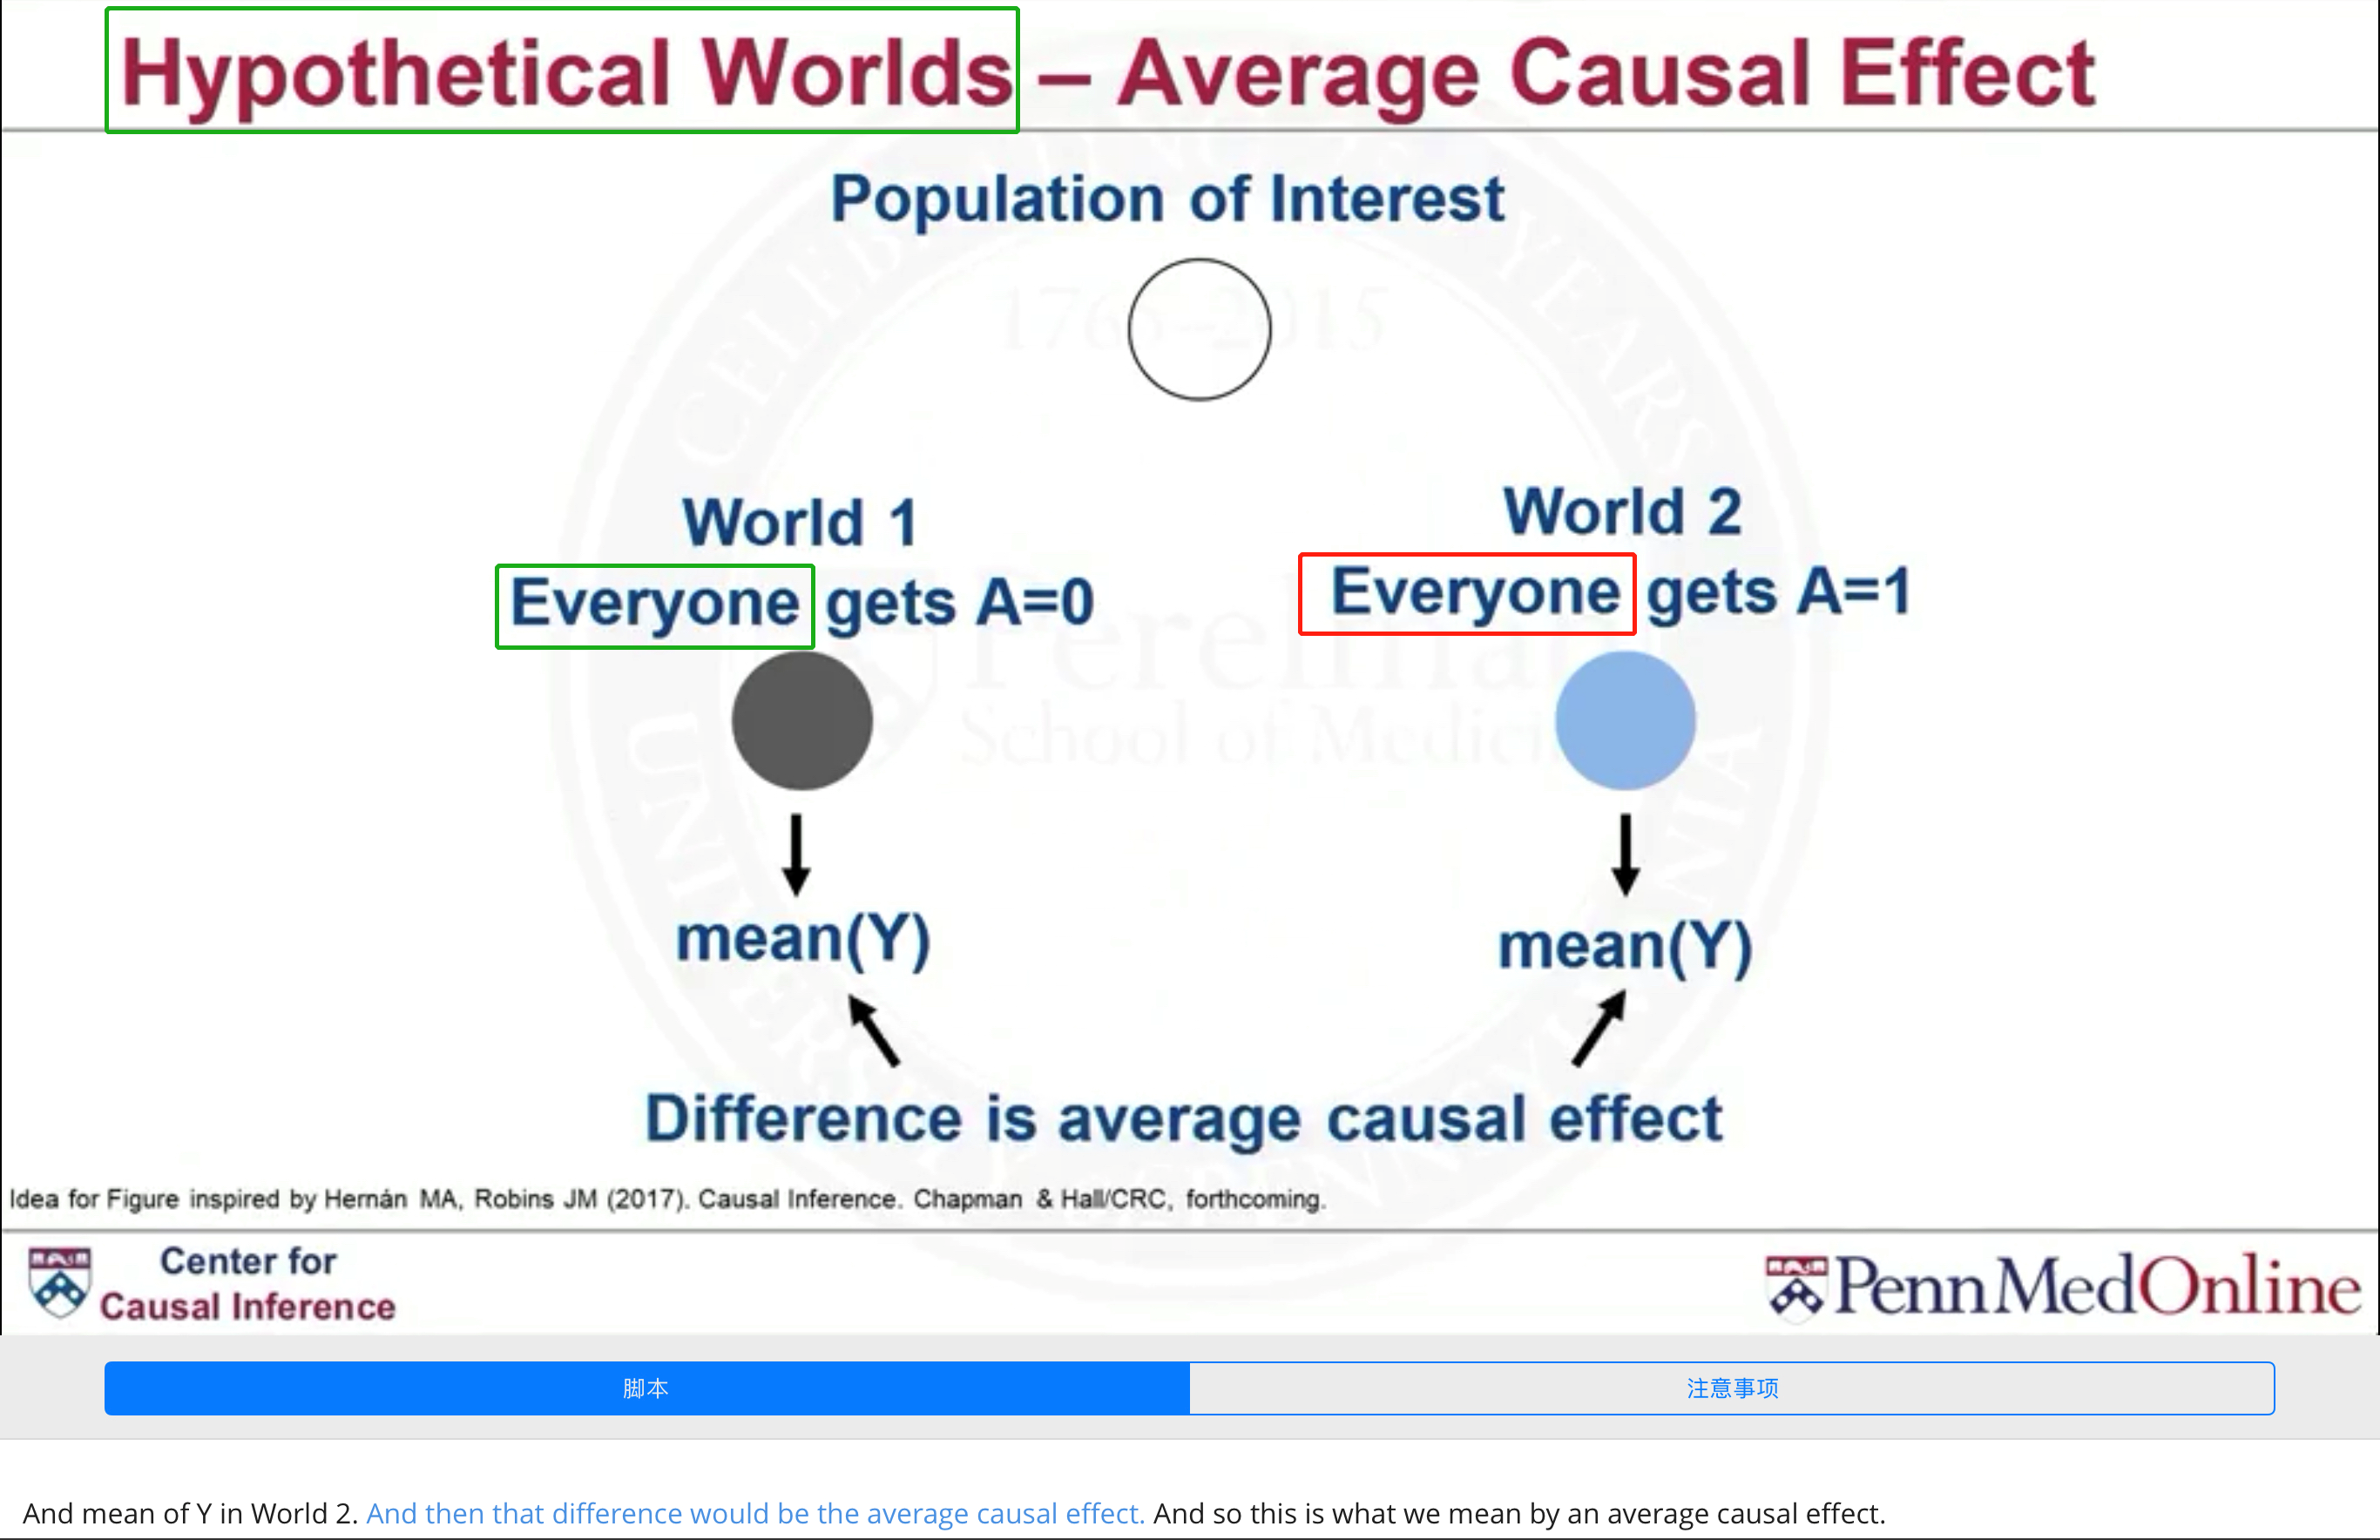
\includegraphics[width=0.7\textwidth]{figure/ACE.png}
	\caption{Average Causal Effect}
	\label{ACE}
\end{figure}

\subsection{Conditioning on versus setting}
这一部分主要是辨析概念:
\begin{equation}
E(Y^1-Y^0) \neq E[Y|A=1]- E[Y|A=0]
\end{equation}
\begin{itemize}[itemindent = 0em]
    \item[$\blacktriangleright$]$E(Y^1-Y^0)$是whole population都进行处理$A=1$与whole population都进行处理$A=0$时average outcome的差值. 
    \item[$\blacktriangleright$]$E[Y|A=a]$是在给定$A=a$的情况下$Y$的均值,相当于在$A=a$的这部分人中求average outcome. 于是$E[Y|A=1]-E[Y|A=0]$表示$A=1$的这部分人与$A=0$的另一部分人的average outcome的差值.
\end{itemize}

对象从population变成了subpopulation. 所以两者本质是不一样的:
\begin{itemize}[itemindent = 2em]
	\item Setting(manipulating) treatment $\Longrightarrow$ potential outcome situation.
    \item Conditioning on $\Longrightarrow$ restricting to subpopulation.
\end{itemize}

slides如Fig.\ref{versus}所示.
\begin{figure}[htbp]
	\setlength{\abovecaptionskip}{0pt}     %调整图片标题与图距离
	\setlength{\belowcaptionskip}{10pt}
	\vspace{-0cm}  %调整图片与上文的垂直距离
	\setlength{\abovecaptionskip}{-0cm}   %调整图片标题与图距离
	\setlength{\belowcaptionskip}{0cm}   %调整图片标题与下文距离
	\centering
	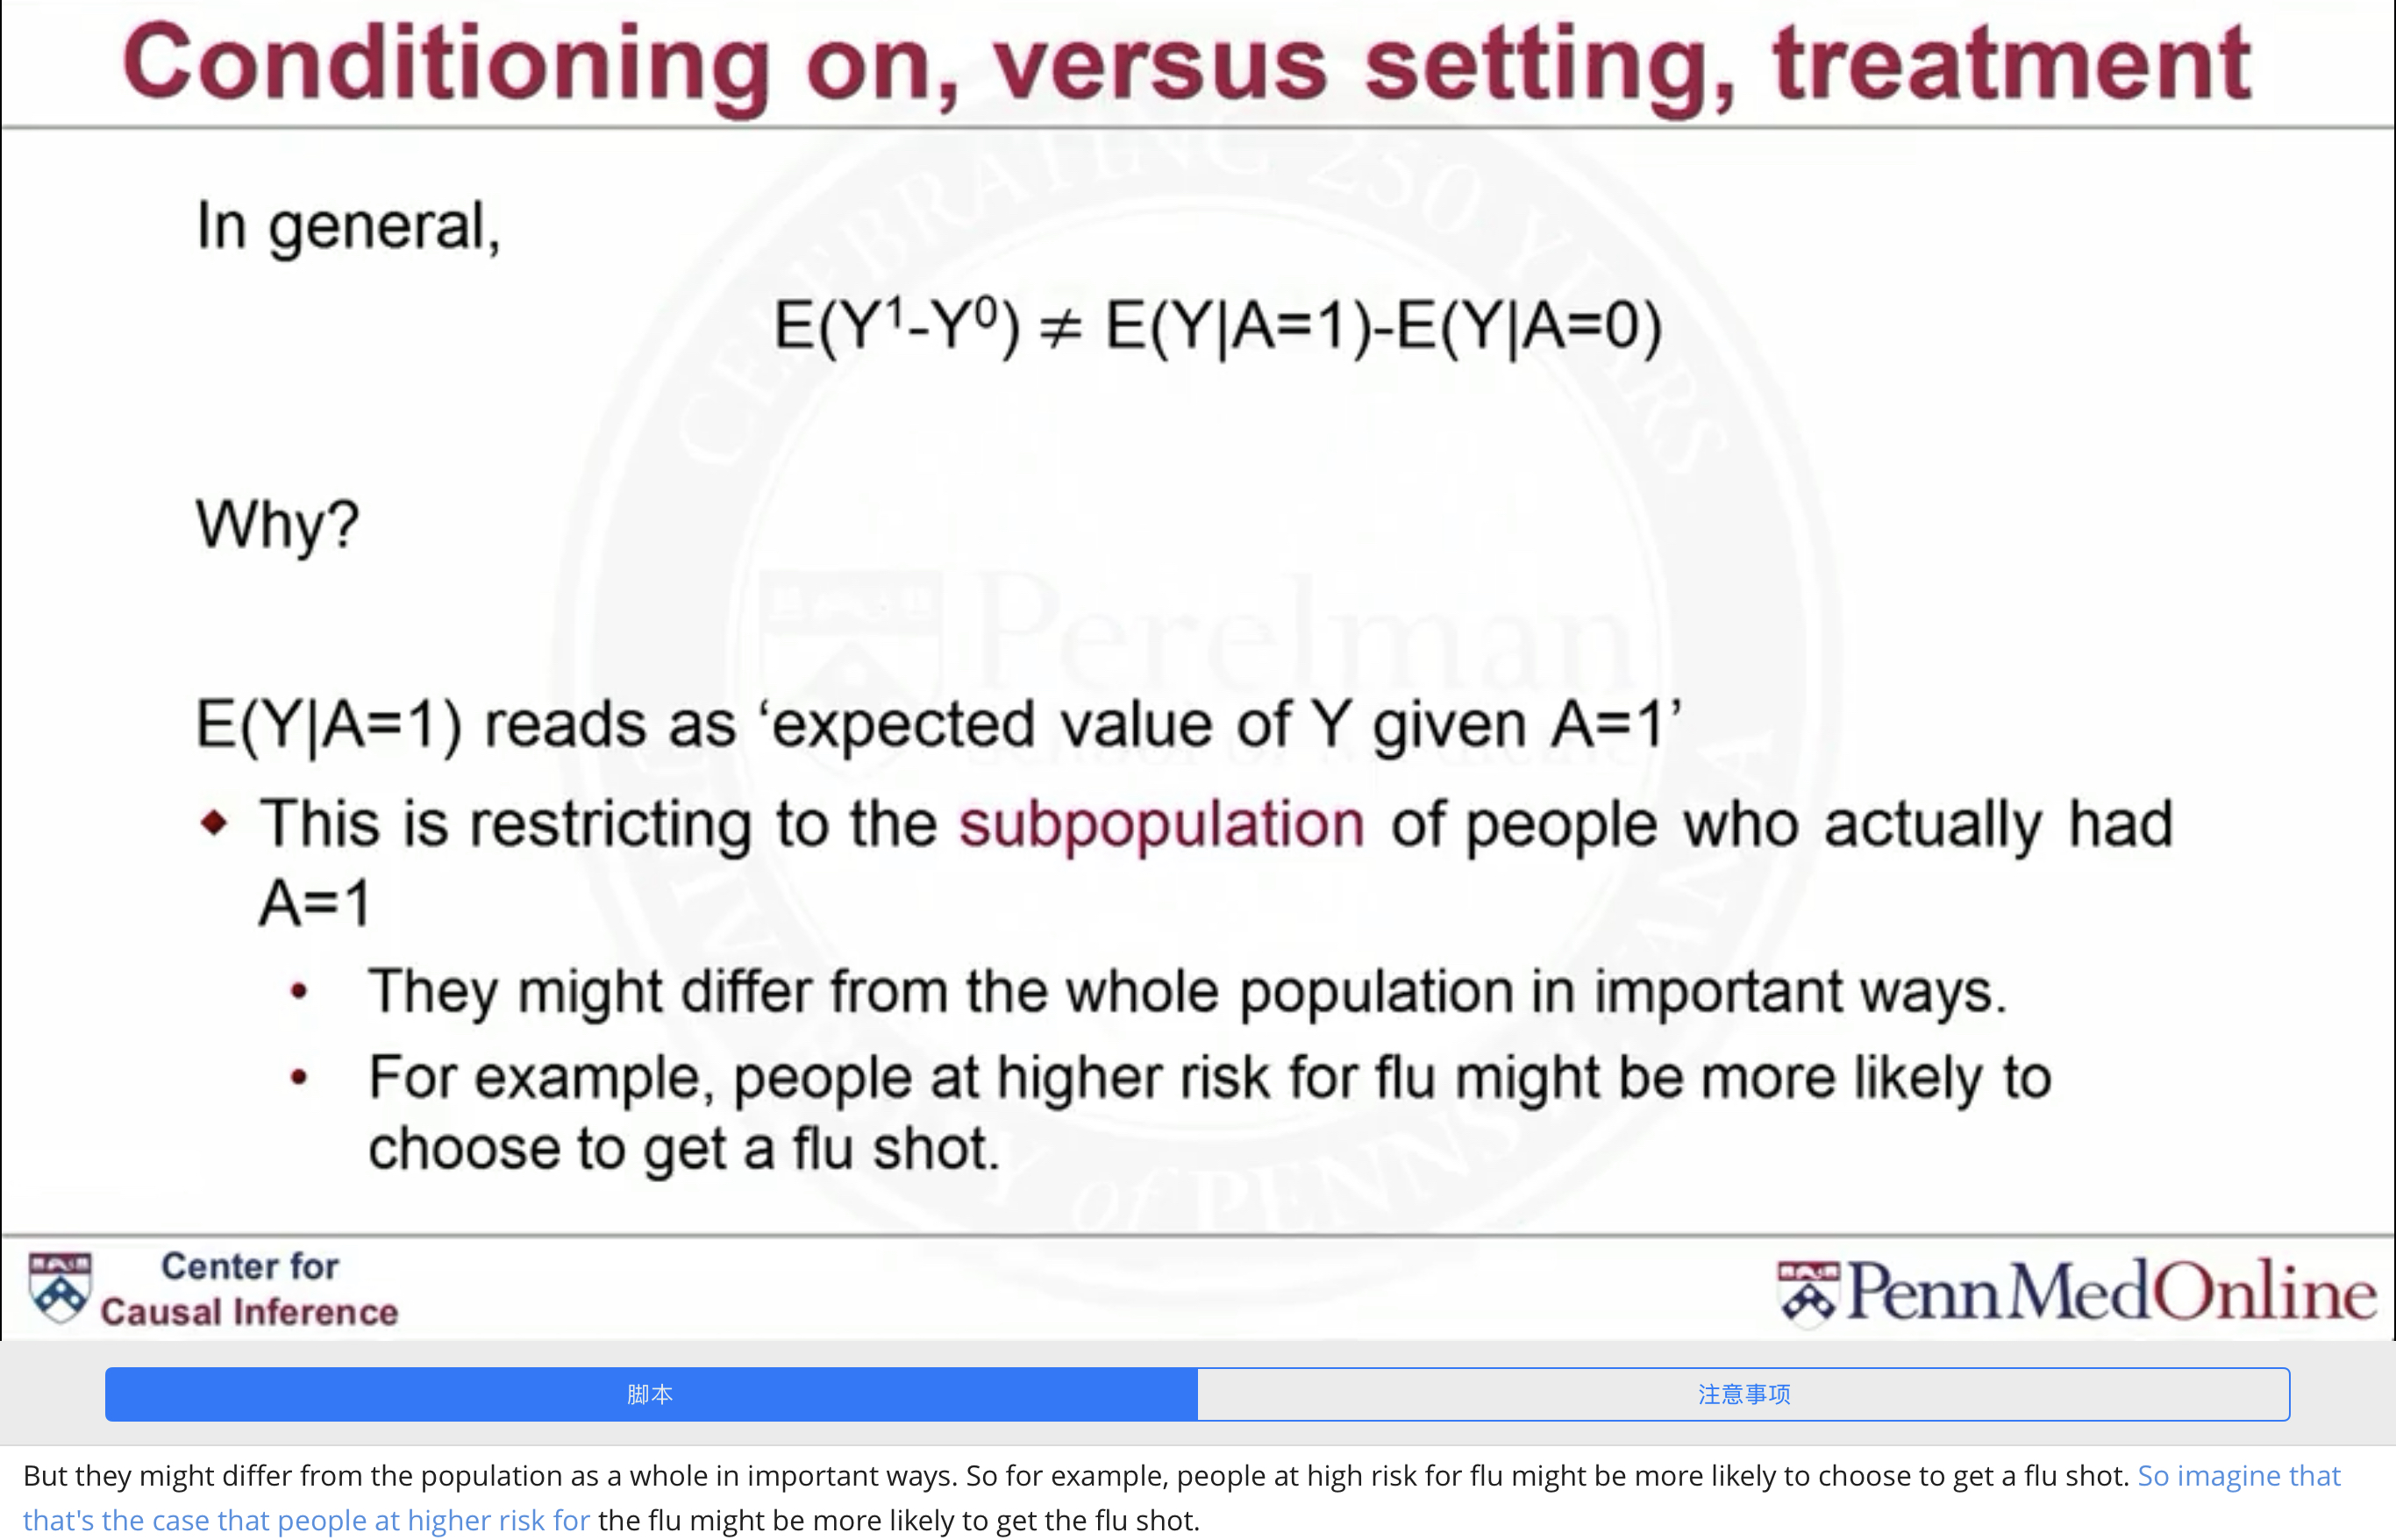
\includegraphics[width=0.8\textwidth]{figure/versus.jpg}
	\caption{Conditioning on,versus setting,treatment}
	\label{versus}
\end{figure}
	
\subsection{The definition of "the causal effect of treatment on the treated"}
这个概念是针对subpopulation来说的. 直接看slides就能明白,如Fig.\ref{CETT}.
\begin{figure}[htbp]
	\setlength{\abovecaptionskip}{0pt}     %调整图片标题与图距离
	\setlength{\belowcaptionskip}{10pt}
	\vspace{-0cm}  %调整图片与上文的垂直距离
	\setlength{\abovecaptionskip}{-0cm}   %调整图片标题与图距离
	\setlength{\belowcaptionskip}{-0cm}   %调整图片标题与下文距离
	\centering
	
\includegraphics[width=0.8\textwidth]{figure/CETT.png}
	\caption{The causal effect of treatment on the treated}
	\label{CETT}
\end{figure}

\subsection{Conclusion}
从这一课中我们学到了非常重要的概念辨析. 什么是causal effect?为什么条件均值差$E[Y|A=1]-E[Y|A=0]$不能作为causal effect?
这些概念的重点在于区分{\color{red}treatment是针对whole population还是whole population中的不同subpopulation. }
Causal effect之所以是Causal effect,是因为它针对的是整个population的潜在结果差异. 现实中不可度量. 而其他条件均值差之所以不能作为Causal effect,是因为它针对的是different people的结果差异.
这一点非常重要. 以一张图可以总结这一课的重点:
\begin{figure}[htbp]
	\setlength{\abovecaptionskip}{0pt}     %调整图片标题与图距离
	\setlength{\belowcaptionskip}{10pt}
	\vspace{-0cm}  %调整图片与上文的垂直距离
	\setlength{\abovecaptionskip}{-0cm}   %调整图片标题与图距离
	\setlength{\belowcaptionskip}{-0cm}   %调整图片标题与下文距离
	\centering
	\includegraphics[width=0.8\textwidth]{figure/ConditionVSsetting.png}
	\caption{Conditioning Versus setting}
	\label{ConditionVSsetting}
\end{figure}

% 第一章新课时 
\newpage \section{Causal Assumptions} \label{Causal assumption}
\noindent {\bfseries Outline}:
\begin{itemize}
	\item[$\blacktriangleright$] Identifiability
	\item[$\blacktriangleright$] SUTVE 
	\item[$\blacktriangleright$] Consistency assumption
    \item[$\blacktriangleright$] Ignorability assumption
    \item[$\blacktriangleright$] Positivity assumption
\end{itemize}

\subsection{Identifiability}
Statistical identifiability: If a parameter can be estimated from actual data, it is considered identifiable.

{\color{red} Identifiability of causal effect} requires making some {\color{red} untestable} assumptions.
Assumptions will be about the observed data:$Y,A,X$.
假设是为了让我们能够从观测数据中识别Causal effect,因为实际上causal effect是不可观测的,所以估计causal effect需要加一些假设. 
\subsection{Stable Unit Treatment Value Assumption}
SUTVA的含义分为两层,No inference and one version of treatment.\\
\noindent (1) {\color{red} No inference:}
\begin{enumerate}[labelindent=2\parindent, leftmargin=*,align=left,widest=IV,label=\Roman*.]
	\item 每个受试者之间没有相互影响.
	\item 一个受试者的处理分配不会影响其他受试者的outcome. 
\end{enumerate}

这意味着每个受试者的outcome与其他人是无关的.\\

\noindent(2) {\color{red} One version of treatment:}

There is one variable that we can hypothetically intervene on and it's very well defined what we mean by treatment.
这一部分的作用是使得treatment的意义更加明确,假设我们干预了某个variale,并且这个variable就是我们定义的treatment.

SUTVA的作用就是“我们可以把第$i$个受试者的potential outcome” 表示成其自身所接受的treatment的形式. 而不受其他受试者的影响.

\subsection{Consistency Assumption}
The potential outcome under treatment $A=a: Y^a$ is equal to the observed outcome $Y$ if the actual treatment received is $A=a$.
\begin{equation}
\text{observed outcome  }Y = Y^a,\quad \text{if A=a, for all a.}
\end{equation} 
这则假设告诉我们,真实处理$A=a$下的观测结果$Y$可以看做接受处理$A=a$时的potential outcome.

\subsection{Ignorability assumption}
Given pre-treatment covariates $X$, treatment assignment is independent from the potential outcomes. Or Potential outcomes are independent of treatment assignment conditional on covariates X.
\begin{equation}
Y^0,Y^1 \perp A|X.
\end{equation}
这则假设说明在给定$X$后,对于$X$取值相同的受试者来说,处理$A$的分配是随机的. Potential outcome与处理的分配无关. 

此外,Ignorability assumption还有两个别称:
\begin{enumerate}[label=(\arabic*)]
	\item Conditional independence assumption(CIA):Conditioning on $X$,$Y^0, Y^1$与$A$独立. 
    \item No unmeasured confounders, 指所有的confounders都被measure到,控制了这些confounders就可以把$A$看做是随机分配的.
\end{enumerate}


\subsection{Positivity Assumption}
For every set of values for $X$, treatment assignment was not deterministic:
\begin{equation}
P(A=a|X=x)>0,\text{  for all a and x.}
\end{equation} 

这则假设说明:对于给定的$X$,每个个体都有可能接受任何处理. 如果某个个体不可能接受another treatment,也就意味着我们不能观测到他的potential outcome. 这就违背了causal effect的本质.

\subsection{Observed Data and Potential Outcomes}
结合上述4条假设,是通过observed data识别causal effect的基础. 实现从$E(Y|A=a,X=x)$到$E(Y^a|X=x)$的转化. Fig.\ref{assump}很好地说明了assumptions在因果推断中的作用.
\begin{figure}[htbp]
	\setlength{\abovecaptionskip}{0pt}     %调整图片标题与图距离
	\setlength{\belowcaptionskip}{10pt}
	\vspace{-0cm}  %调整图片与上文的垂直距离
	\setlength{\abovecaptionskip}{-0cm}   %调整图片标题与图距离
	\setlength{\belowcaptionskip}{-0cm}   %调整图片标题与下文距离
	\centering
	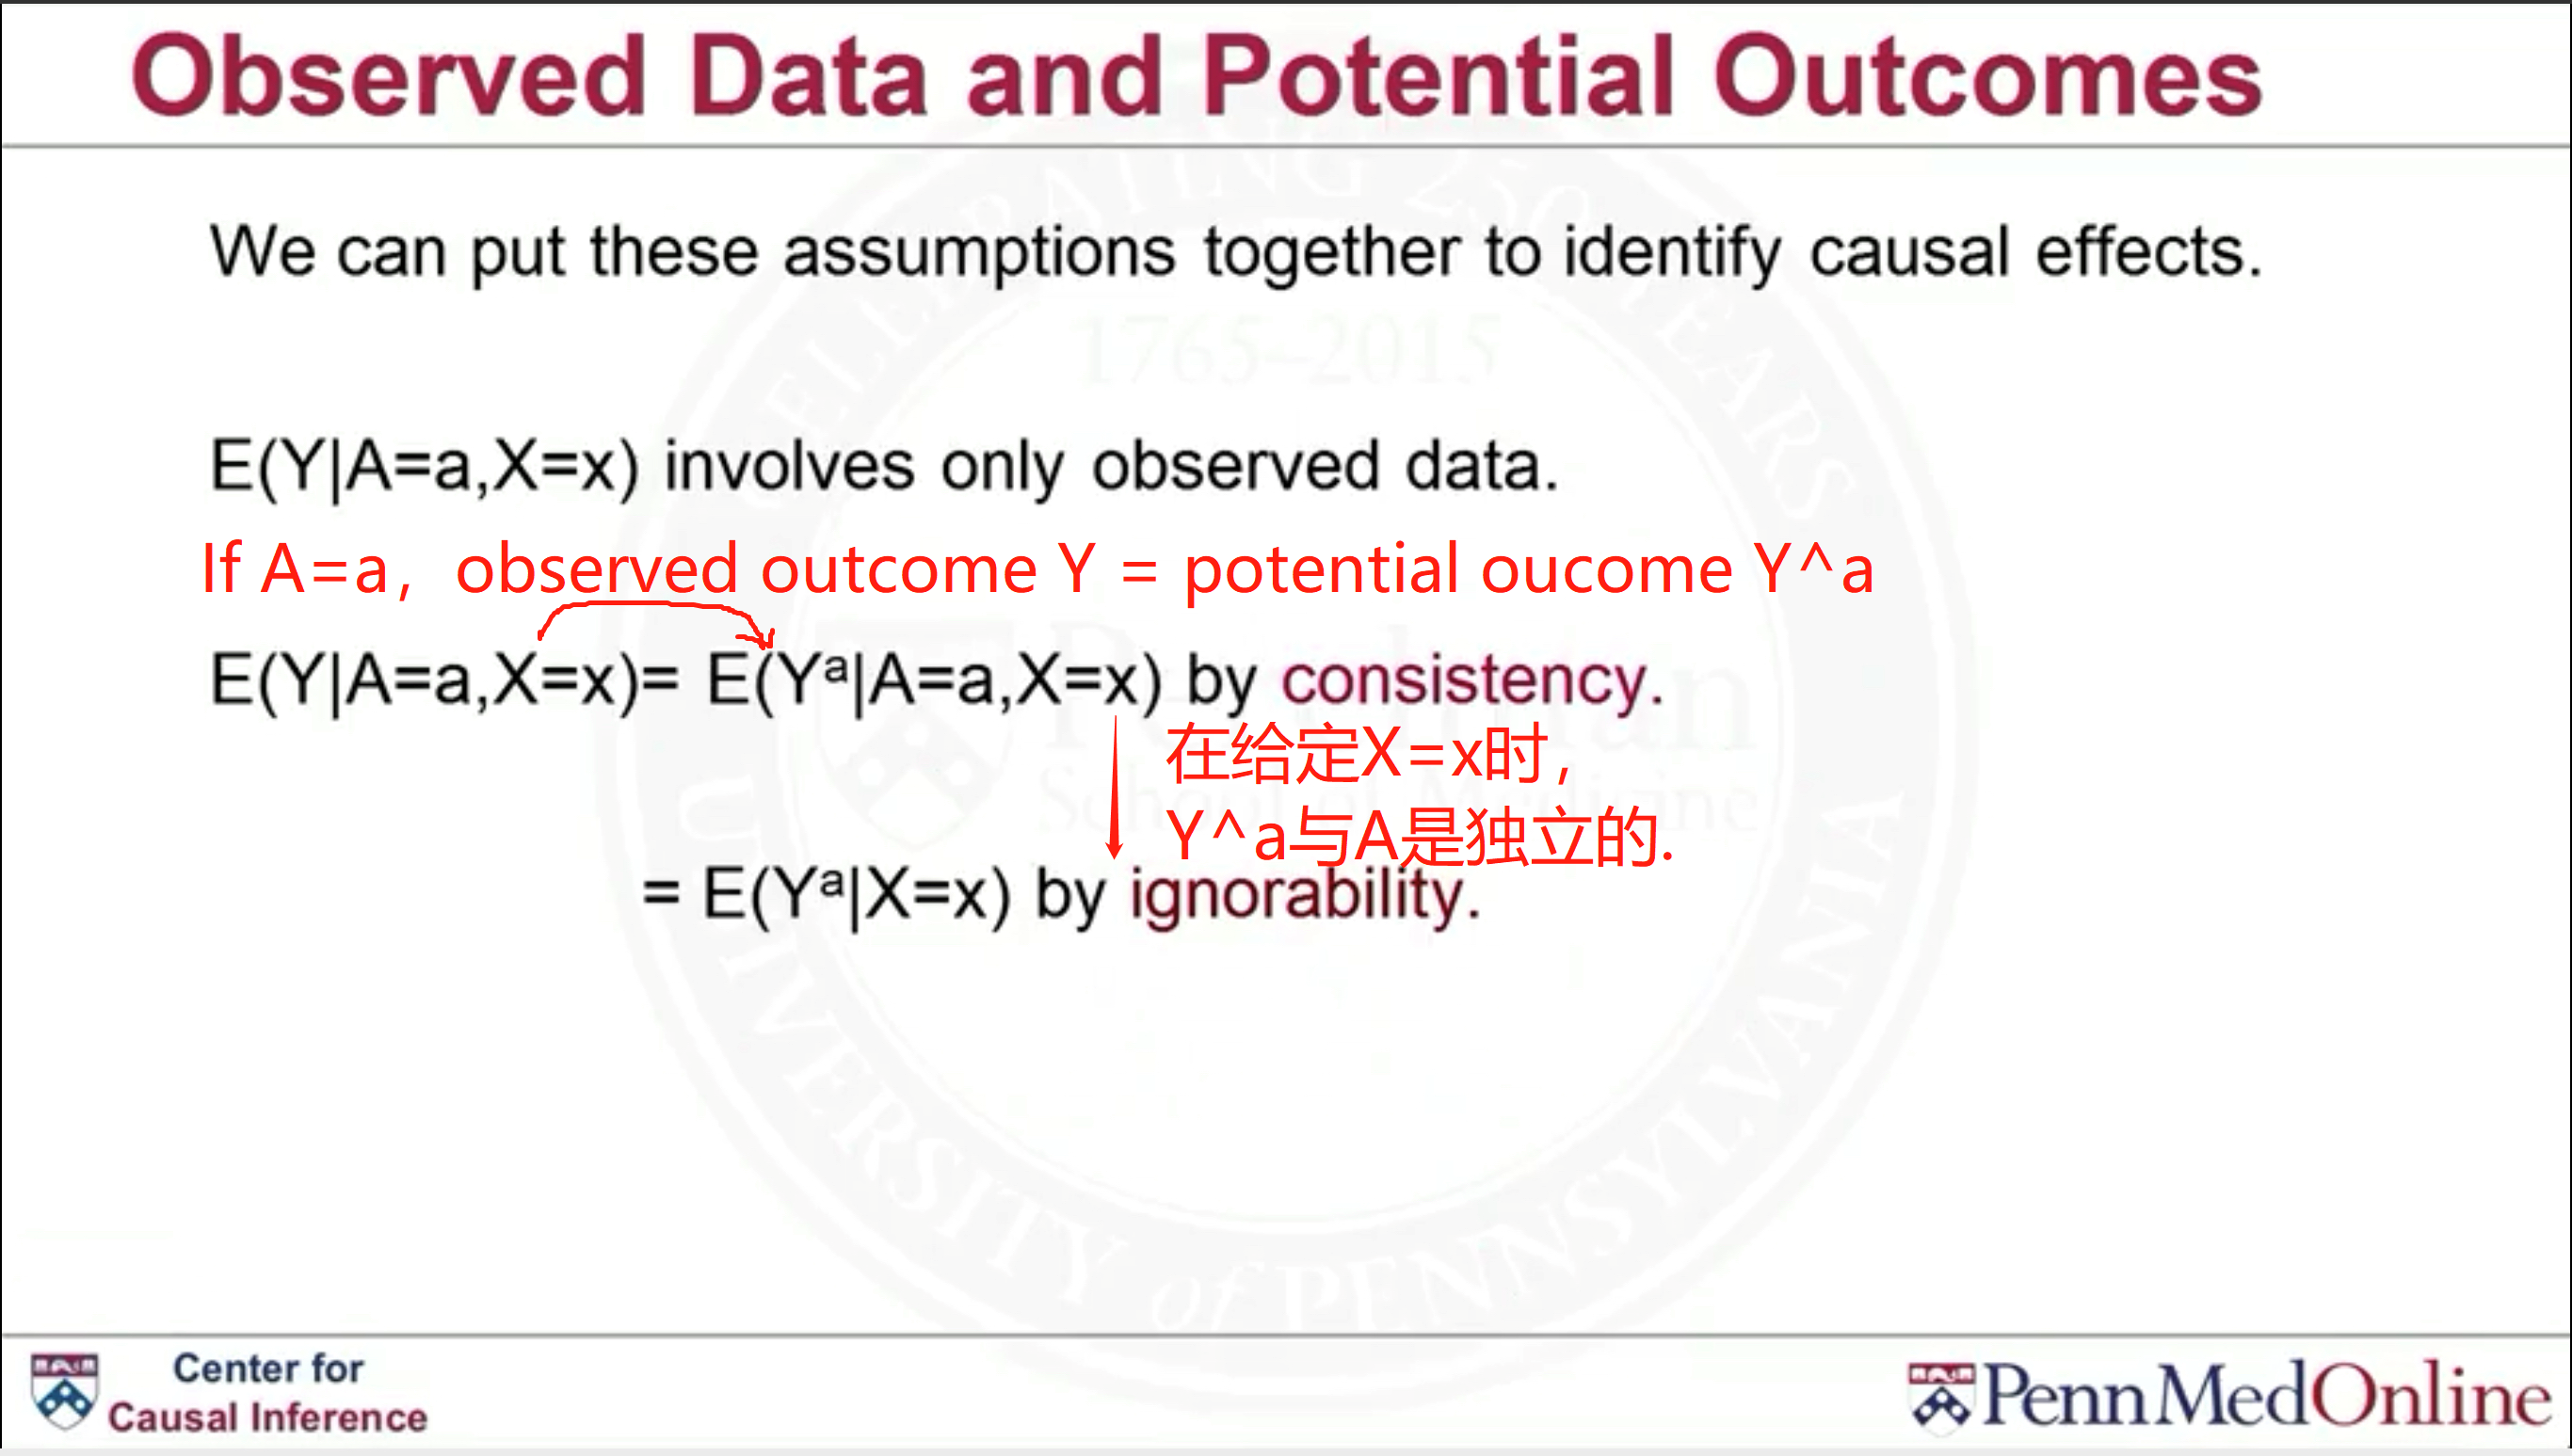
\includegraphics[width=0.8\textwidth]{figure/assump.png}
	\caption{Observed Data and Potential Outcomes}
	\label{assump}
\end{figure}

\newpage \section{Stratification}
这一部分讲了估计causal effect的一种简单思想,但只适用于非常简单的情形,因此几乎没有实际应用.

在第\ref{Causal assumption}节中,我们已经知道通过假设可以实现
\begin{equation}
E(Y|A=a,X=x)=E(Y^a|X=x)
\end{equation}
那么potential outcome的均值就可以通过遍历$X$的取值求得:
\begin{equation}
E(Y^a)=\sum_{x} E(Y^a|X=x)P(X=x) =\sum_{x} E(Y|A=a,X=x)P(X=x)
\end{equation}
称$E(Y^a)$为standardized mean. 

Standardization包含了"stratifying"和"averaging"两层结构.
我们可以将所有样本按照$X$和$A$分层,然后分别求出在不同的$X$和$A$下outcome的均值.下面用一个例子说明Stratification的用法. 
\begin{ex}
某机构正在研究两种药物:saxagliptin(简称saxa)和sitagliptin(简称sita)对主流心脏病发病(MACE)的影响. 口服抗糖尿病药物(oral antidiabetic drug,简称OAD)是协变量. 已知选择药物saxagliptin治疗的病人之前多服用过OAD,而服用OAD的病人有更高的患MACE的风险.
\end{ex}

现在我们整理一下解题思路:\\
\begin{figure}[htbp]
	\setlength{\abovecaptionskip}{0pt}     %调整图片标题与图距离
	\setlength{\belowcaptionskip}{10pt}
	\vspace{-0cm}  %调整图片与上文的垂直距离
	\setlength{\abovecaptionskip}{-0cm}   %调整图片标题与图距离
	\setlength{\belowcaptionskip}{-0cm}   %调整图片标题与下文距离
	\centering
	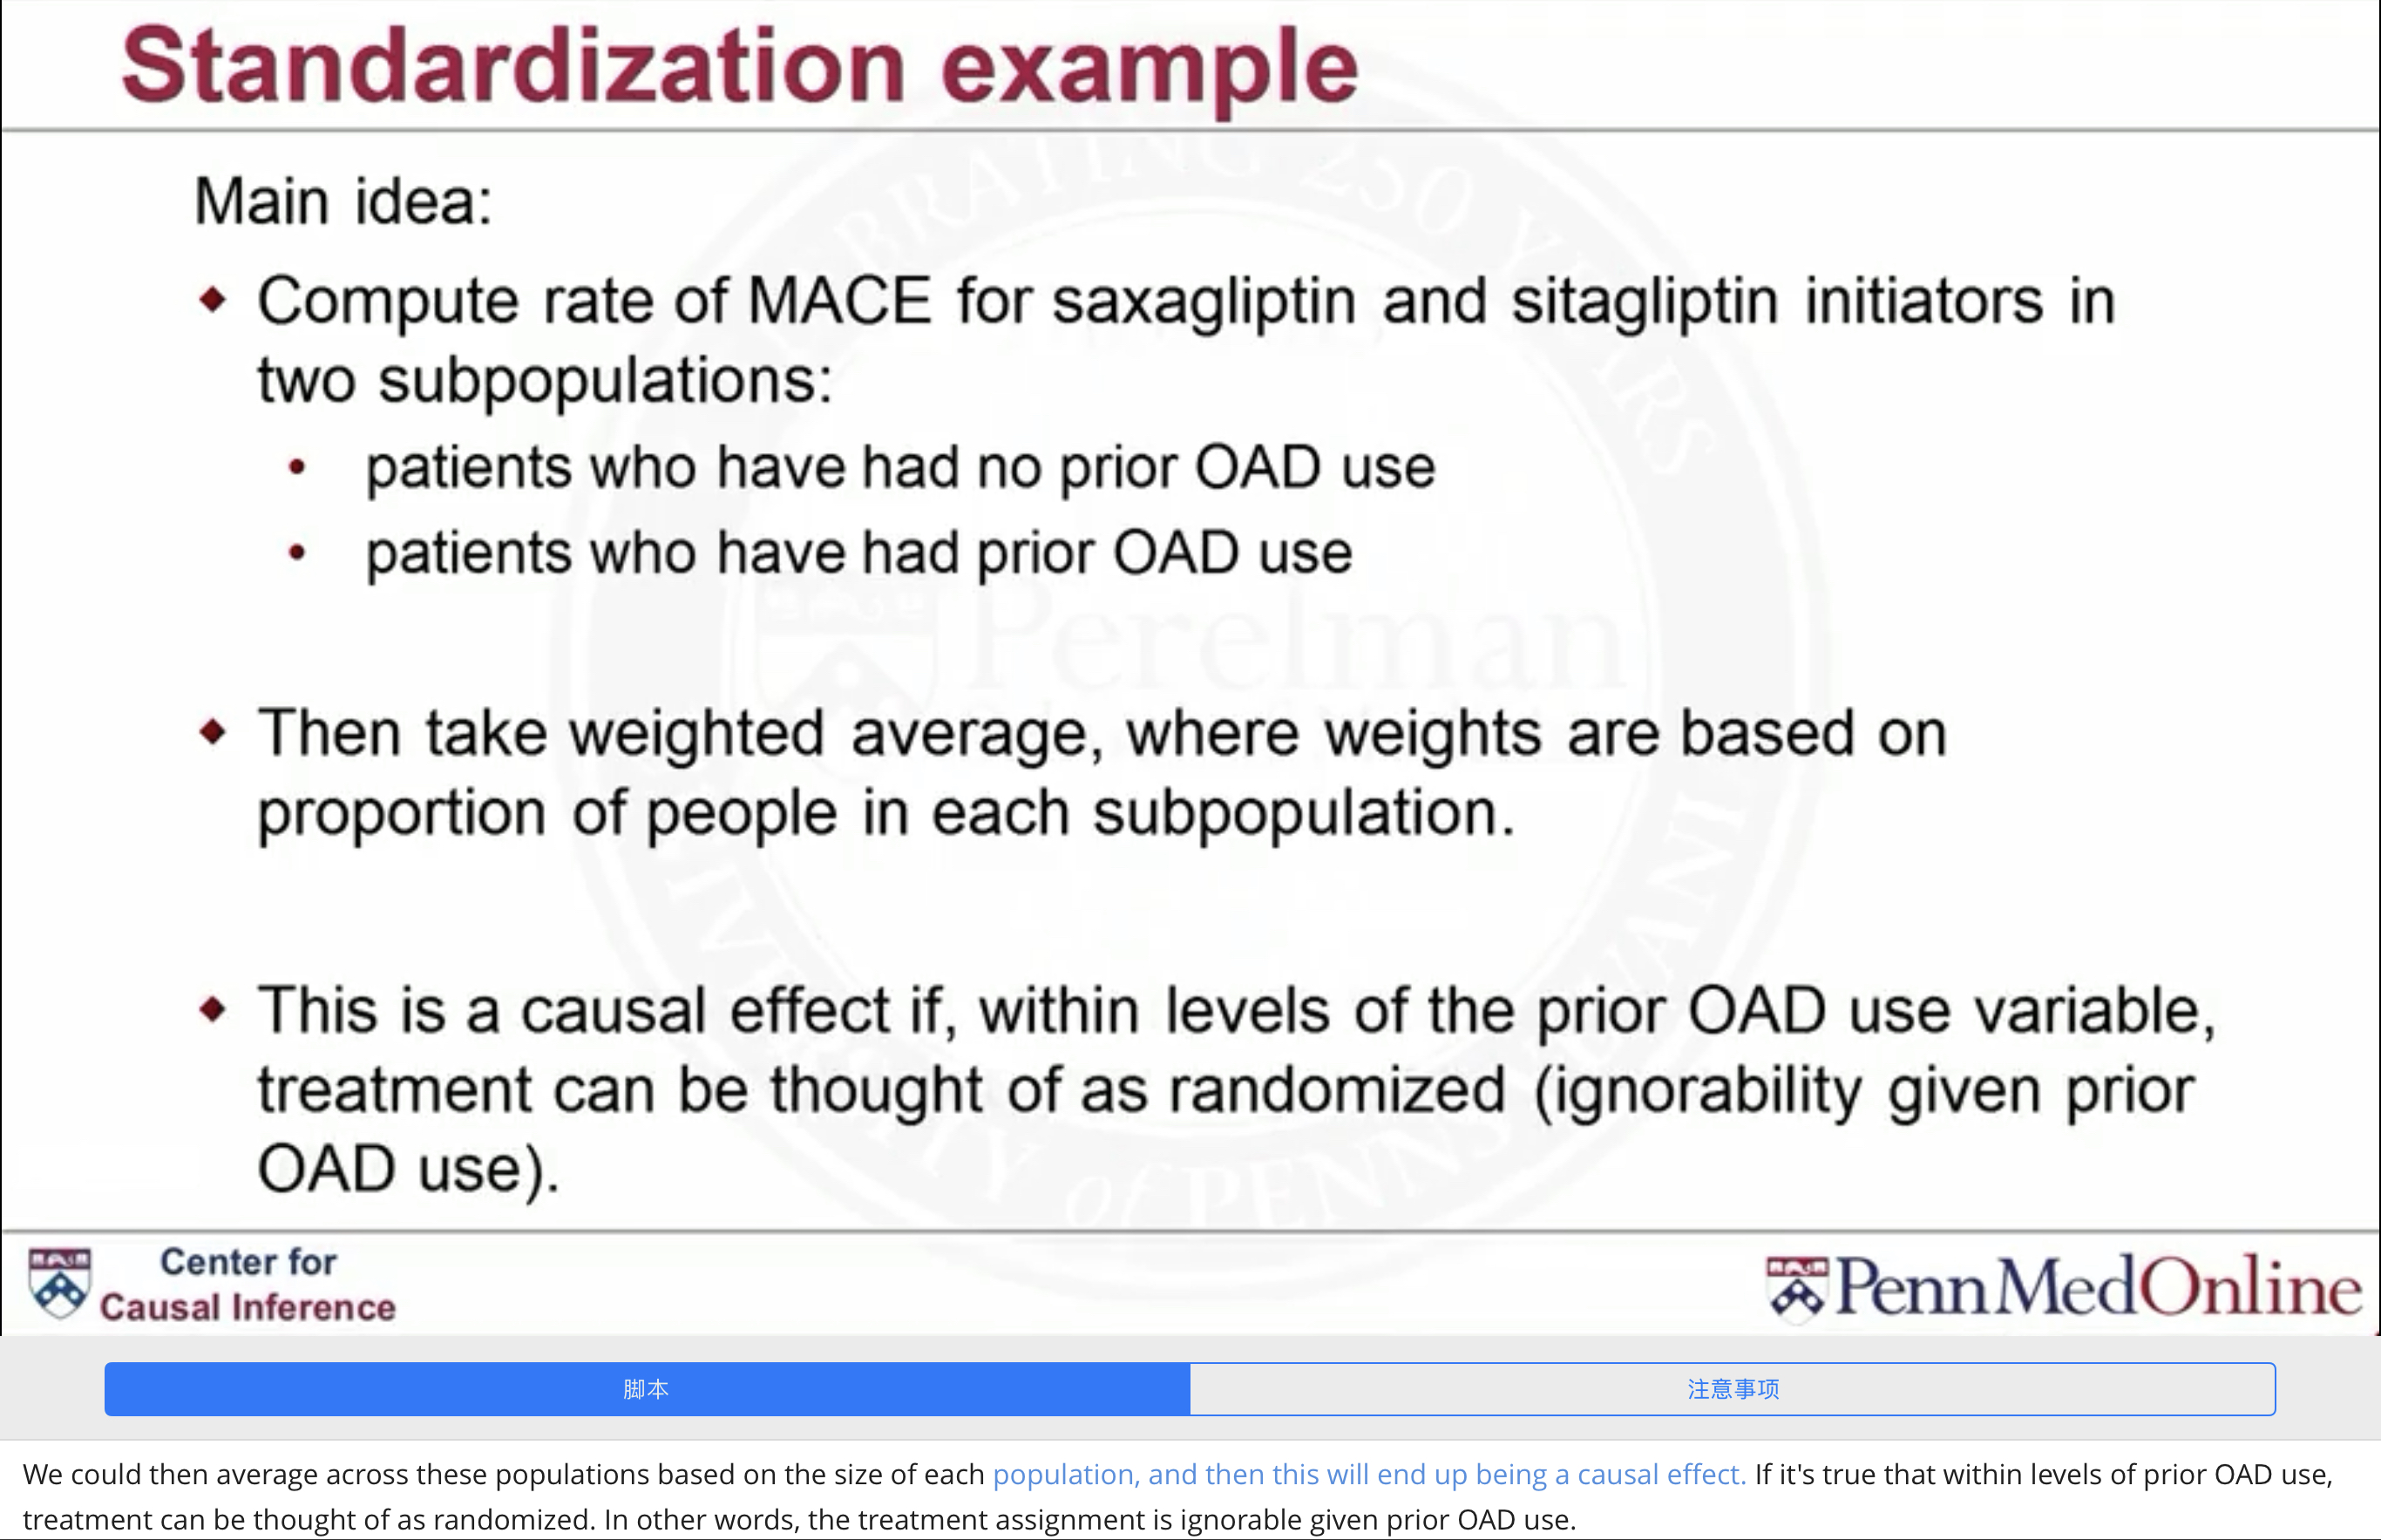
\includegraphics[width=0.8\textwidth]{figure/strtidea.jpg}
	\caption{Main idea of Stratification}
	\label{strtidea}
\end{figure}

接下来要做的就是按照$X$将数据分层:服用过OAD的分为一组,在whole population中所占的比例记为P(prior OAD use yes);未服用过OAD的分成另一组,所占比例记为P(prior OAD use no). 

在每一组中再按照$A$的取值划分层次:$A=saxa$划为一层,$A=sita$的划为另一层. 共得到4层样本,然后在每一层上计算患MACE的比例. 计算的过程如Fig.\ref{meansaxa}和Fig.\ref{meansita}所示.
    \begin{figure}[htbp]
	%\setlength{\abovecaptionskip}{0pt}     %调整图片标题与图距离
	%\setlength{\belowcaptionskip}{10pt}
	\vspace{-0cm}  %调整图片与上文的垂直距离
	\setlength{\abovecaptionskip}{0pt}   %调整图片标题与图距离
	\setlength{\belowcaptionskip}{2pt}   %调整图片标题与下文距离
	   \centering                                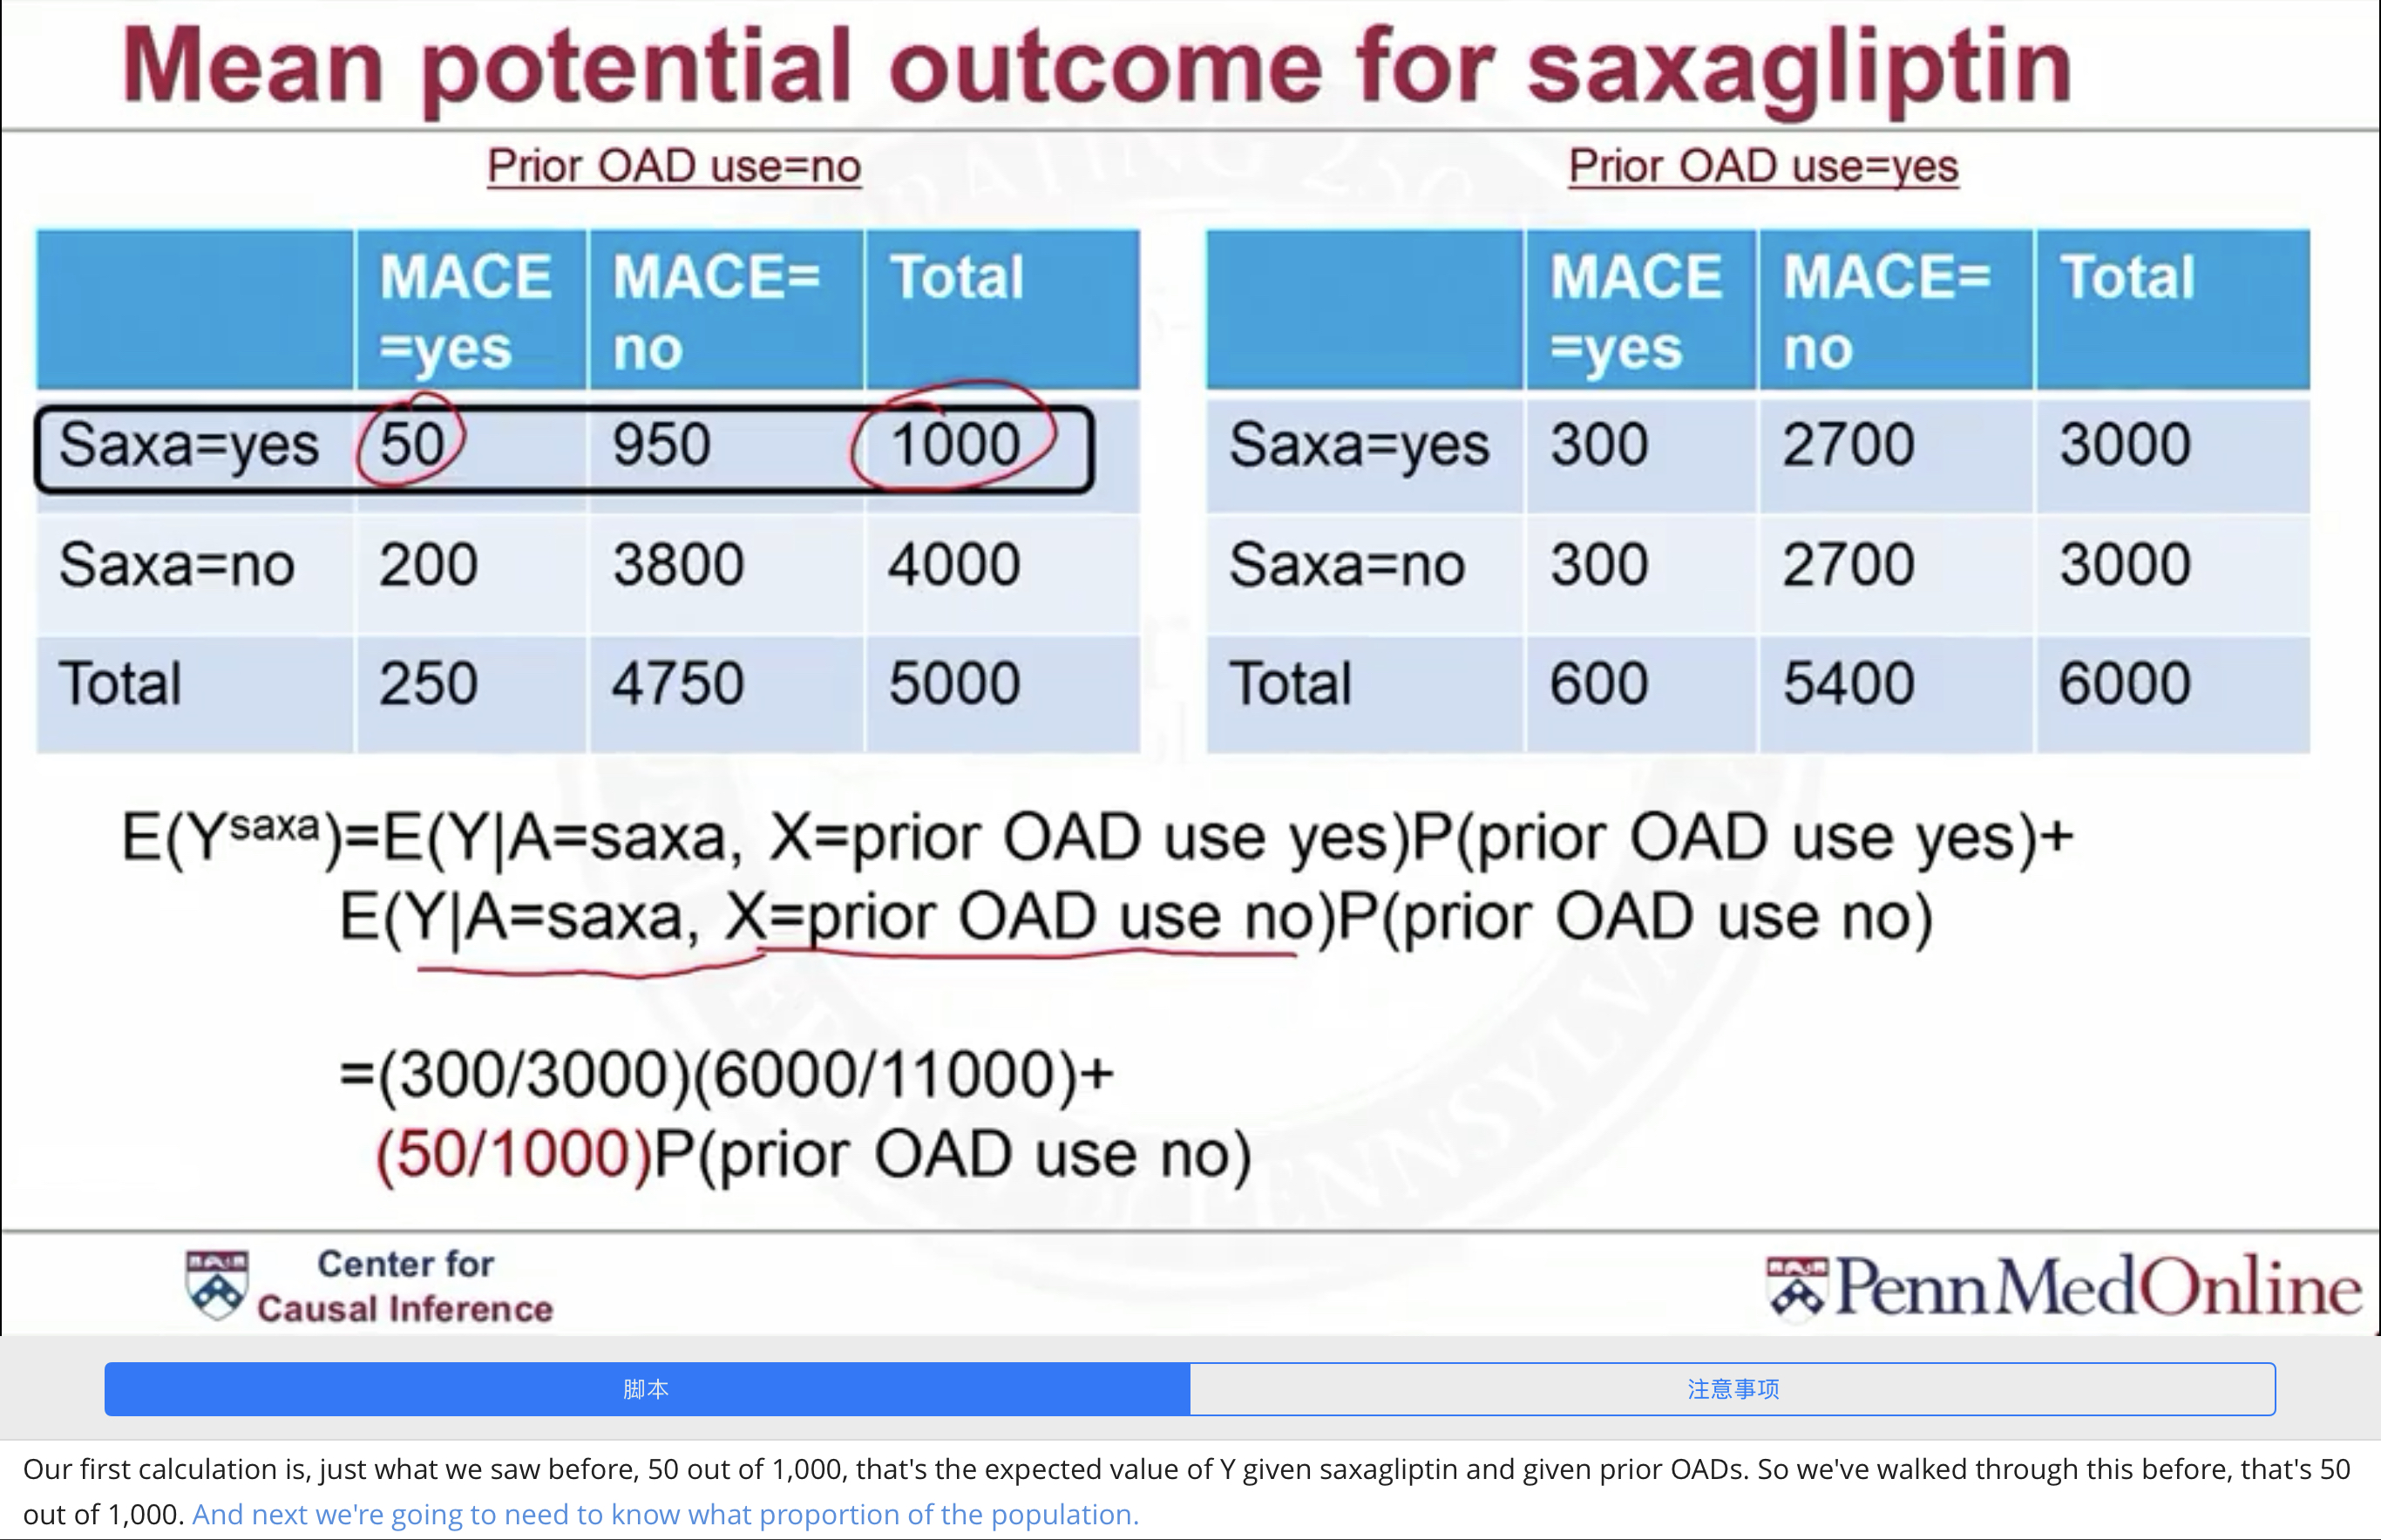
\includegraphics[width=0.8\textwidth]{figure/meansaxa.jpg}
	   \caption{Mean potential outcome for saxa}   
       \label{meansaxa}
       \end{figure}

	 \begin{figure}[htbp]
	 \setlength{\abovecaptionskip}{0pt}     %调整图片标题与图距离
	 \setlength{\belowcaptionskip}{10pt}
	 \vspace{-0cm}  %调整图片与上文的垂直距离
	 \setlength{\abovecaptionskip}{-0cm}   %调整图片标题与图距离
	 \setlength{\belowcaptionskip}{-0cm}   %调整图片标题与下文距离
	 \centering
     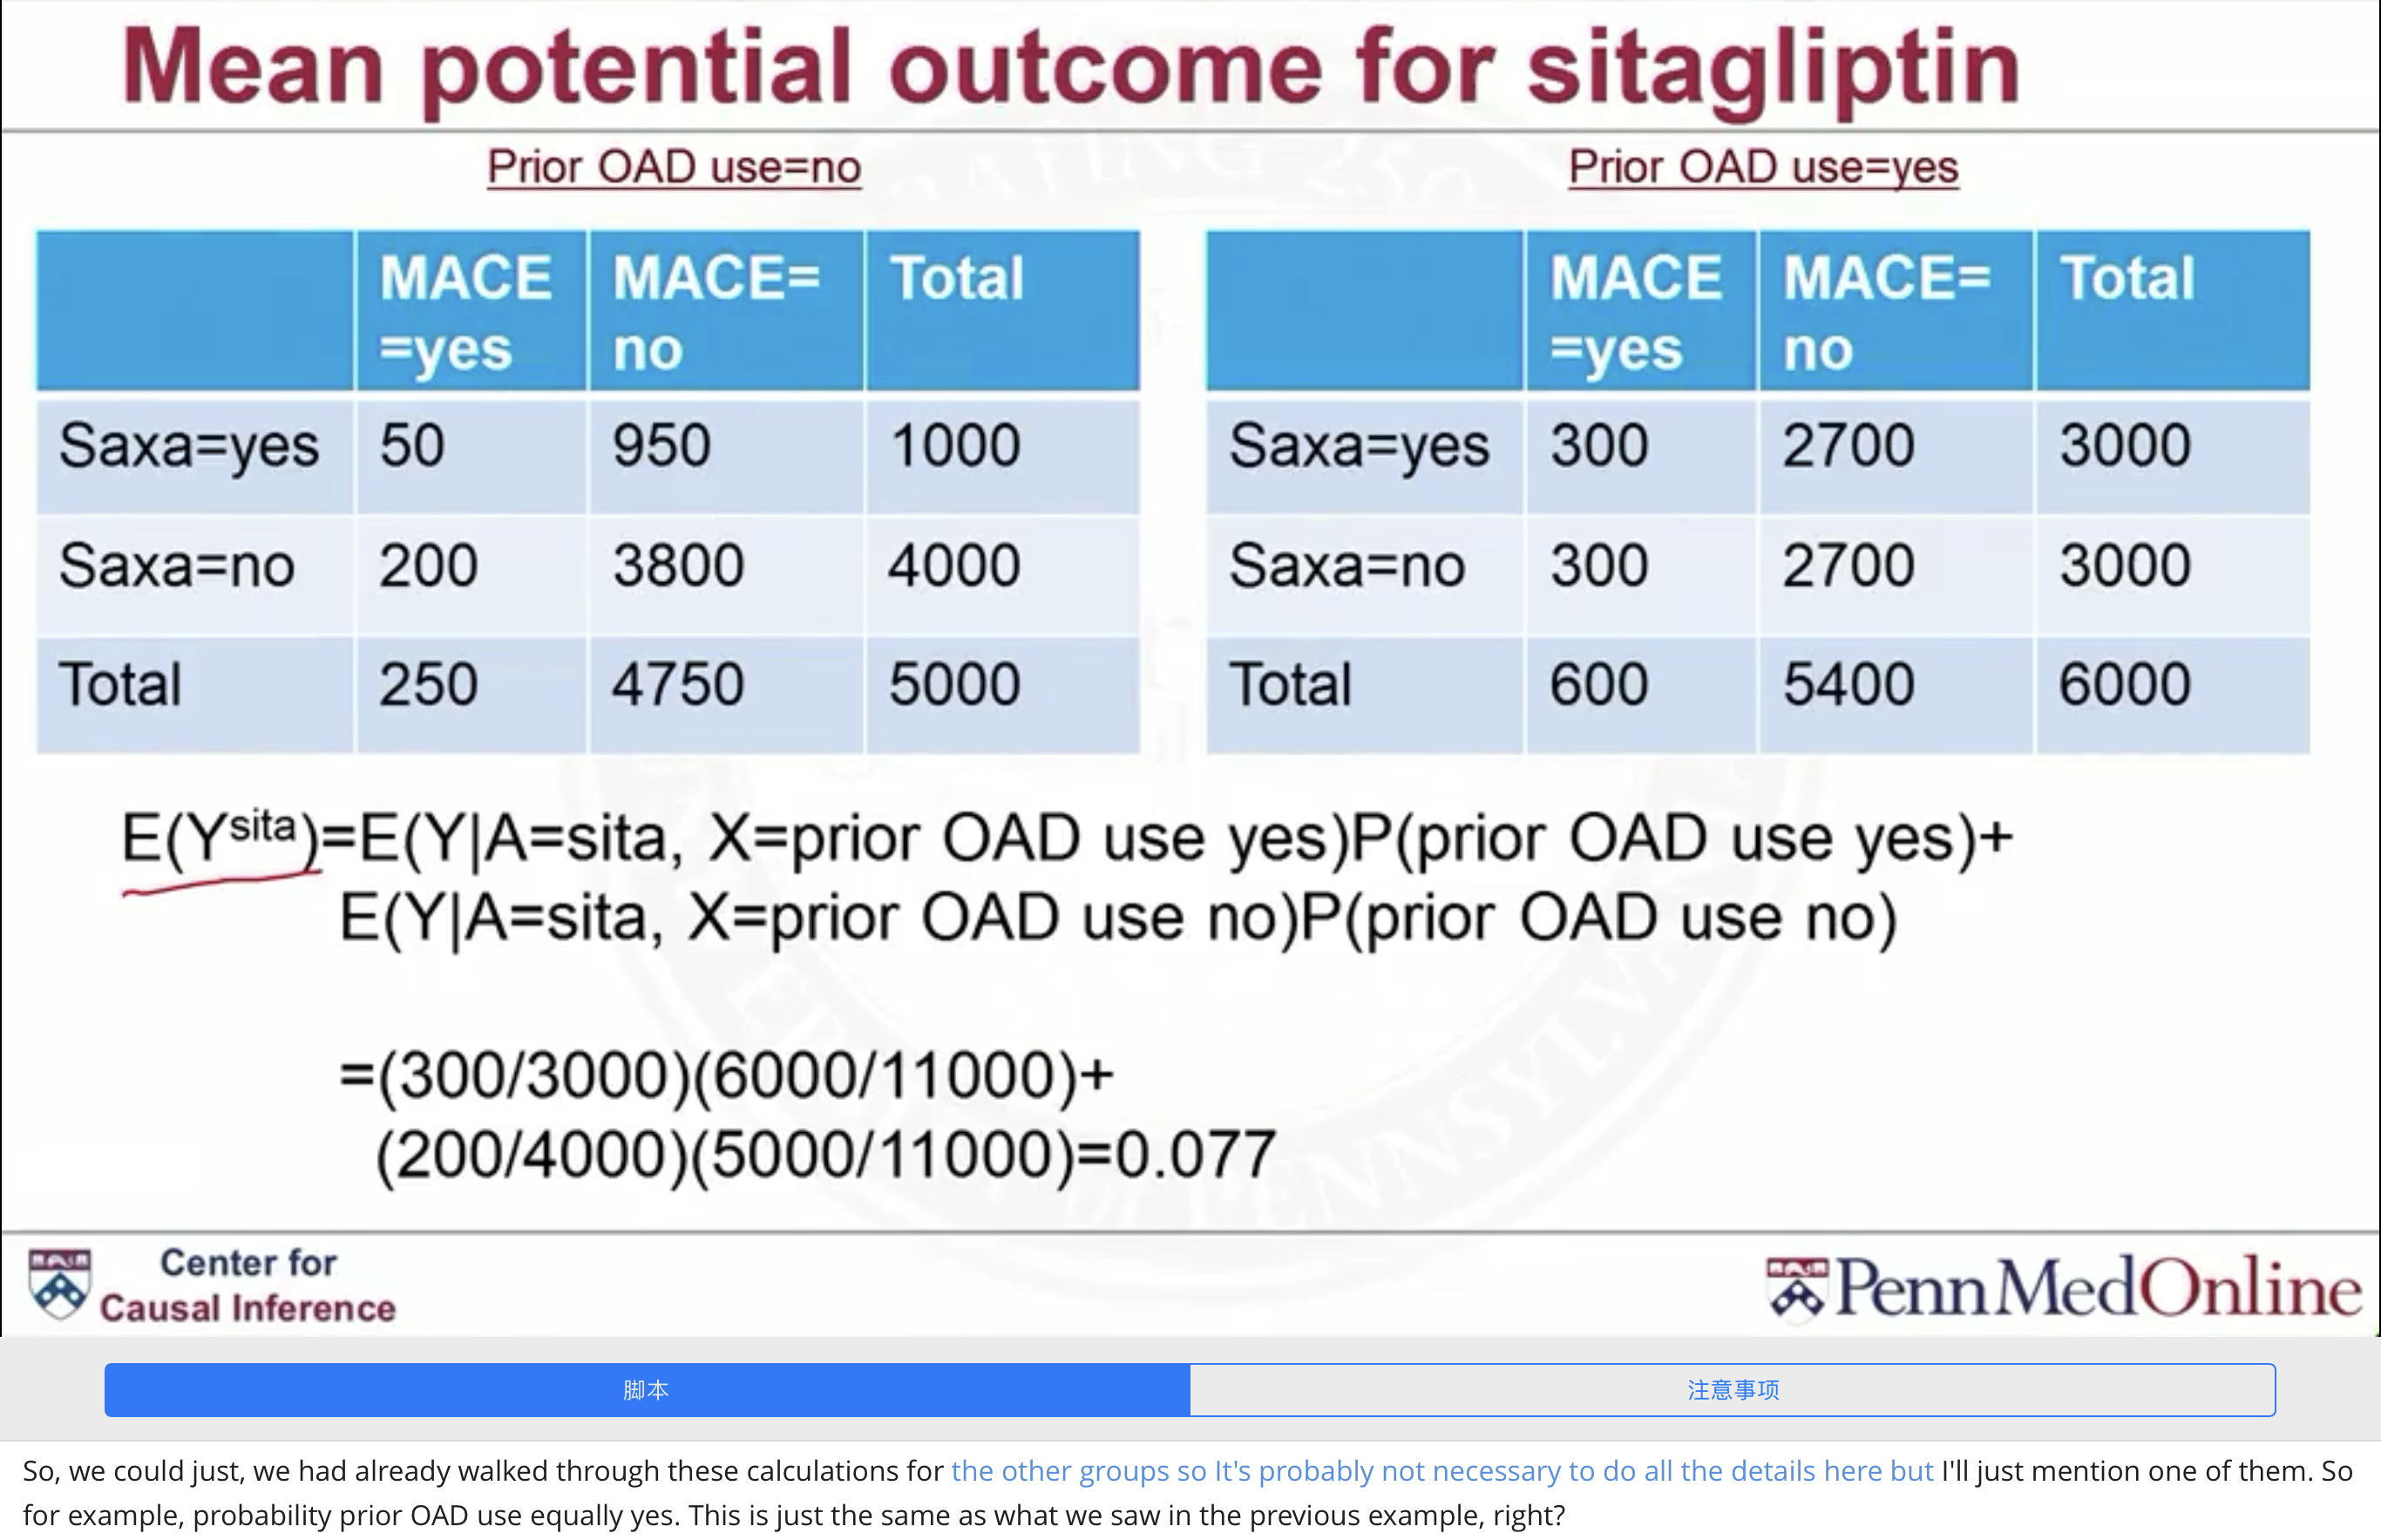
\includegraphics[width=0.8\textwidth]{figure/meansita.jpg} 
     \caption{Mean potential outcome for sita}
     \label{meansita}
     \end{figure}           
\subsection{Conclusion}
最后总结一下Stratification算法的缺陷:

\begin{figure}[h]
	\setlength{\abovecaptionskip}{0pt}     %调整图片标题与图距离
	\setlength{\belowcaptionskip}{10pt}
	\vspace{-0cm}  %调整图片与上文的垂直距离
	\setlength{\abovecaptionskip}{-0cm}   %调整图片标题与图距离
	%\setlength{\belowcaptionskip}{-0cm}   %调整图片标题与下文距离
	\centering
	
\includegraphics[width=0.8\textwidth]{figure/strtprm.jpg}
	\caption{Problems of Stratification}
	\label{strtprm}
\end{figure}

\newpage \section{Incident User and Active Comparator designs}
\noindent {\bfseries Outline:}\\
1. Two designs: Incident user design and active comparator designs.\\
2. Understand the basic idea of incident user design and what problem they help avoid.\\
3. Understand the basic idea of active comparator design and how they help to reduce confoundering.

\subsection{Cross-sectional look at treatments}
Suppose that we are interested in the causal effect of $A$ on the outcome $Y$. And we have a population of people, some of them are doing $A=1$, while some are not. Now suppose $A=$wheter regularly practicing yoga and $Y=$blood pressure. 

\paragraph{There are problems:} At any given time, some people regularly practice yoga while others not.
\begin{itemize}
	\item Those who do not might have in the past.
	\item Those who do might have bee practicing for a long time, or might be beginners.
	\item Why did some people quit and others continued? What if those that quit did so because yoga was not working?
\end{itemize}

This is a type of {\color{red} selection bias} that is very hard to control. 

\paragraph{{\color{red} If we are just looking at current treatment: yes or no, and ignore whole history of treatment, it will be difficult to control selection bias.}}

Here is an example about cross-sectional look
at treatments, like Fig.\ref{cstrt}.
\begin{figure}[htbp]
	\setlength{\abovecaptionskip}{0pt}     %调整图片标题与图距离
	\setlength{\belowcaptionskip}{10pt}
	\vspace{-0cm}  %调整图片与上文的垂直距离
	\setlength{\abovecaptionskip}{0pt}   %调整图片标题与图距离
	\setlength{\belowcaptionskip}{-5pt}   %调整图片标题与下文距离
	\centering
	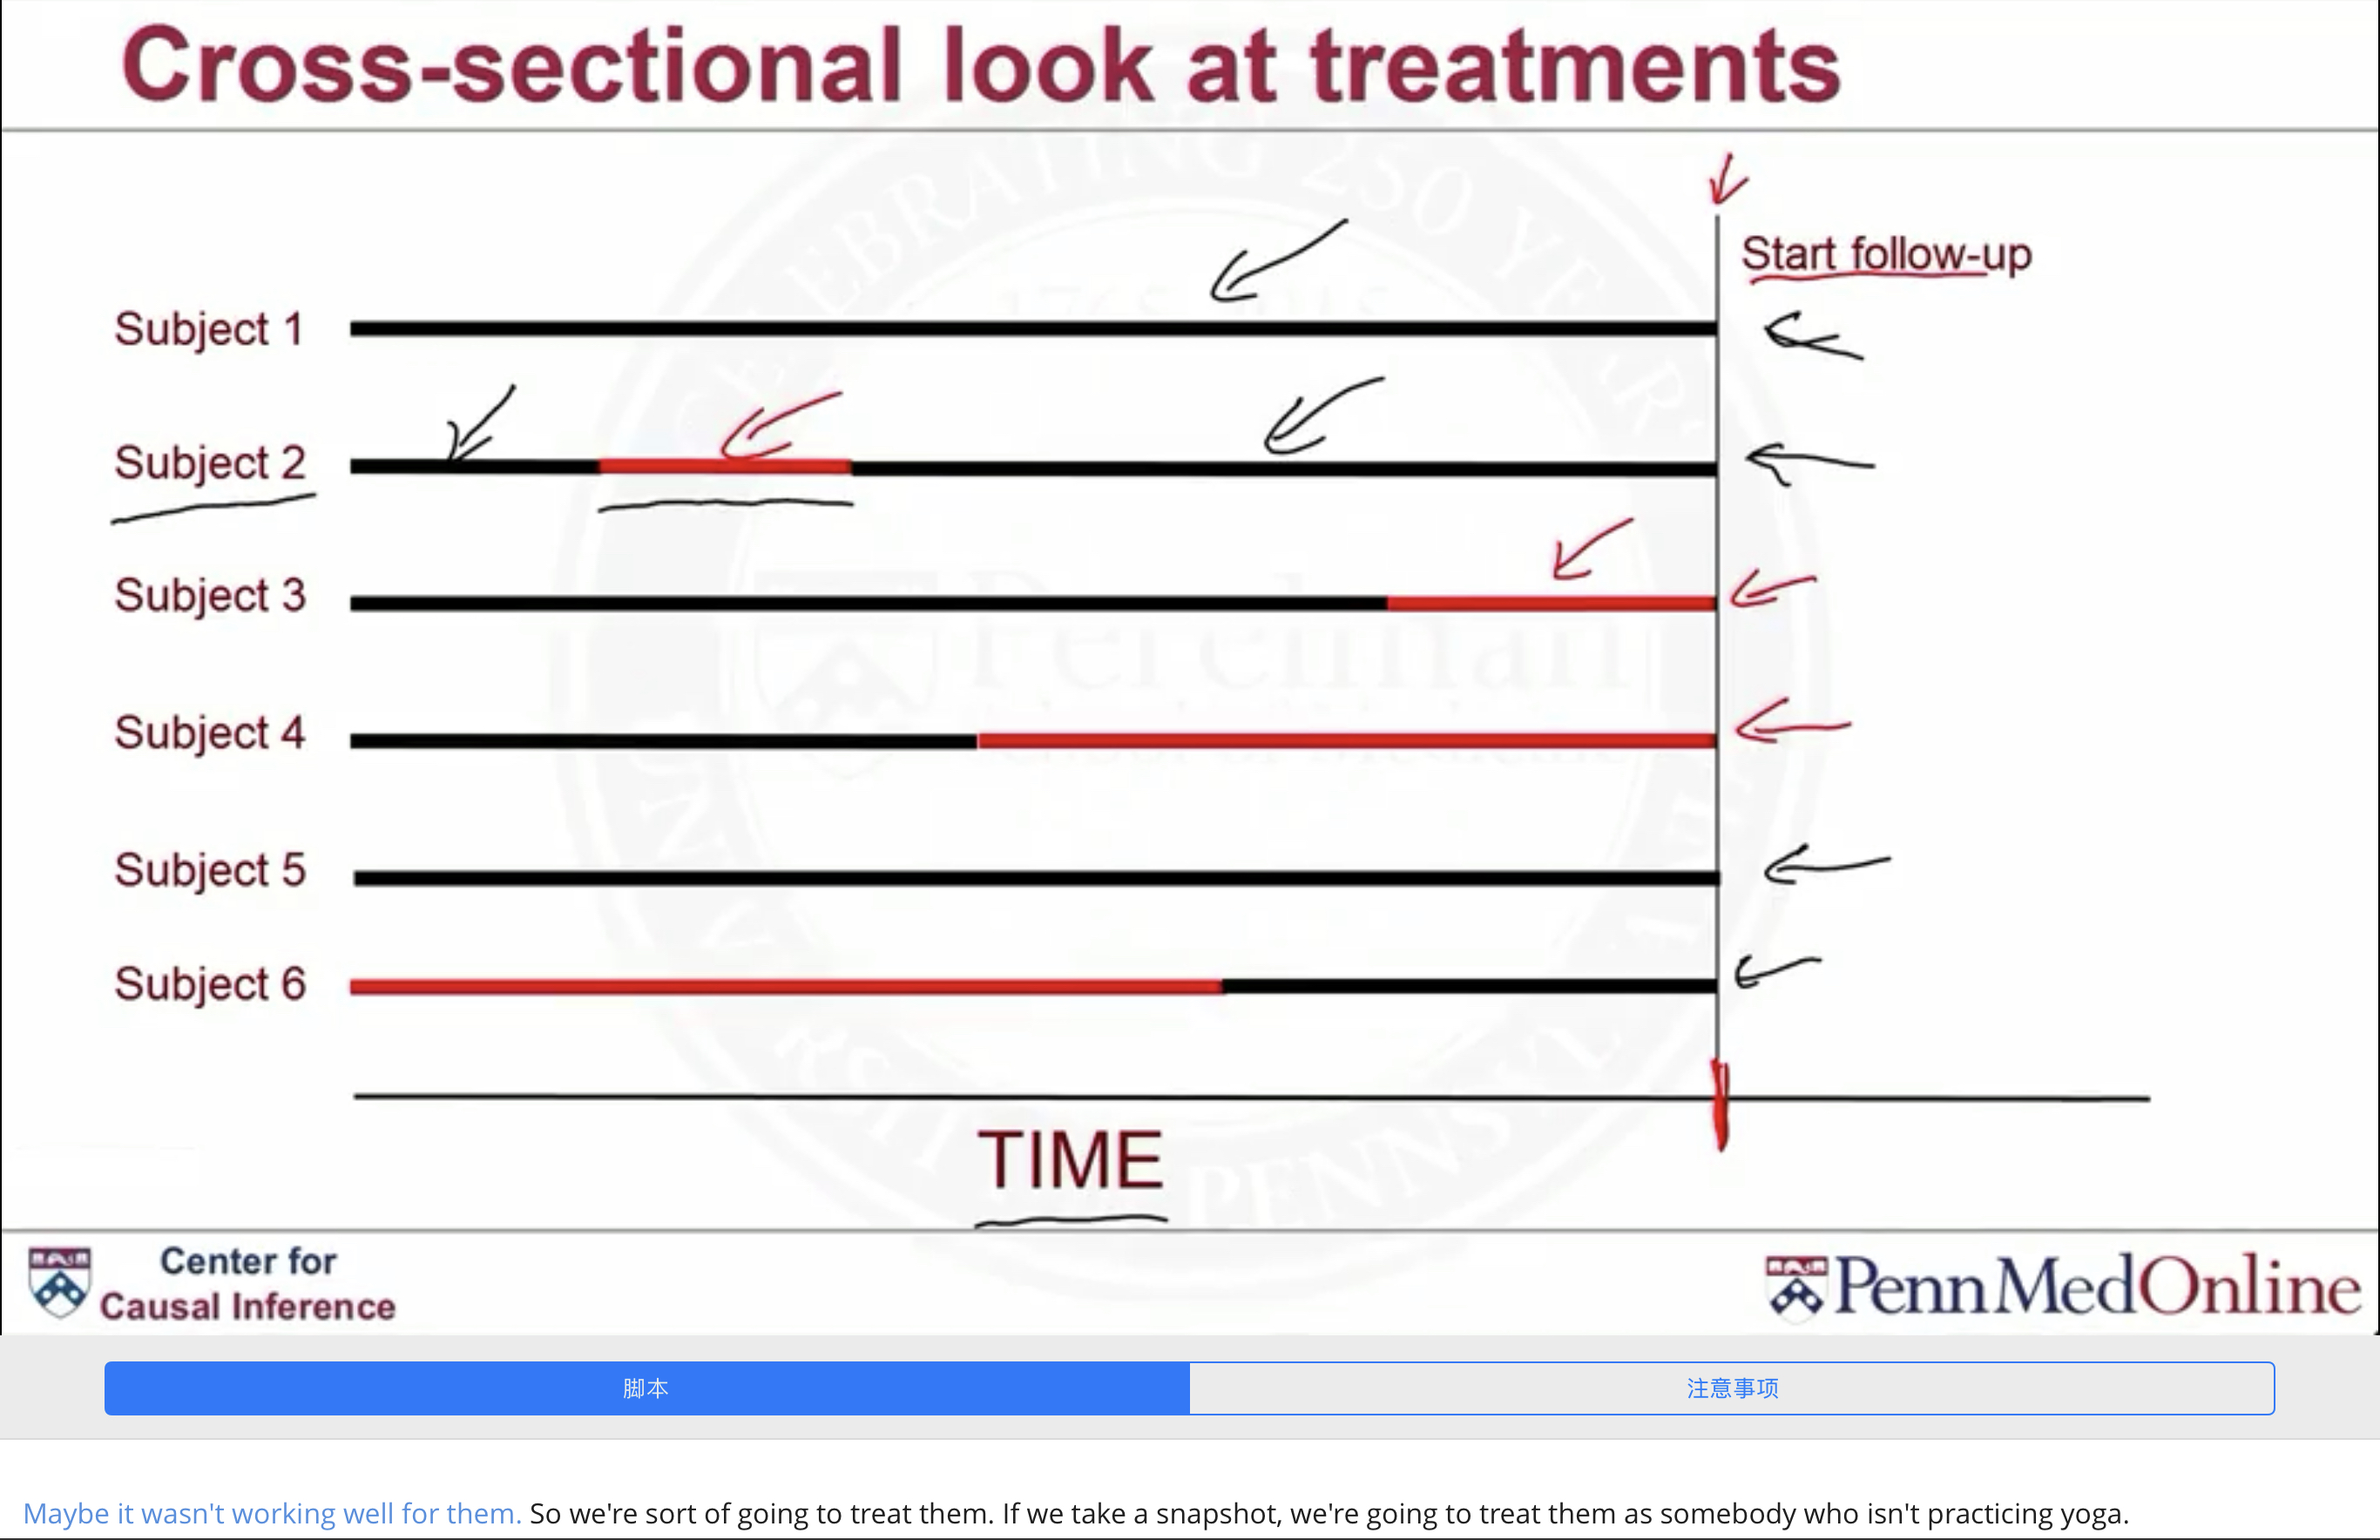
\includegraphics[width=0.8\textwidth]{figure/cstrt.jpg} 
	\caption{cross-sectional look at treatment}
	\label{cstrt}
\end{figure} 
Cross-sectional look 的问题在于:在观测节点之前,practicing yoga就已经产生了treatment effect,而这部分treatment effect又残留在新的观测数据中.

\subsection{New User design}
为解决上述问题,我们转而关注"people who newly initiaing treatment". 这种方法就是{\color{red} new user design}. 在new user design中,我们找到一些subjects刚好一致地从观测点开始treatment.

在这个过程中,关注的people发生了变换:
The treated people who is currently treated regardless of their treated history $\Longrightarrow$ new initiators. 

因此在某些程度上,我们关注的问题也发生了变化:
The causal effect of "practicing yoga" on "blood pressure" $\Longrightarrow$ the causal effect of "initiating practicing yoga" on "blood pressure". 

通过将问题转化成new user design,我们研究的causal effect就更加清楚,排除了上述的"selection bias"问题.
An example of new user design is given in Fig.\ref{nwud}:
\begin{figure}[htbp]
	\setlength{\abovecaptionskip}{0pt}     %调整图片标题与图距离
	\vspace{-0cm}  %调整图片与上文的垂直距离
	\setlength{\abovecaptionskip}{-0cm}   %调整图片标题与图距离
	\setlength{\belowcaptionskip}{0pt}   %调整图片标题与下文距离
	\centering
	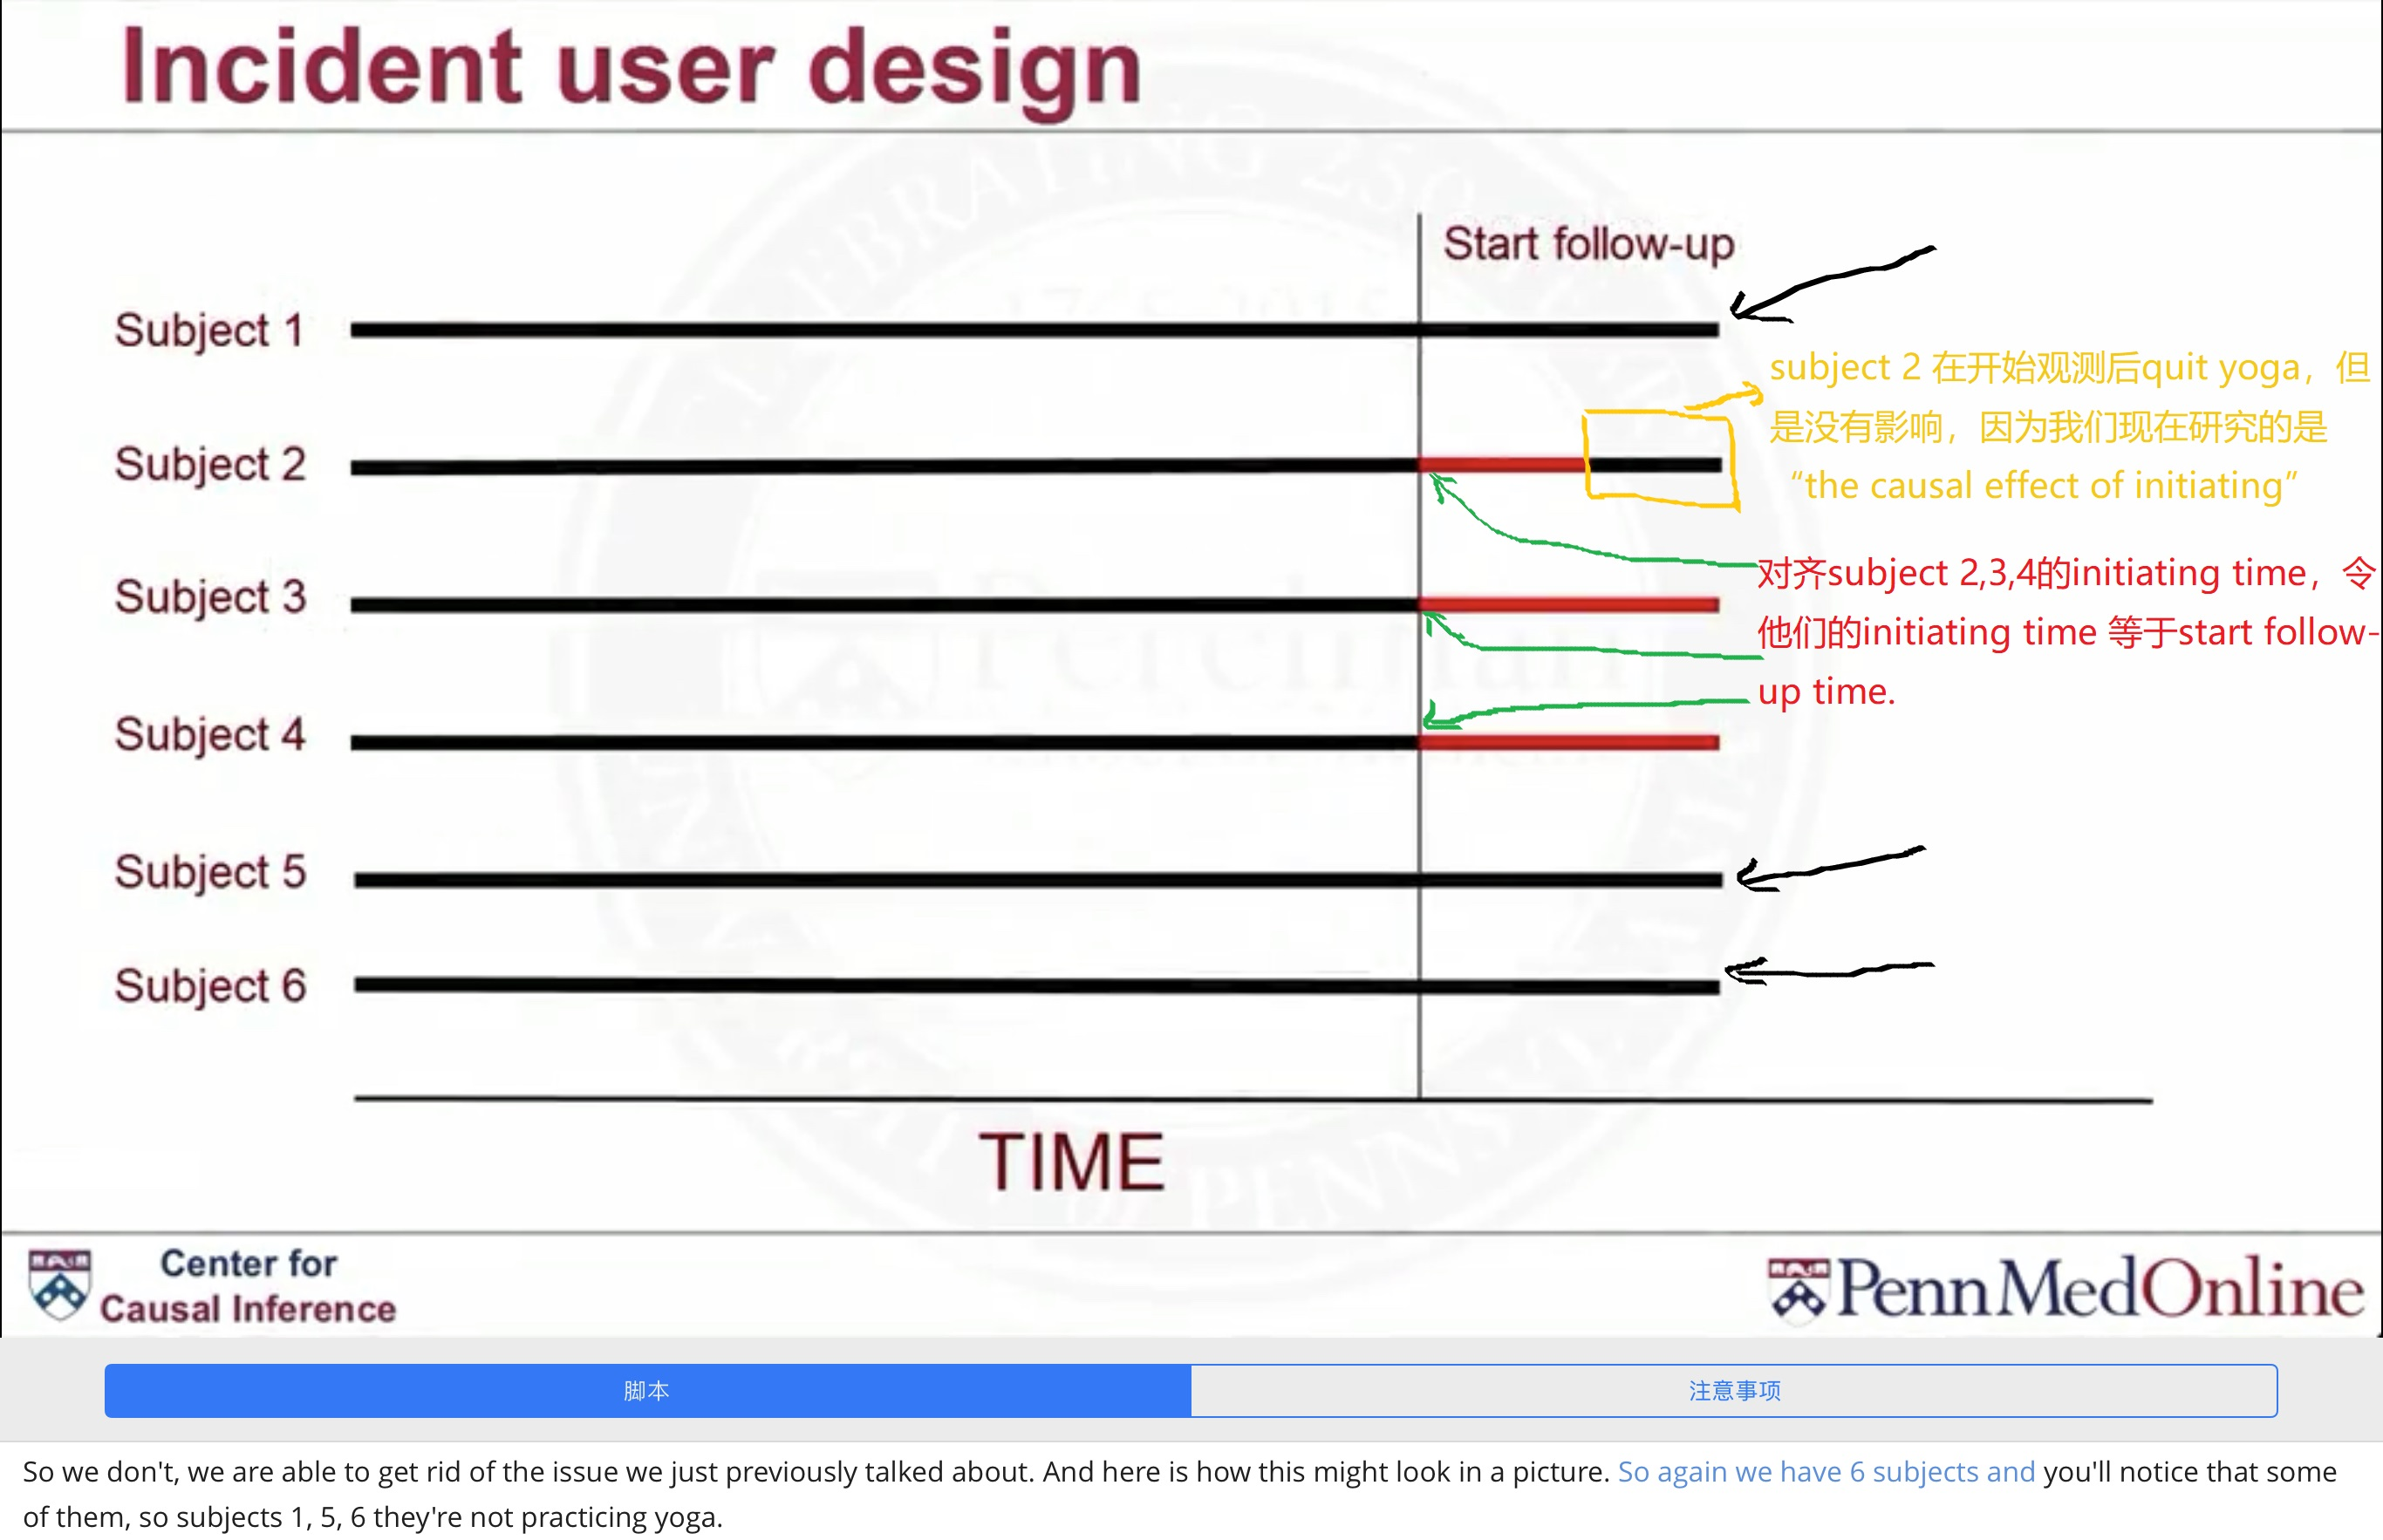
\includegraphics[width=0.8\textwidth]{figure/newud.jpg} 
	\caption{New user design}
	\label{newud}
\end{figure} 

\paragraph{The shortcome of incident user design:} 
\begin{enumerate}[label=\arabic*.]
	\item 我们已经注意到,incident user design将treated group限制在了{\color{red}"newly initiating treatment"的人群中,}因此我们只能考察{\color{red} “对于过去没有练过瑜伽的人,开始练习瑜伽后对血压的causal effect.”}
	\item {\bfseries It's hard to implement incident user design.} There's not going to be any period of time where people have no treatment.
    \item {\bfseries Untreated group的start follow-up问题.} 在New user design中,treated group中的subjects都有了明确的initiating time,我们可以设置start follow-up time,但是对于那些“从来没有接受过treatment”的人来说,start follow-up time却并不明确.
    \item {\bfseries Abvious difference between confounders of both groups.} 练习yoga的人和从不练习yoga的人在confounders上有着很大的不同,此时控制Confounders也是一个很大的问题.
\end{enumerate}

解决后面两个问题的一个方法是:再找一个treatment,与现有的treatment形成对比组. 这就是接下来要说的另一种design——active comparator design.

\subsection{Active Comparator Design}
如果比较两种treatment"initiate yoga"和"initiate Zumba"对于"blood pressure"的影响,问题就变成了"active comparator design".
Fig.\ref{acd}给出了两个具体的例子.
\begin{figure}[htbp]
	\setlength{\abovecaptionskip}{0pt}     %调整图片标题与图距离
	\setlength{\belowcaptionskip}{10pt}
	\vspace{-0cm}  %调整图片与上文的垂直距离
	\setlength{\abovecaptionskip}{-0cm}   %调整图片标题与图距离
	\setlength{\belowcaptionskip}{-0cm}   %调整图片标题与下文距离
	\centering
	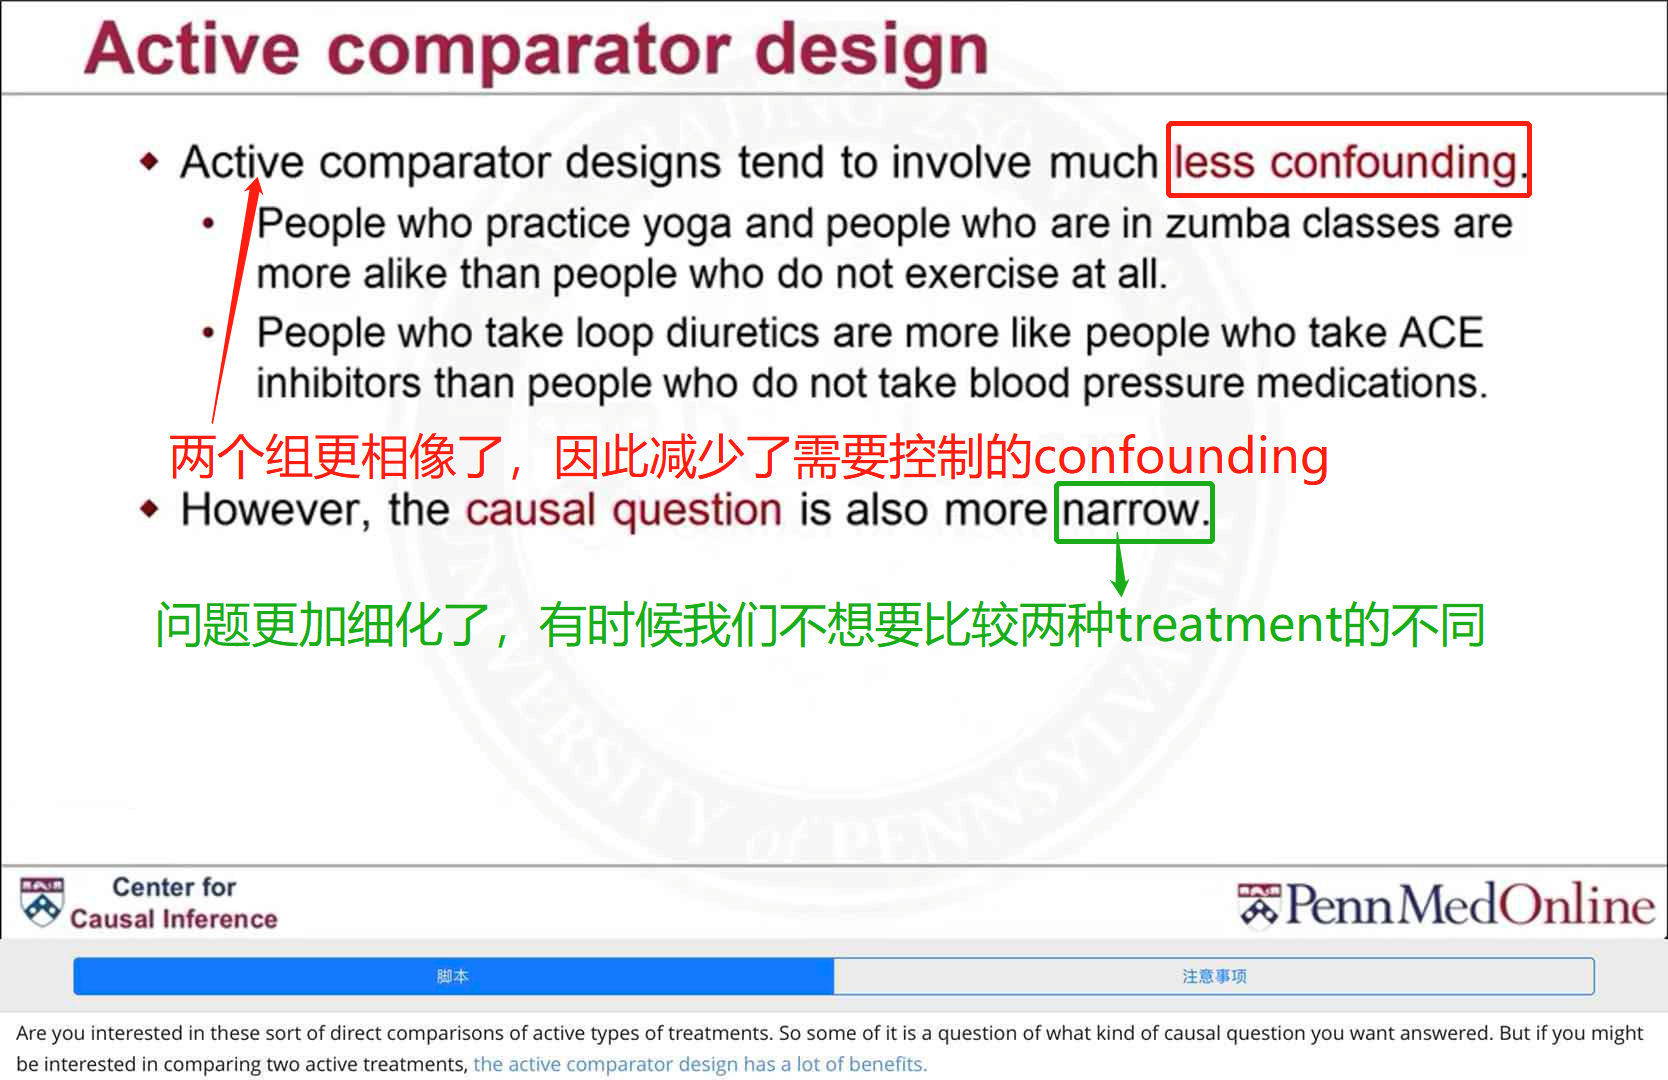
\includegraphics[width=0.8\textwidth]{figure/acd.png} 
	\caption{Active comparator design}
	\label{acd}
\end{figure} 

假设我们收集到了6个样本,如Fig.\ref{exacd}所示.
\begin{figure}[htbp]
	\setlength{\abovecaptionskip}{0pt}     %调整图片标题与图距离
	\setlength{\belowcaptionskip}{10pt}
	\vspace{-0cm}  %调整图片与上文的垂直距离
	\setlength{\abovecaptionskip}{-0cm}   %调整图片标题与图距离
	\setlength{\belowcaptionskip}{-0cm}   %调整图片标题与下文距离
	\centering
	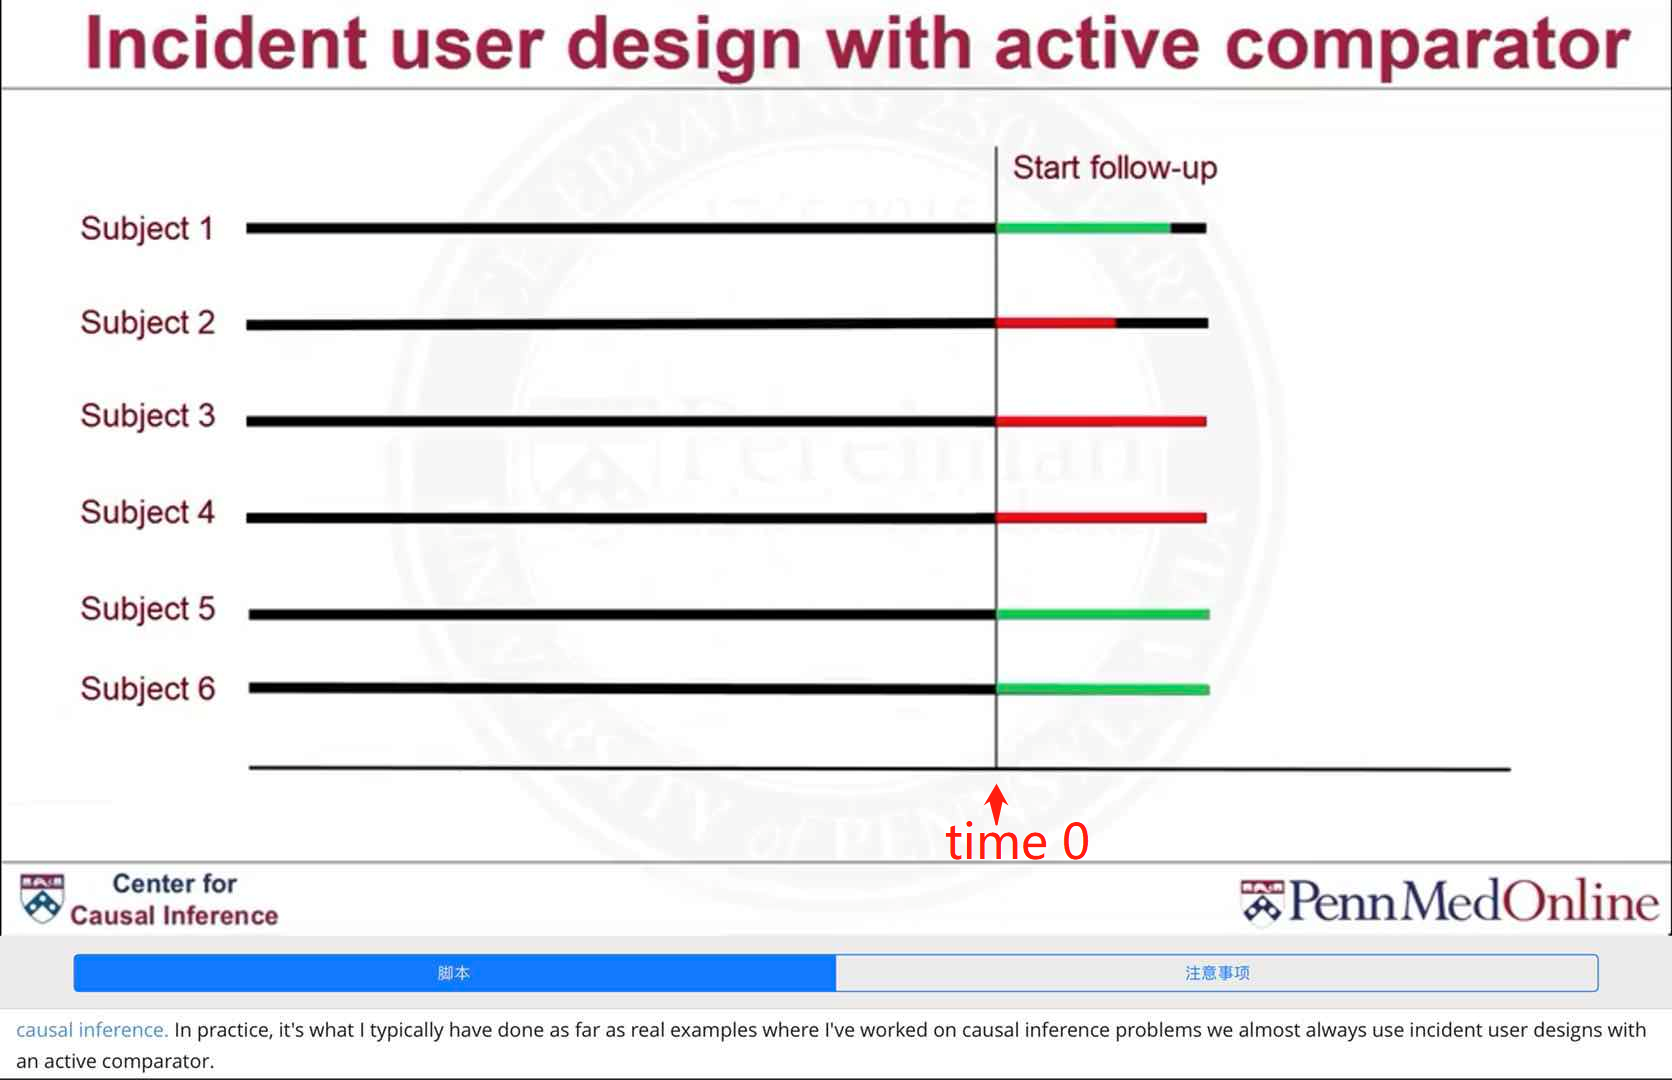
\includegraphics[width=0.8\textwidth]{figure/exacd.png} 
	\caption{New user design with active comparator}
	\label{exacd}
\end{figure} 

We note that the confounders that we can control for would be variables that were measured prior to time 0.

\paragraph{Issues of active comparator design.} 
\begin{enumerate}[label=\arabic*.]
	\item We are not interested in comparing to some active treatment. The causal question is too narrow.
	\item 与new user design的问题相同. There's not going to be any period of time where people have no treatment.
\end{enumerate}

\subsection{Conclusion}
最后总结一下这两种design存在的问题:
\begin{figure}[htbp]
	\setlength{\abovecaptionskip}{0pt}     %调整图片标题与图距离
	\setlength{\belowcaptionskip}{10pt}
	\vspace{-0cm}  %调整图片与上文的垂直距离
	\setlength{\abovecaptionskip}{-0cm}   %调整图片标题与图距离
	\setlength{\belowcaptionskip}{-0cm}   %调整图片标题与下文距离
	\centering
	
\includegraphics[width=0.8\textwidth]{figure/othercon.jpg} 
	\caption{Conclusion of the two designs}
	\label{othercon}
\end{figure} 

需要说明的是{\color{red}there are causal methods that can handle time variant treatments where we might be looking at the causal effects of treatments over time.}




    \chapter{Confounding and DAGs}
\section{Confounding}
\subsection{Ignorability and Confounding}
If the ignorability assumption is violated, treatment assignment depends on the potential outcomes. 可以举两个例子.

\begin{ex}
	研究某种药物的治疗效果,$A$表示是否接受治疗,$Y$表示康复人数,$X$表示病情. 病情严重的病人更有可能接受治疗,而病情轻微的病人更可能不采取治疗,因此在treated group,很多都是病情严重的病人,在control group大多数都是病情轻微的病人. 此时治疗的分配并不是随机的,treated group可能因为病情严重没有康复者,control group因为病情轻微可以自愈. 此时的outcome就与治疗的分配有关.
\end{ex}
\begin{ex}
	研究广告投放对未来用户登录量的影响. $A$表示是否被投放广告,$Y$表示未来5日登录人数,$X$表示过去1个月登录次数. 互联网公司更可能会对$X$小的用户投放广告,此时treated group中过去登录次数少的用户占了一大部分,即使对他们投放了广告,他们的$Y$也可能很小. 而control group原本就登录频繁,未来的$Y$也会比较大. 此时的outcome与广告的投放有关.
\end{ex}

从上面的例子我们看到,在treatment assignment与$X$有关时,如果不控制$X$,就违背了ignorability assumption,此时不能识别真实的causal effect.

\subsection{Confounding}
{\color{red} Confounders} are variables that affect both treatment and outcome. 

We note that the effect of $X$ to $Y$ is independent to the treatment. Fig.\ref{cslgph} shows the relationship between confounders, treatment and outcome.

\begin{figure}[htbp]
	\setlength{\abovecaptionskip}{0pt}     %调整图片标题与图距离
	\setlength{\belowcaptionskip}{10pt}
	\vspace{-0cm}  %调整图片与上文的垂直距离
	\setlength{\abovecaptionskip}{-0cm}   %调整图片标题与图距离
	\setlength{\belowcaptionskip}{-0cm}   %调整图片标题与下文距离
	\centering
	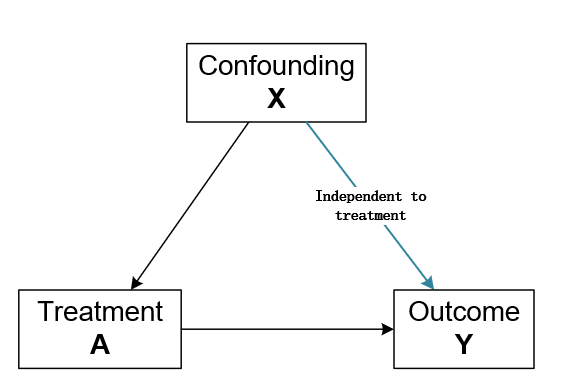
\includegraphics[width=0.4\textwidth]{figure/cslgph.png}
	\caption{Causal graph}
	\label{cslgph}
\end{figure}
	
如果一个变量并不是既影响treatmet又影响outcome,那么这个变量就不是confounder. Fig.\ref{exconfounder}所示.
\begin{figure}[htbp]
	\setlength{\abovecaptionskip}{0pt}     %调整图片标题与图距离
	\setlength{\belowcaptionskip}{10pt}
	\vspace{-0cm}  %调整图片与上文的垂直距离
	\setlength{\abovecaptionskip}{-0cm}   %调整图片标题与图距离
	\setlength{\belowcaptionskip}{-0cm}   %调整图片标题与下文距离
	\centering
	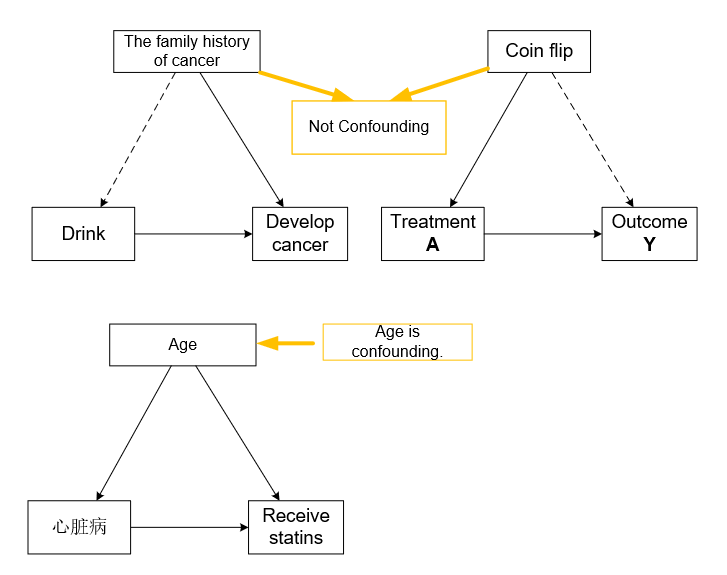
\includegraphics[width=0.8\textwidth]{figure/exconfounder.png}
	\caption{Distinguish confounders}
	\label{exconfounder}
\end{figure}

\subsection{Confounding Control}
\begin{enumerate}[label=(\arabic*)]
	\item {\bfseries 重要性}:Identifying a set of variables $X$, 以保证ignorability assumption成立. {\hl The set of variables is sufficient to control for confounding.}
	\item 用什么方法control this set of variables?
\end{enumerate}

\section{Causal Graph} \label{Causalgraph}
Causal graph: directed acyclic graph.
\subsection{The importance of causal graph}
1. Make assumptions explicit:DAG depicts the assumptions we making on the relationship between variables.

2.Helpful for identifying which variables to control for.

\subsection{Simple graph}
Directed graph $A \longrightarrow Y$: $A$ affects $Y$.

Undirected graph A $\rule[4pt]{0.8cm}{0.05em}$ Y: $A$ is associated with $Y$.\\

\subsection{Graphical models}
\begin{itemize}
	\item 图模型反映了变量之间的independence、dependence、conditional independence的关系. 我们能做的是通过observed data去验证因果图显示的关系是否存在.
	\item 推导非参数的因果效应估计量.(后面会讲到.)
\end{itemize}

\subsection{Terminology}
这一部分讲到了DAG的专业名词:node(vertice), link(edge), path, parent, child, ancestor, descendant.

\paragraph{Path:}与原来认识的path不同. 这里的path并不局限于指向同一方向的路径,指向同一方向的path称为chain,我们后面会讲到另外两种path,称为fork和inverted fork.
\begin{ex}
	在Fig.\ref{expath}中,我们可以找到4条从D到B的path,分别是:\\
	(1) D $\longrightarrow$ A $\longrightarrow$ B; \\
	(2) D $\longrightarrow$ A $\longleftarrow$ G $\longrightarrow$ B;\\
	(3) D $\longrightarrow$ E $\longrightarrow$ G $\longrightarrow$ B;\\
	(4) D $\longrightarrow$ E $\longrightarrow$ G
	$\longrightarrow$ A $\longrightarrow$ B;
\end{ex}
\begin{figure}[htbp]
	\setlength{\abovecaptionskip}{0pt}     %调整图片标题与图距离
	\setlength{\belowcaptionskip}{10pt}
	\vspace{-0cm}  %调整图片与上文的垂直距离
	\setlength{\abovecaptionskip}{-0cm}   %调整图片标题与图距离
	\setlength{\belowcaptionskip}{-0cm}   %调整图片标题与下文距离
	\centering
	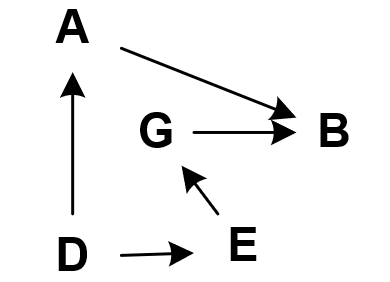
\includegraphics[width=0.2\textwidth]{figure/expath.png}
	\caption{Example of paths}
	\label{expath}
\end{figure}

\paragraph{Parents and ancestors} we look at a chain in Fig.\ref{expath}: 
\begin{equation}
D \longrightarrow E \longrightarrow G.
\end{equation}
	
	In this chain, E is the child of D, and D is the parent of E. D and E are the ancestors of G, and E and G are the descendants of D.


\subsection{DAGs}
DAGs的条件:
\begin{itemize}
	\item 不存在undirected edge.
	\item No circle.
\end{itemize}

\subsection{conclusion}
最后总结一下这一课的重点:
\begin{figure}[htbp]
	\setlength{\abovecaptionskip}{0pt}     %调整图片标题与图距离
	\setlength{\belowcaptionskip}{10pt}
	\vspace{-0cm}  %调整图片与上文的垂直距离
	\setlength{\abovecaptionskip}{-0cm}   %调整图片标题与图距离
	\setlength{\belowcaptionskip}{-0cm}   %调整图片标题与下文距离
	\centering
	
\includegraphics[width=0.8\textwidth]{figure/dagconclusion.jpg}
	\caption{Conclusion of DAGs}
	\label{dagconclusion}
\end{figure}


\newpage \section{Relationship between DAGs and probability distributions}
\noindent {\bfseries Outline:}\\
1. The relationship between DAGs and probability distributions.\\
2. Decomposition of joint distribution.\\
3. Compatibility of DAGs and probability.
\subsection{The relationship between DAGs and probability distributions} 
在\ref{Causalgraph}中,我们说到DAG可以反映出variables之间的independence, dependence, conditional independence关系. 对于DAG中的所有nodes,DAG编码了它们之间joint distribution的假设. 下面举例说明DAG能向我们传达什么信息.
\begin{ex}
	从Fig.\ref{DAGex1}的因果图中,我们可以解码出4个节点的联合分布信息:
    \begin{itemize}
    	\item P(C$|$A,B,D) = P(C), i.e., C与A,B,D独立. Conditional on A,B,D, does not tell any information about the probability of C.
        {\b \item P(A$|$B,C,D) = P(A$|$B,D) }
    	\item P(B$|$A,C,D) = P(B$|$A,D)=p(B$|$A), i.e., B$\perp$D$|$A. D对B的影响都是通过A作用的,当给定A时,D对A的作用也包含在A里面了,此时D不再给B的分布提供额外的信息.
    	\item P(B$|$D) $\neq$ P(B), B and D are (marginally) dependent. 在上一则item中我们知道给定A时,B和D是条件独立的. 然而尽管D对B的作用不是直接的,但是D与B却是边缘相关的. {\color{orange} 可以这样理解:把D的作用从B中控制住,剩余部分的分布很明显不能等于原始B的分布.}	
    	\item P(D$|$A,B,C) = P(D$|$A,B) = P(D$|$A), B与D的相关是通过A的,给定A之后,B就不能对D的分布提供额外信息了.
    \end{itemize}
\end{ex}
	\begin{figure}[htbp]
	\setlength{\abovecaptionskip}{0pt}     %调整图片标题与图距离
	\setlength{\belowcaptionskip}{10pt}
	\vspace{-0cm}  %调整图片与上文的垂直距离
	\setlength{\abovecaptionskip}{-0cm}   %调整图片标题与图距离
	\setlength{\belowcaptionskip}{-0cm}   %调整图片标题与下文距离
	\centering
	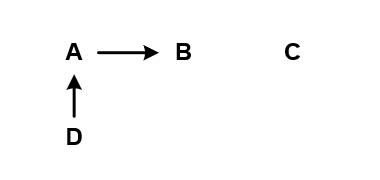
\includegraphics[width=0.4\textwidth]{figure/DAGex1.png}
	\caption{Example 1}
	\label{DAGex1}
    \end{figure}

\begin{ex}
	从Fig.\ref{DAGex2}的因果图中,我们可以解码出4个节点的联合分布信息:
	\begin{itemize}
		\item P(A$|$B,C,D) = P(A$|$D), 对A产生影响的只有D,给定D,我们就知道了关于A的所有.
		\item P(D$|$A,B,C) = P(D$|$A,B), {\color{red} D对A,B分别有独立的影响,所以A,B之中独立地蕴含了与D有关的信息.} {\color{orange} 虽然C与D也有关系,但是是通过B作用的,给定B之后,C中就不包含对D有用的信息了.}
	\end{itemize}
\end{ex}

	
	\begin{figure}[htbp]
	\setlength{\abovecaptionskip}{0pt}     %调整图片标题与图距离
	\setlength{\belowcaptionskip}{10pt}
	\vspace{-0cm}  %调整图片与上文的垂直距离
	\setlength{\abovecaptionskip}{-0cm}   %调整图片标题与图距离
	\setlength{\belowcaptionskip}{-0cm}   %调整图片标题与下文距离
	\centering
	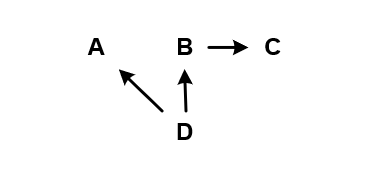
\includegraphics[width=0.4\textwidth]{figure/DAGex2.png}
	\caption{Example 2}
	\label{DAGex2}
    \end{figure}


\begin{ex}
	从Fig.\ref{DAGex3}的因果图中,我们可以解码出4个节点的联合分布信息:
    \begin{itemize}
    	\item P(A$|$B,C,D) = P(A$|$C,D),从path的角度来讲, B到A没有path, 可以直接把B去掉.
    	\item P(D$|$A,B,C) = P(D$|$A,B), 从path的角度来讲,C对D的影响都是通过A和B的,给了A和B之后,C中就不包含对D的分布有用的信息了.
    \end{itemize}
\end{ex}

	\begin{figure}[htbp]
	\setlength{\abovecaptionskip}{0pt}     %调整图片标题与图距离
	\setlength{\belowcaptionskip}{10pt}
	\vspace{-0cm}  %调整图片与上文的垂直距离
	\setlength{\abovecaptionskip}{-0cm}   %调整图片标题与图距离
	\setlength{\belowcaptionskip}{-0cm}   %调整图片标题与下文距离
	\centering
	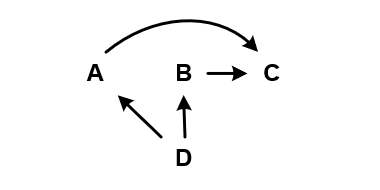
\includegraphics[width=0.4\textwidth]{figure/DAGex3.png}
	\caption{Example 3}
	\label{DAGex3}
\end{figure}

\subsection{Decomposition fo Joint Distribution}
在上面的3个例子,将节点的联合分布分解: 
\begin{enumerate}[label=(\arabic*)]
	\item P(A,B,C,D) = P(B$|$A)P(A$|$D)P(D)P(C)
	\item P(A,B,C,D) = P(C$|$B)P(B$|$D)P(A$|$D)P(D)
    \item P(A,B,C,D) = P(C$|$A,B)P(A$|$D)P(B$|$D)P(D)
\end{enumerate}

\subsection{Compatibility}
这一部分探讨的是DAG与Probability function能不能{\bfseries 互推}. 举个例子.
\begin{ex}
Probability distribution: P(A,B) $ \neq$ P(A)P(B). There are 2 DAGs compatible with this probability:
A $\longrightarrow$ B, and A $\longleftarrow $B.
\end{ex}

说明{\color{red}一个probability function对应的DAG并不是唯一的}.
因此我们使用DAG来表示变量关系,而不是probability function.


\newpage\section{Paths and associations}
\subsection{Types of Paths}
(1) Fork: information flows from one node to different nodes. Fig.\ref{fork} shows the basic structure of fork.
	\begin{figure}[htbp]
	\setlength{\abovecaptionskip}{0pt}     %调整图片标题与图距离
	\setlength{\belowcaptionskip}{10pt}
	\vspace{-0cm}  %调整图片与上文的垂直距离
	\setlength{\abovecaptionskip}{-0cm}   %调整图片标题与图距离
	\setlength{\belowcaptionskip}{-0cm}   %调整图片标题与下文距离
	\centering
	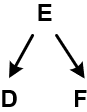
\includegraphics[width=0.1\textwidth]{figure/fork.png}
	\caption{Fork}
	\label{fork}
    \end{figure}

(2) Chain: information flows in one direction. Fig.\ref{chain} shows the basic structure of chain.
	\begin{figure}[htbp]
	\setlength{\abovecaptionskip}{0pt}     %调整图片标题与图距离
	\setlength{\belowcaptionskip}{10pt}
	\vspace{-0cm}  %调整图片与上文的垂直距离
	\setlength{\abovecaptionskip}{-0cm}   %调整图片标题与图距离
	\setlength{\belowcaptionskip}{-0cm}   %调整图片标题与下文距离
	\centering
	
\includegraphics[width=0.2\textwidth]{figure/chain.png}
	\caption{Chain}
	\label{chain}
    \end{figure}

(3)Inverted forks: Information flows from different nodes to one node. 
	\begin{figure}[htbp]
	\setlength{\abovecaptionskip}{0pt}     %调整图片标题与图距离
	\setlength{\belowcaptionskip}{10pt}
	\vspace{-0cm}  %调整图片与上文的垂直距离
	\setlength{\abovecaptionskip}{-0cm}   %调整图片标题与图距离
	\setlength{\belowcaptionskip}{-0cm}   %调整图片标题与下文距离
	\centering
	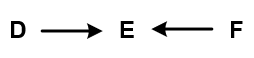
\includegraphics[width=0.2\textwidth]{figure/invfork.png}
	\caption{Inverted fork}
	\label{invfork}
    \end{figure}
In Fig.\ref{invfork}, "E" is called as "Collider". It's the junction of information.

\subsection{Relationship between varaibles in 3 types of paths}
(1) {\bfseries Induce dependence of E and F:} Fork and chain. 
\begin{itemize}
	\item In fork path, the information in E flows to both D and F, so D and F are dependent.  
	\item In chain path, the information in D flows to E and then flows to F. Or we can say that D affects E and then E affects F. So E and F are obviously dependent. {\g  {Most importantly, it is E that really causing this association between D and F.}}
\end{itemize}

(2) {\bfseries Induce independece of E and F:} Inverted fork. 
\begin{itemize}
	\item There is no information flows to E from F, and there is also no information flows to F from E. So E and F are independent.
\end{itemize}

\section{Conditional independence(d-separation)}
\subsection{Blocking}
Path can be blocked by conditioning on nodes in the path.

\subsection{Blocking on chain}
Consider the path: $A \longrightarrow G\longrightarrow B$. 

A and B are dependent, but they are dependent through G, A affects G and then G affects B. So it is G that really causing this association between A and B. 

If we condition on the node in the middle of the chain, i.e.,G, we block the path from A to B. {\r {Then A is independent with B.} }

\begin{ex}
Suppose in the given chain path above,  A is temperature. G is whether sidewalk icy or not. B is whether someone falls or not. 

Temperature affects whether the sidewalk is icy or not. And the sidewalk is icy or not affects if someone falls. So temperature is associated with whether someone falls.

Now if we condition on G, say, the sidewalk is icy, then whether someone falling down is not associated with temperature. 
\end{ex}
这告诉我们,控制一条chain path中间的nodes,可以阻断两端nodes的相关性(association).

\subsection{Blocking on fork}
Consider in the fork: $A \longleftarrow G \longrightarrow B$.
We condition on G, making G the same for everyone. Then there is no relationship between A, G and B, i.e., G is no longer affecting A and B because we're holding it fixed.

If we condition on G, the association between A and B is blocked. 

\subsection{Blocking on inverted fork}
{\color{red} The opposite situation occurs if a collider is conditioned on.}
Consider the inverted fork path: $A \longrightarrow G \longleftarrow B$.

A and B are independent in the path, but conditioning on G induces an association between A and B.

\begin{ex}
	Here we give an example as shown in Fig.\ref{blockcollider1} and Fig.\ref{blockcollider2}. 
		\begin{figure}[htbp]
		\setlength{\abovecaptionskip}{0pt}     %调整图片标题与图距离
		\setlength{\belowcaptionskip}{10pt}
		\vspace{-0cm}  %调整图片与上文的垂直距离
		\setlength{\abovecaptionskip}{-0cm}   %调整图片标题与图距离
		\setlength{\belowcaptionskip}{-0cm}   %调整图片标题与下文距离
		\centering
		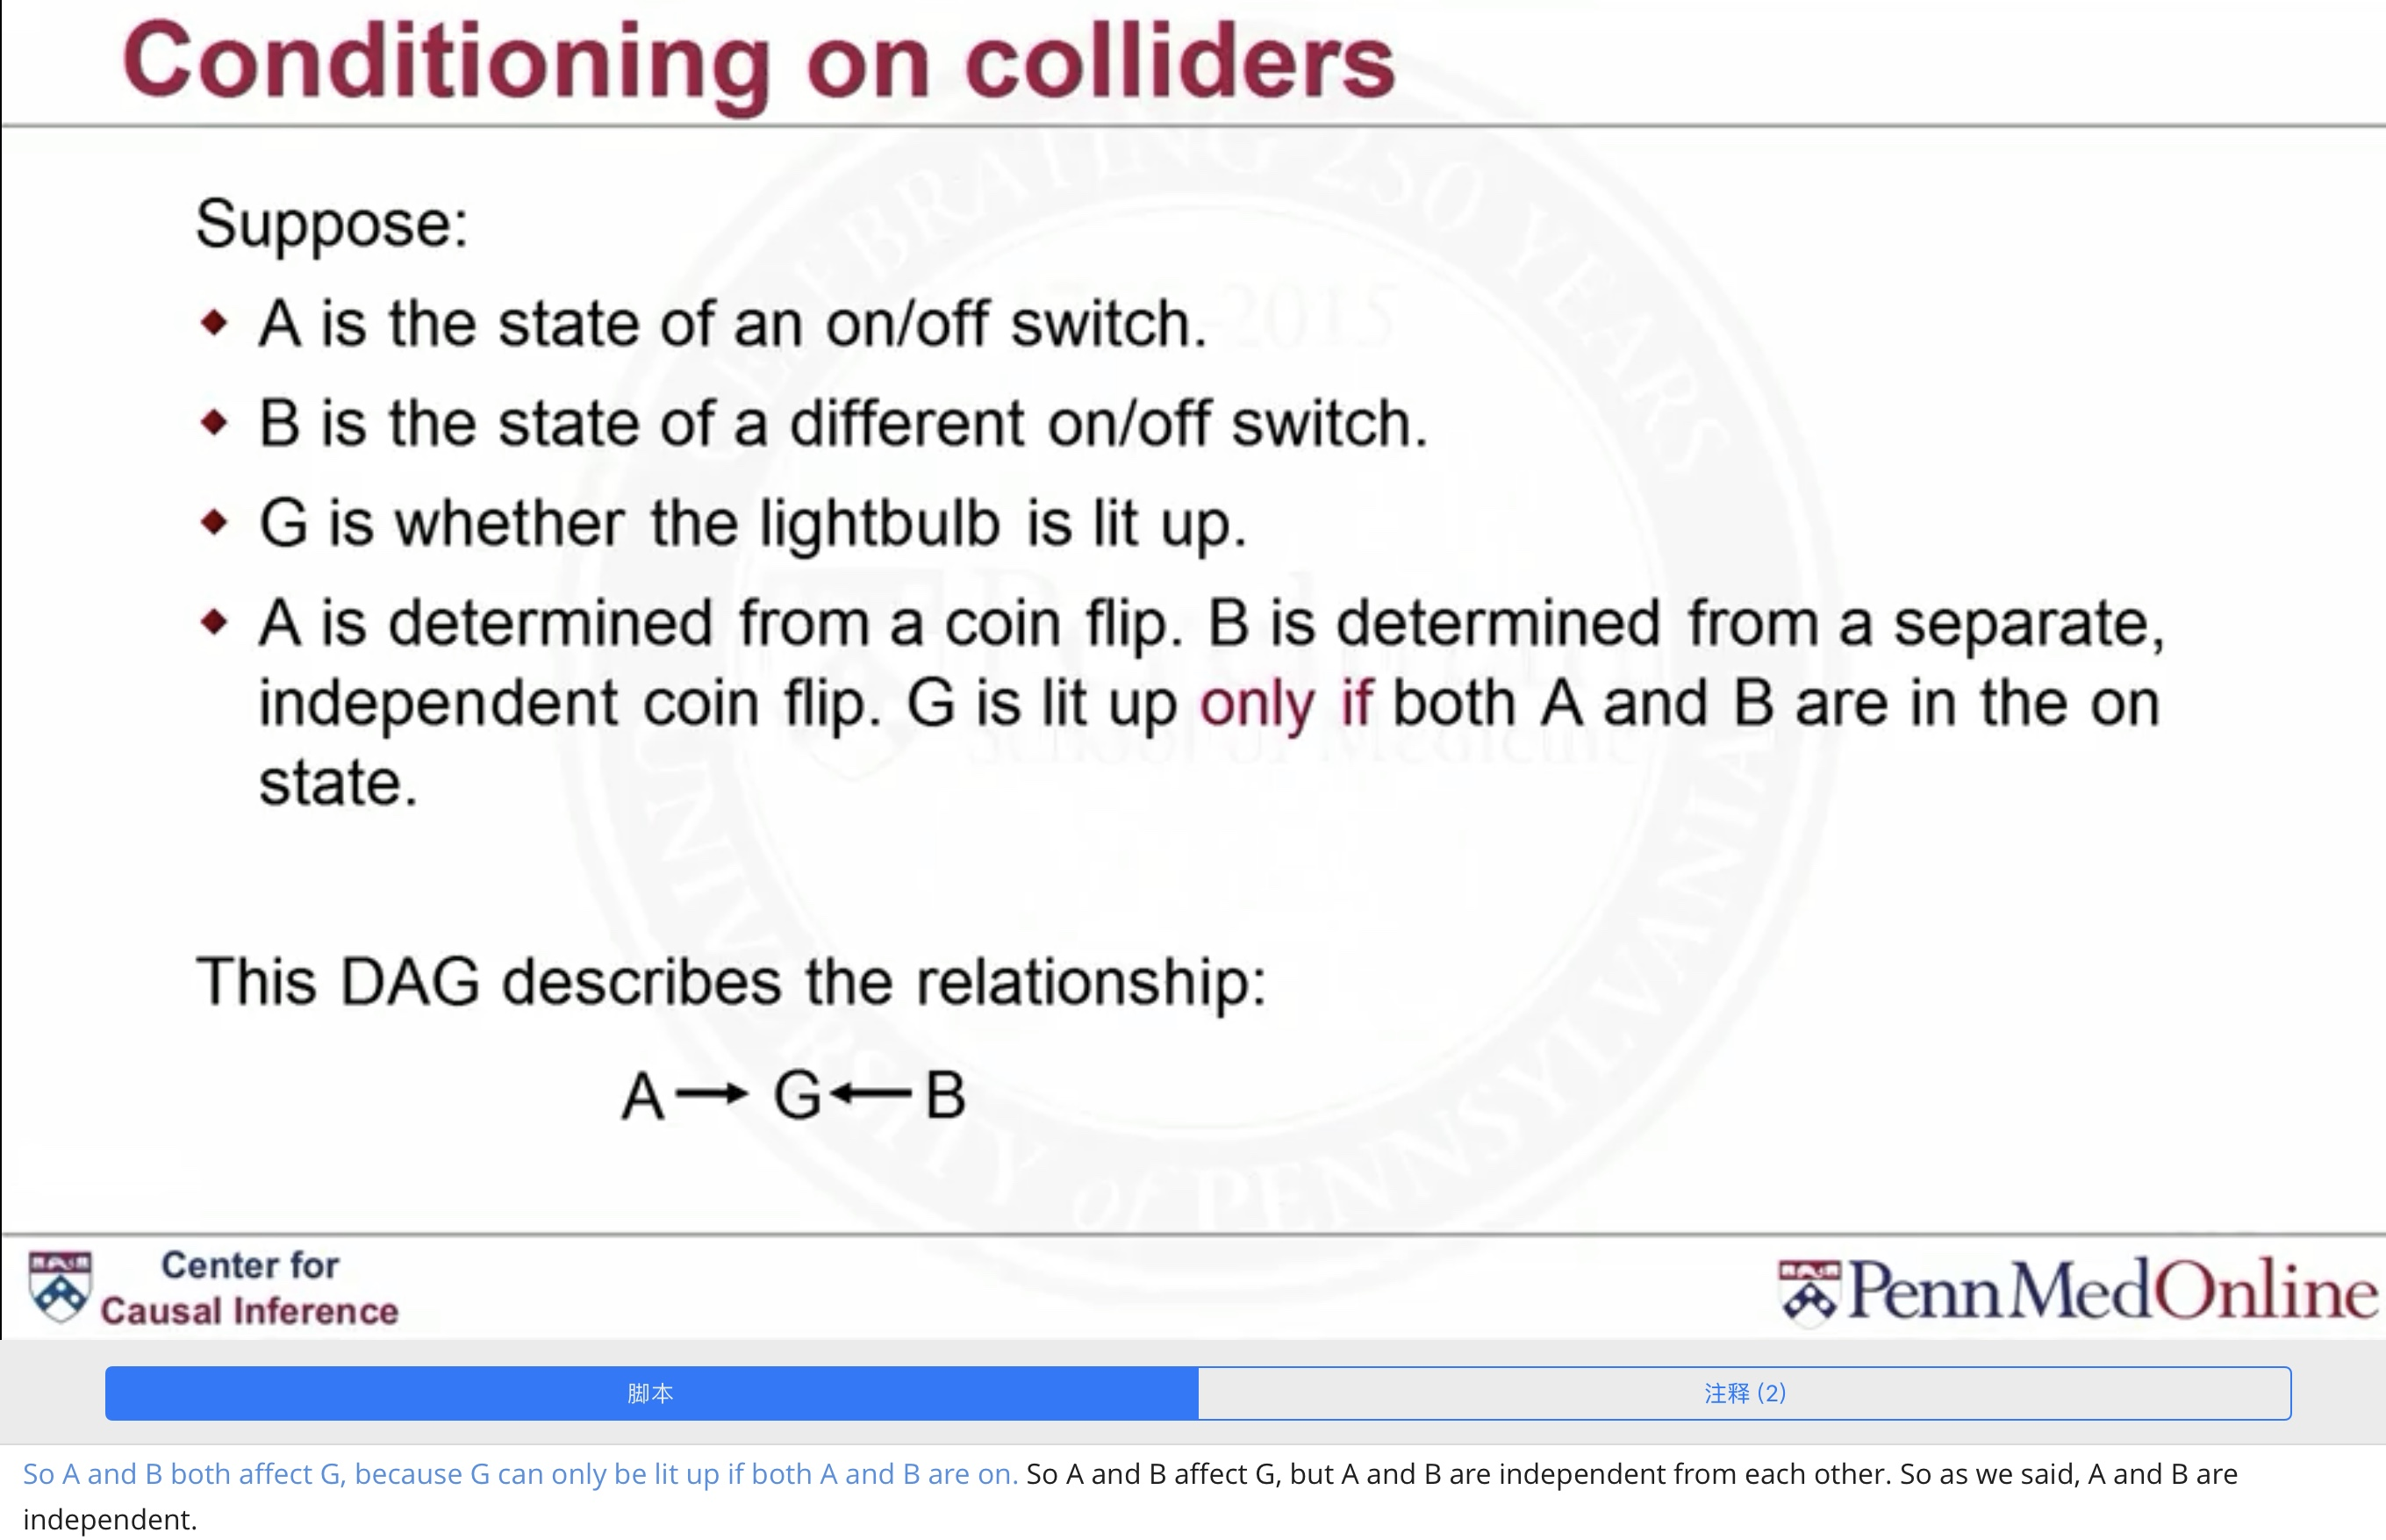
\includegraphics[width=0.8\textwidth]{figure/blockcollider1.jpg}
		\caption{Conditioning on collider(1)}
		\label{blockcollider1}
	\end{figure}

	\begin{figure}[htbp]
	\setlength{\abovecaptionskip}{0pt}     %调整图片标题与图距离
	\setlength{\belowcaptionskip}{10pt}
	\vspace{-0cm}  %调整图片与上文的垂直距离
	\setlength{\abovecaptionskip}{-0cm}   %调整图片标题与图距离
	\setlength{\belowcaptionskip}{-0cm}   %调整图片标题与下文距离
	\centering
	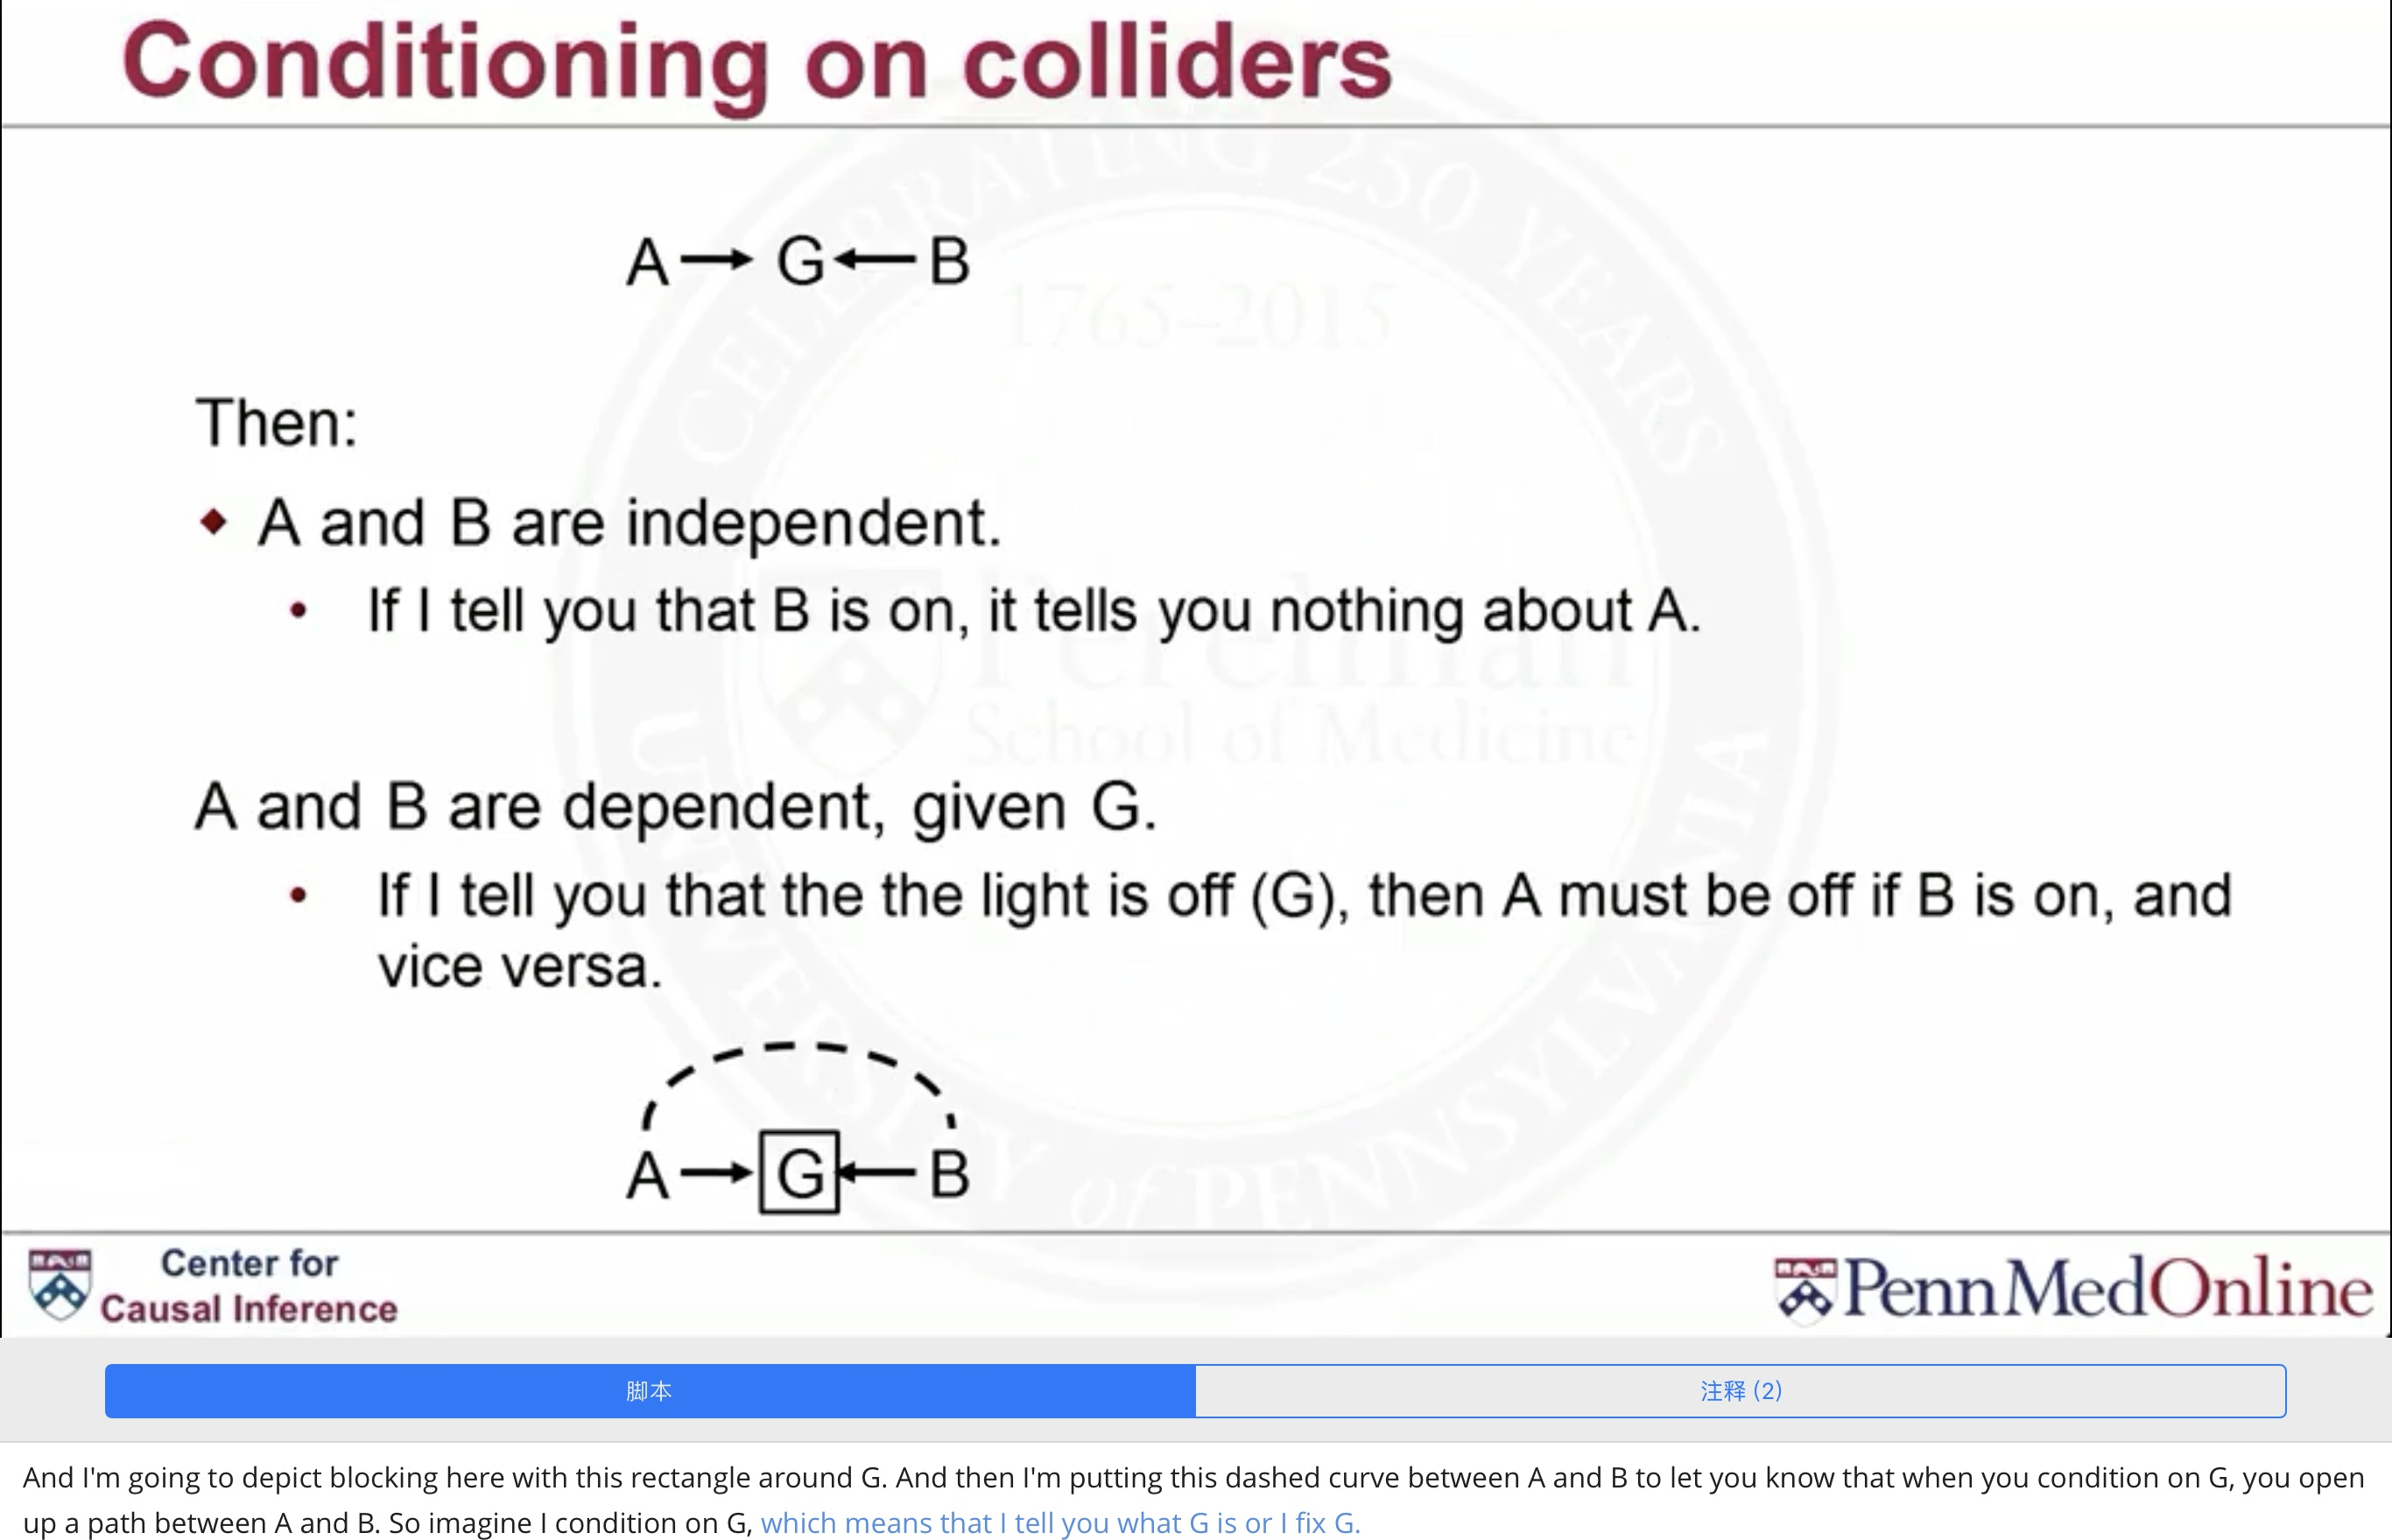
\includegraphics[width=0.8\textwidth]{figure/blockcollider2.jpg}
	\caption{Conditioning on collider(2)}
	\label{blockcollider2}
\end{figure}
	
\end{ex}

\subsection{Conclusion}
\begin{itemize}
	\item Controlling middle part of {\r {fork and chain}} will remove dependence. 
	\item Controlling collider of {\r {inverted fork}} will induce dependence. 
\end{itemize}



\section{Confounding revisited}
\noindent {\bfseries Outline:} \\
1. Frontdoor paths. \\
2. Backdoor paths. Why backdoor path needs to be blocked?

\subsection{Frontdoor path}
{\bfseries Frontdoor path is path that from treatment A to outcome Y. }There may be several nodes in the middle of the path from A to Y. A $\longrightarrow$ Z $\longrightarrow$ Y. As shown in Fig.\ref{frontdoor}.
	\begin{figure}[htbp]
	\setlength{\abovecaptionskip}{0pt}     %调整图片标题与图距离
	\setlength{\belowcaptionskip}{10pt}
	\vspace{-0cm}  %调整图片与上文的垂直距离
	\setlength{\abovecaptionskip}{-0cm}   %调整图片标题与图距离
	\setlength{\belowcaptionskip}{-0cm}   %调整图片标题与下文距离
	\centering
	
\includegraphics[width=0.8\textwidth]{figure/frontdoor.jpg}
	\caption{Frontdoor path}
	\label{frontdoor}
    \end{figure}
我们感兴趣的是A对Y的causal effect,而不在意A是通过什么作用到Y的. {\bfseries 就算A对Y的causal effect中有一部分是通过A对Z的causal effect实现的,也没有关系. } 我们并不关注这一部分,也就是说 {\color{red} 我们并不需要Control在frontdoor path上出现的variables.}

\subsection{Backdoor path}
{\bfseries Backdoor path is path that from treatment A to Y that travel through arrows {\color{orange}going into} A.}  As shown in Fig.\ref{backdoor}.
	\begin{figure}[htbp]
	\setlength{\abovecaptionskip}{0pt}     %调整图片标题与图距离
	\setlength{\belowcaptionskip}{10pt}
	\vspace{-0cm}  %调整图片与上文的垂直距离
	\setlength{\abovecaptionskip}{-0cm}   %调整图片标题与图距离
	\setlength{\belowcaptionskip}{-0cm}   %调整图片标题与下文距离
	\centering
	
\includegraphics[width=0.8\textwidth]{figure/backdoor.jpg}
	\caption{Backdoor path}
	\label{backdoor}
\end{figure}
如果我们只关注A与Y的边缘相关的话,其中一部分相关性是由于A对Y的causal effect造成的. 但是这部分causal effect中还有一部分是由于X对A的影响造成的. 

因此backdoor path影响了A对Y的真实causal effect的估计,我们需要backdoor path加以阻隔. 

如果我们block all backdoor paths,那么就可以满足ignorability assumption: $Y^0,Y^1 \perp A|X$. 也就是说我们需要寻找一个变量集X,这个变量集里的variables可以block all backdoor paths.
	\begin{figure}[htbp]
	\setlength{\abovecaptionskip}{0pt}     %调整图片标题与图距离
	\setlength{\belowcaptionskip}{10pt}
	\vspace{-0cm}  %调整图片与上文的垂直距离
	\setlength{\abovecaptionskip}{-0cm}   %调整图片标题与图距离
	\setlength{\belowcaptionskip}{-0cm}   %调整图片标题与下文距离
	\centering
	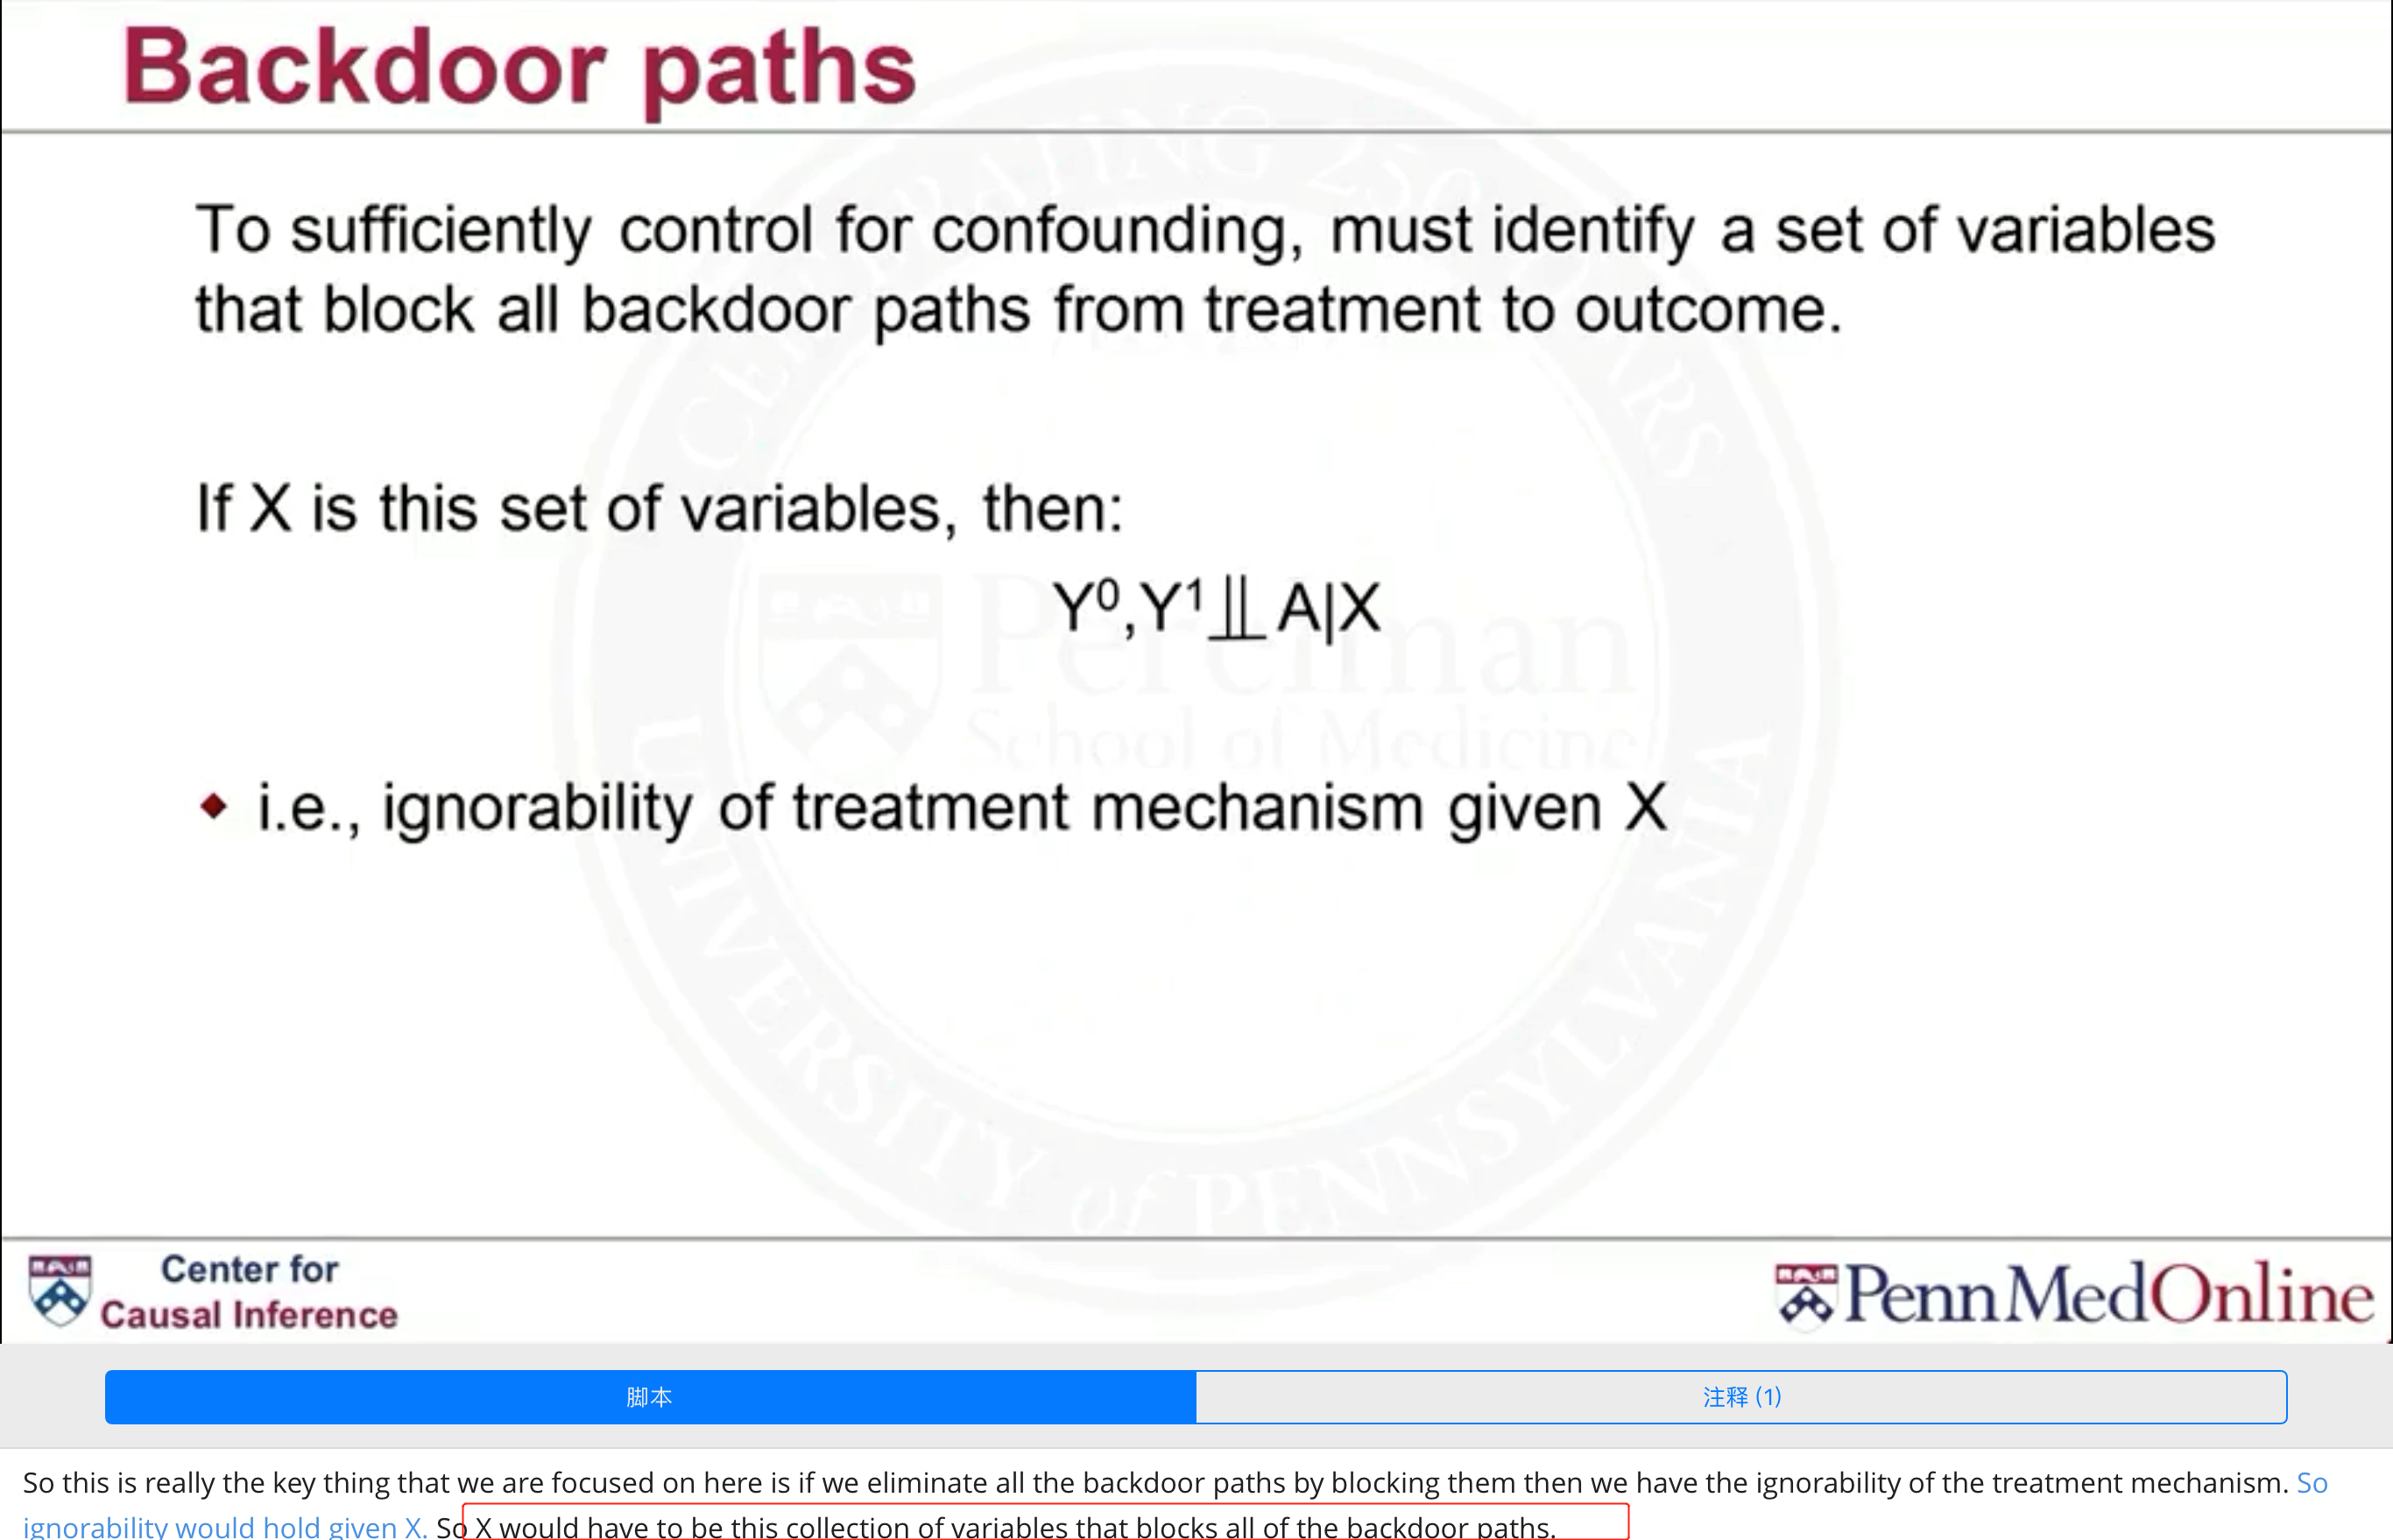
\includegraphics[width=0.8\textwidth]{figure/whyblockbackdoor.png}
	\caption{Why block Backdoor path?}
	\label{whyblockbackdoor}
    \end{figure}


\section{Backdoor path criterion}
\noindent {\bfseries Outline:}\\
1. Backdoor criterion.\\
2. When a set of variables is sufficient to control confounding?

\subsection{Backdoor path criterion}
A set of variables X is sufficient to control for confounding if:
\begin{itemize}
	\item it blocks all backdoor paths from treatment to the outcome.
	\item it does not include any descendants of treatment.
\end{itemize}
This is the {\color{red} backdoor path criterion.} 满足backdoor path criterion的变量集是{\color{red}不唯一的
}

\subsection{Examples of how to find X that are sufficient to control for confounding}
{\bfseries Example 1:}在Fig.\ref{bkdrcrtex1}中,有3个变量集满足backdoor path criterion,通常我们选择变量少的集合,比如${V}$和${W}$.
	\begin{figure}[htbp]
	\setlength{\abovecaptionskip}{0pt}     %调整图片标题与图距离
	\setlength{\belowcaptionskip}{10pt}
	\vspace{-0cm}  %调整图片与上文的垂直距离
	\setlength{\abovecaptionskip}{-0cm}   %调整图片标题与图距离
	\setlength{\belowcaptionskip}{-0cm}   %调整图片标题与下文距离
	\centering
	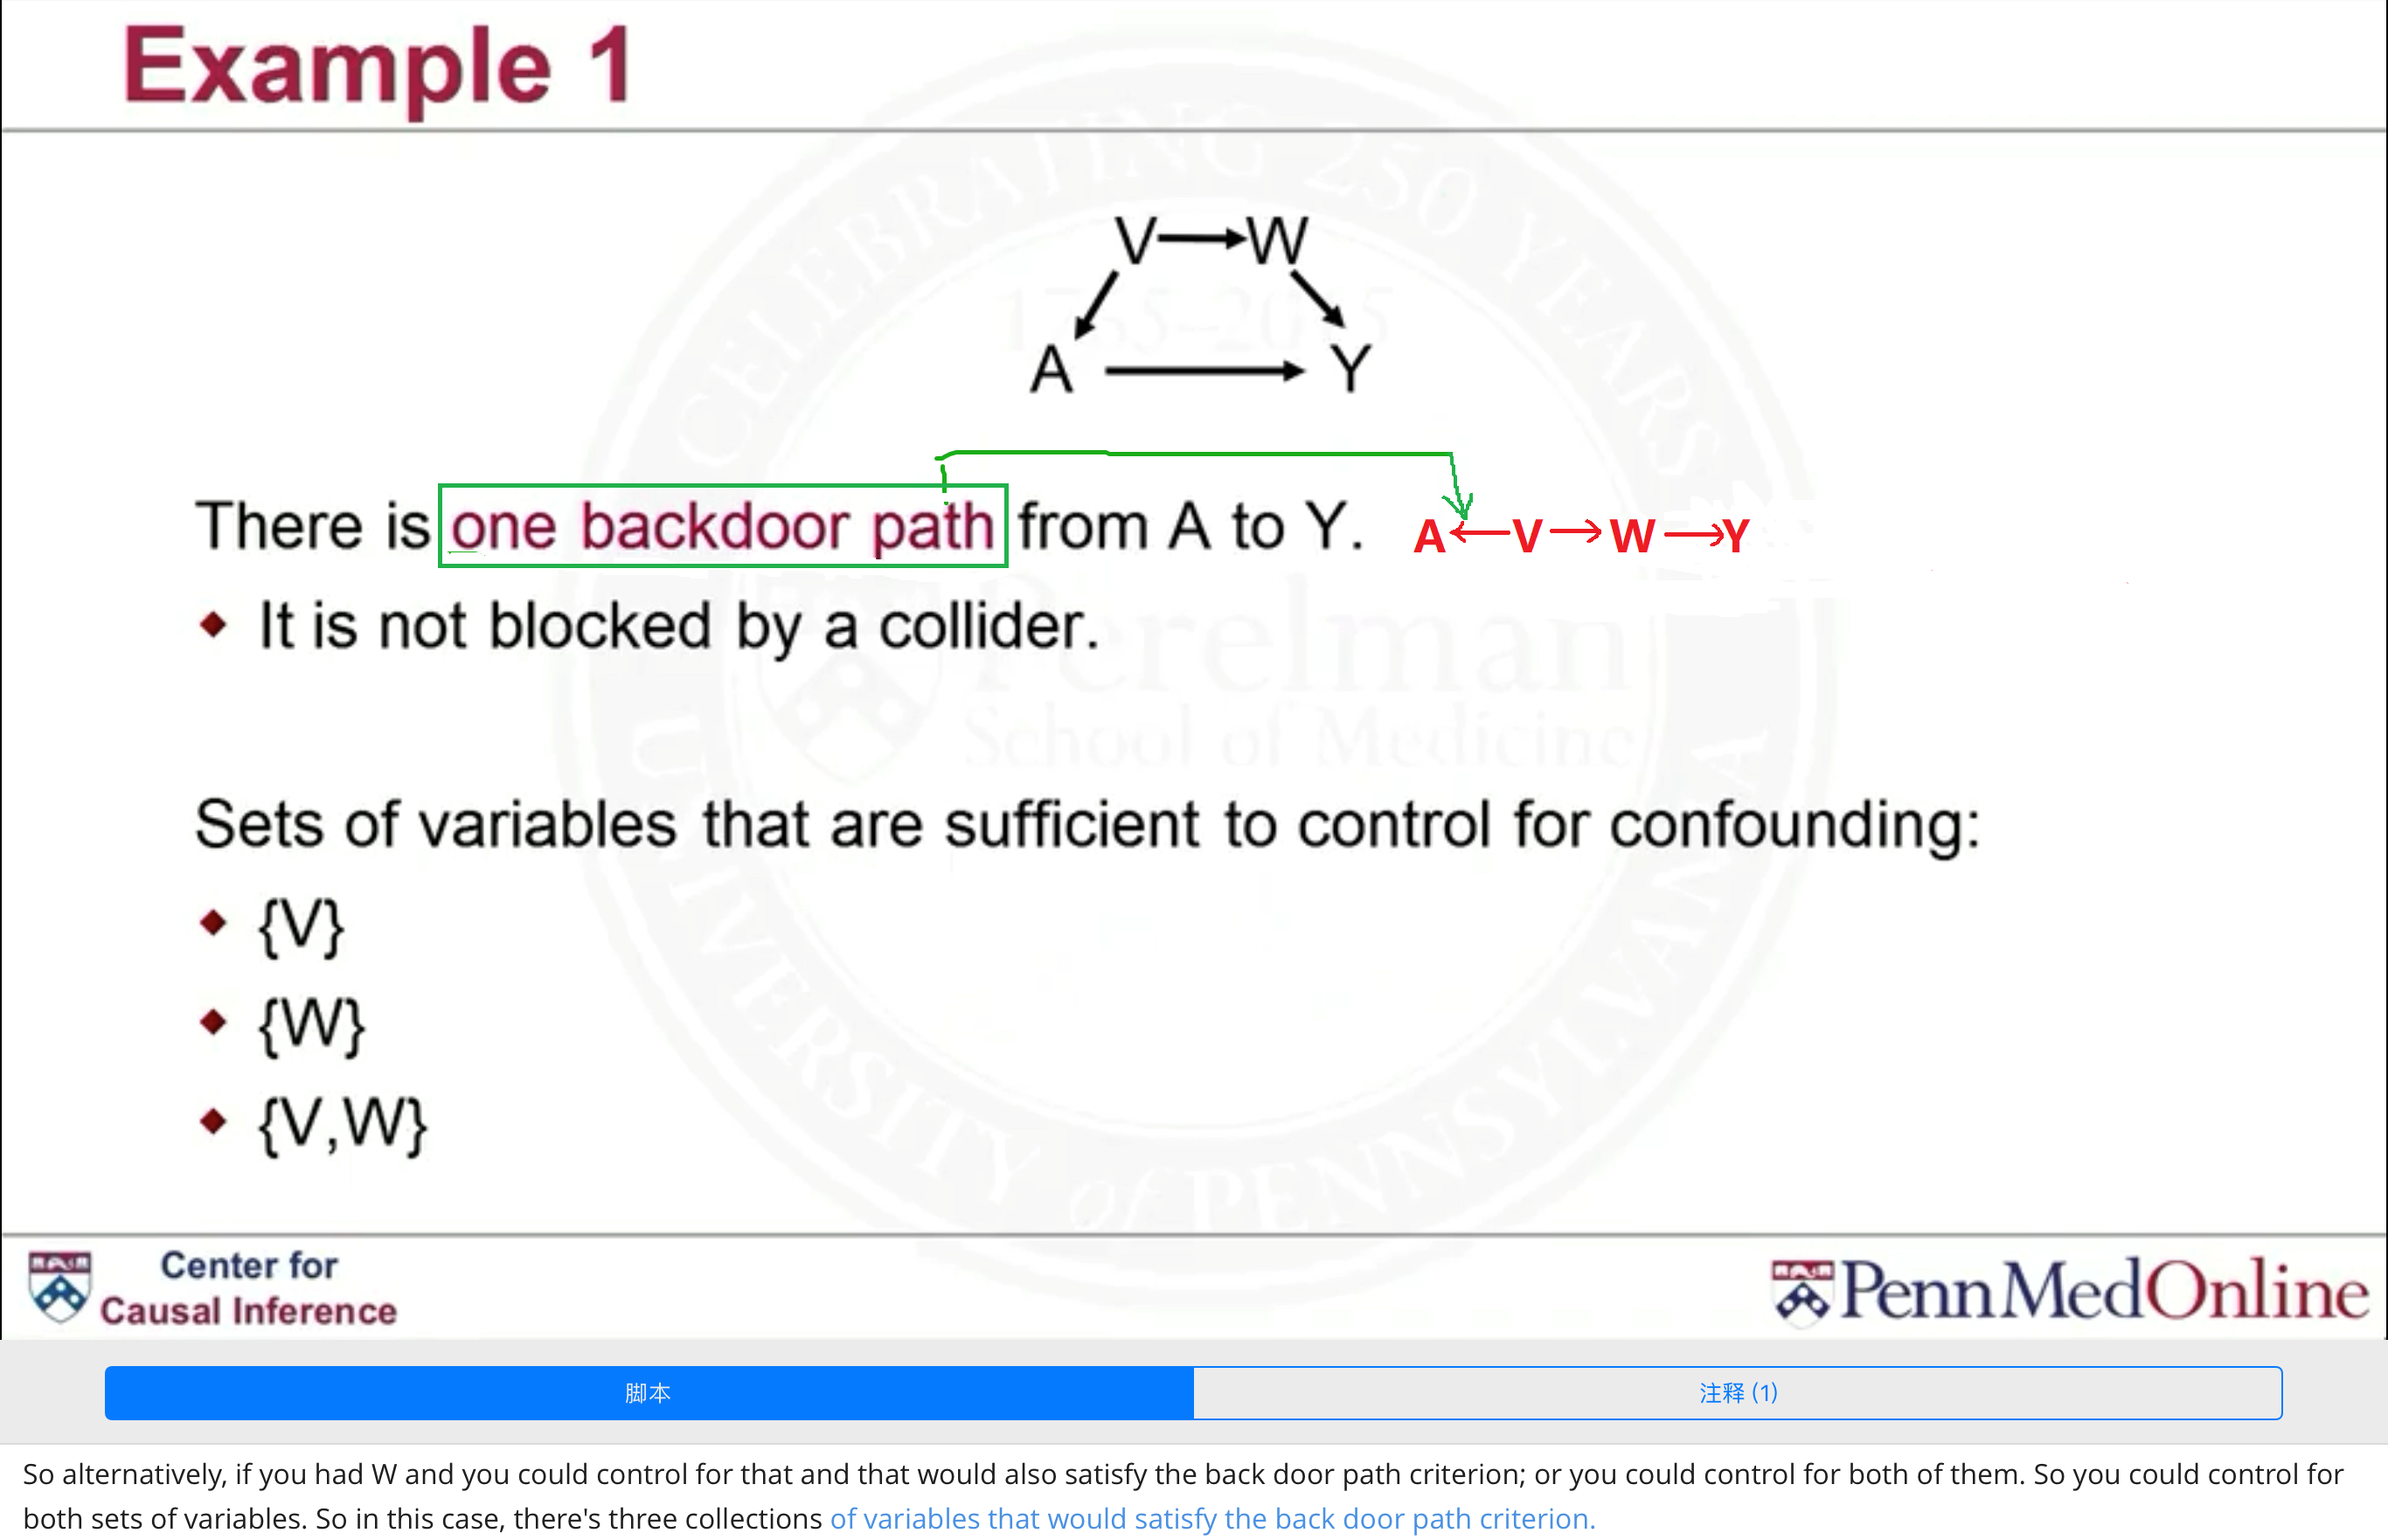
\includegraphics[width=0.8\textwidth]{figure/bkdrcrtex1.png}
	\caption{Example of backdoor path criterion(1)}
	\label{bkdrcrtex1}
\end{figure}


{\bfseries Example 2:} 
\begin{figure}[htbp]
	\setlength{\abovecaptionskip}{0pt}     %调整图片标题与图距离
	\setlength{\belowcaptionskip}{10pt}
	\vspace{-0cm}  %调整图片与上文的垂直距离
	\setlength{\abovecaptionskip}{-0cm}   %调整图片标题与图距离
	\setlength{\belowcaptionskip}{-0cm}   %调整图片标题与下文距离
	\centering
	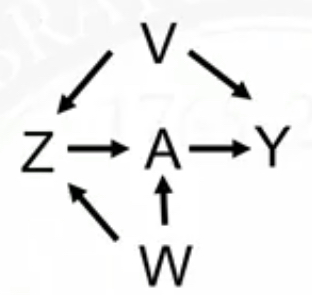
\includegraphics[width=0.2\textwidth]{figure/bckdrcrtex2.png}
	\caption{Example of backdoor path criterion((2)}
	\label{bckdrcrtex2}
\end{figure}
在Fig.\ref{bckdrcrtex2}中,我们可以找到两条backdoor paths from A to Y. 解答步骤在Fig.\ref{answerbckdrcrtex2}中详细给出.
\begin{figure}[htbp]
	\setlength{\abovecaptionskip}{0pt}     %调整图片标题与图距离
	\setlength{\belowcaptionskip}{10pt}
	\vspace{-0cm}  %调整图片与上文的垂直距离
	\setlength{\abovecaptionskip}{-0cm}   %调整图片标题与图距离
	\setlength{\belowcaptionskip}{-0cm}   %调整图片标题与下文距离
	\centering
	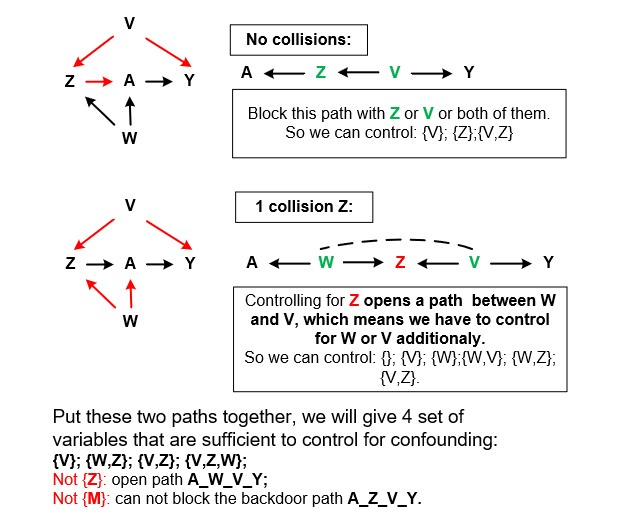
\includegraphics[width=0.8\textwidth]{figure/answerbckdrcrtex2.png}
	\caption{Solution step of example(2)}
	\label{answerbckdrcrtex2}
\end{figure}
在这个例子中,需要说明的是为什么在backdoor path:A $\longleftarrow$ W $\longrightarrow$ Z $\longleftarrow$ V $\longrightarrow$ Y上,不控制variables也可以?  这是因为这条backdoor path包含一个collider Z, 所以这条backdoor path本身就是blocked的,可以不用control任何一个变量.


{\bfseries Example 2:} 
Now we give another complicated example in Fig.\ref{bckdrcrtex3}.
\begin{figure}[h]
	\setlength{\abovecaptionskip}{0pt}     %调整图片标题与图距离
	\setlength{\belowcaptionskip}{10pt}
	\vspace{-0cm}  %调整图片与上文的垂直距离
	\setlength{\abovecaptionskip}{-0cm}   %调整图片标题与图距离
	\setlength{\belowcaptionskip}{-0cm}   %调整图片标题与下文距离
	\centering
	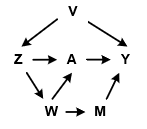
\includegraphics[width=0.2\textwidth]{figure/bckdrcrtex3.png}
	\caption{Example of backdoor path criterion((2)}
	\label{bckdrcrtex3}
\end{figure}
解答的步骤如Fig.\ref{answerbckdrcrtex3}所示. 结合所有的backdoor paths,我们可以总结出以下的sets of variables that are sufficient to control for confounding:

\begin{figure}[htbp]
	\setlength{\abovecaptionskip}{0pt}     %调整图片标题与图距离
	\setlength{\belowcaptionskip}{10pt}
	\vspace{-0cm}  %调整图片与上文的垂直距离
	\setlength{\abovecaptionskip}{-0cm}   %调整图片标题与图距离
	\setlength{\belowcaptionskip}{-0cm}   %调整图片标题与下文距离
	\centering
	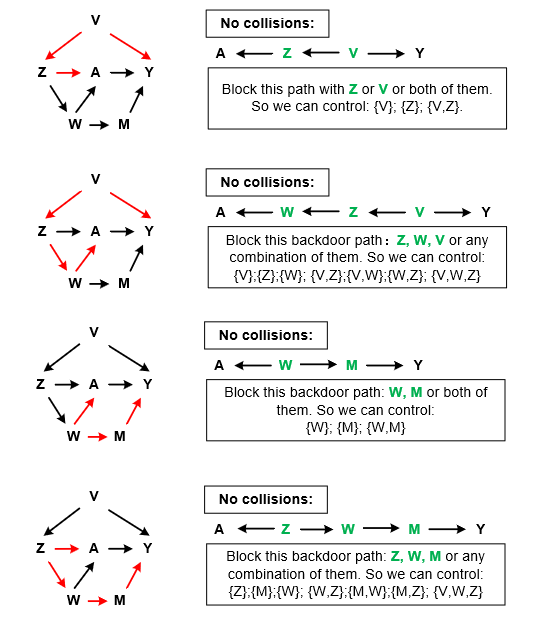
\includegraphics[width=0.8\textwidth]{figure/answerbckdrcrtex3.png}
	\caption{Solution step of example(3)}
	\label{answerbckdrcrtex3}
\end{figure}
Put these two paths together, we will give   sets of variables that are sufficient to control for confounding:$\{V,M\},\{V,W\},\{Z,W\},\{Z,M\}; \{V,W,M\},\{V,Z,M\},\{V,Z,W\}; \{V,Z,W,M\}$.


\subsection{Conclusion}
上面所给出的例子都是基于正确的DAG,有了正确的DAG,我们才知道应该控制哪些变量. 问题在于:在实际问题中我们一开始并不知道真实的DAG是什么样子的. 此时如何构造DAG?进一步,如果构造的DAG不一定正确该怎么办?

我们关注的问题是:在DAG有小幅变动的情况下,confoundr control仍然有效. 或者说:If the DAG looks slightly different, can we still sufficiently control for confounding? 
\begin{figure}[htbp]
	\setlength{\abovecaptionskip}{0pt}     %调整图片标题与图距离
	\setlength{\belowcaptionskip}{10pt}
	\vspace{-0cm}  %调整图片与上文的垂直距离
	\setlength{\abovecaptionskip}{-0cm}   %调整图片标题与图距离
	\setlength{\belowcaptionskip}{-0cm}   %调整图片标题与下文距离
	\centering
	
\includegraphics[width=0.8\textwidth]{figure/conclusionbdc.jpg}
	\caption{Conclusion of backdoor path criterion}
	\label{conclusionbdc}
\end{figure}

\section{Disjunctive cause criterion}
\noindent {\bfseries Outline:}\\
1. Disjunctive cause criterion. \\
2. The relationship between \r{disjunctive cause criterion} and \r{backdoor path criterion.} \\
3. {\bfseries Comparasion} of \r{pre-treatment covariates} and \r{disjunctive cause criterion.}

\subsection{Disjunctive cause criterion}
{\bfseries Disjunctive cause criterion: } Control for all(observed) causes of the exposure, the outcome, or both. This criterion was put forward to choose variables to control for(VanderWeele 2011).

\paragraph{The advantage of disjunctive cause criterion.} One \r{has no need to know the whole graph}, usually we can not know the whole graph. Instead, we \r{only need to identify the variables that affect exposure or outcome.}

\subsection{Property}
The property of disjunctive cause criterion shows its  relationship with \r{backdoor path criterion.}
\begin{thm}
	If there is a set of variables that satisfy the backdoor path criterion, then the variables selected based on the disjunctive cause criterion will be sufficient to control for confounding.
\end{thm}

这个定理告诉我们,如果存在满足backdoor path criterion的观测变量集,那么基于disjunctive cause criterion选择的变量将足够控制confounding.

\subsection{Pre-treatment covariates}
Here we don't know what the DAG is, but we might have some information about observed variables.  

One strategy is using all observed pre-treatment covariates. 

\begin{ex}
	\label{exdcc1}
	Observed pre-treatment variables:${M,W,V}$;
	Unobserved pre-treatment variables: ${U_1,U_2}$;
	Suppose we know that W and V are the causes of A, Y or both. M is not a cuase of either A or Y. Fig.\ref{exdcc} is the causal graph of this example.
 Then compare 2 methods for selecting variables to control: 
 \begin{itemize}
 	\item Use all observed pre-treatment covariate: ${M,W,V}$. The set of variables satisfies the backdoor path criterion.
 	\item Use variables based on dcc: ${W,V}$. The set of variables satisfies the backdoor path criterion.
 \end{itemize}

在这种情况下,两种方法得到的set of variables are sufficient to control for confounding.
\end{ex}

\begin{figure}[htbp]
	\setlength{\abovecaptionskip}{0pt}     %调整图片标题与图距离
	\setlength{\belowcaptionskip}{10pt}
	\vspace{-0cm}  %调整图片与上文的垂直距离
	\setlength{\abovecaptionskip}{-0cm}   %调整图片标题与图距离
	\setlength{\belowcaptionskip}{-0cm}   %调整图片标题与下文距离
	\centering
	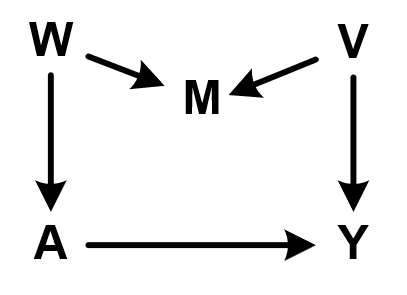
\includegraphics[width=0.2\textwidth]{figure/exdcc.png}
	\caption{Hypothetical Dag 2}
	\label{exdcc}
\end{figure}

需要强调的是,像{\bfseries Example\ref{exdcc1}}这样,两种准则都适用的情况并不常见,下面我们将给出两个例子,说明当观测变量刚好是未观测变量的collider时,控制pre-treatment变量和Disjunctive cause criterion将会失效. 
\begin{figure}[htbp]
	\setlength{\abovecaptionskip}{0pt}     %调整图片标题与图距离
	\setlength{\belowcaptionskip}{10pt}
	\vspace{-0cm}  %调整图片与上文的垂直距离
	\setlength{\abovecaptionskip}{-0cm}   %调整图片标题与图距离
	\setlength{\belowcaptionskip}{-0cm}   %调整图片标题与下文距离
	\centering
	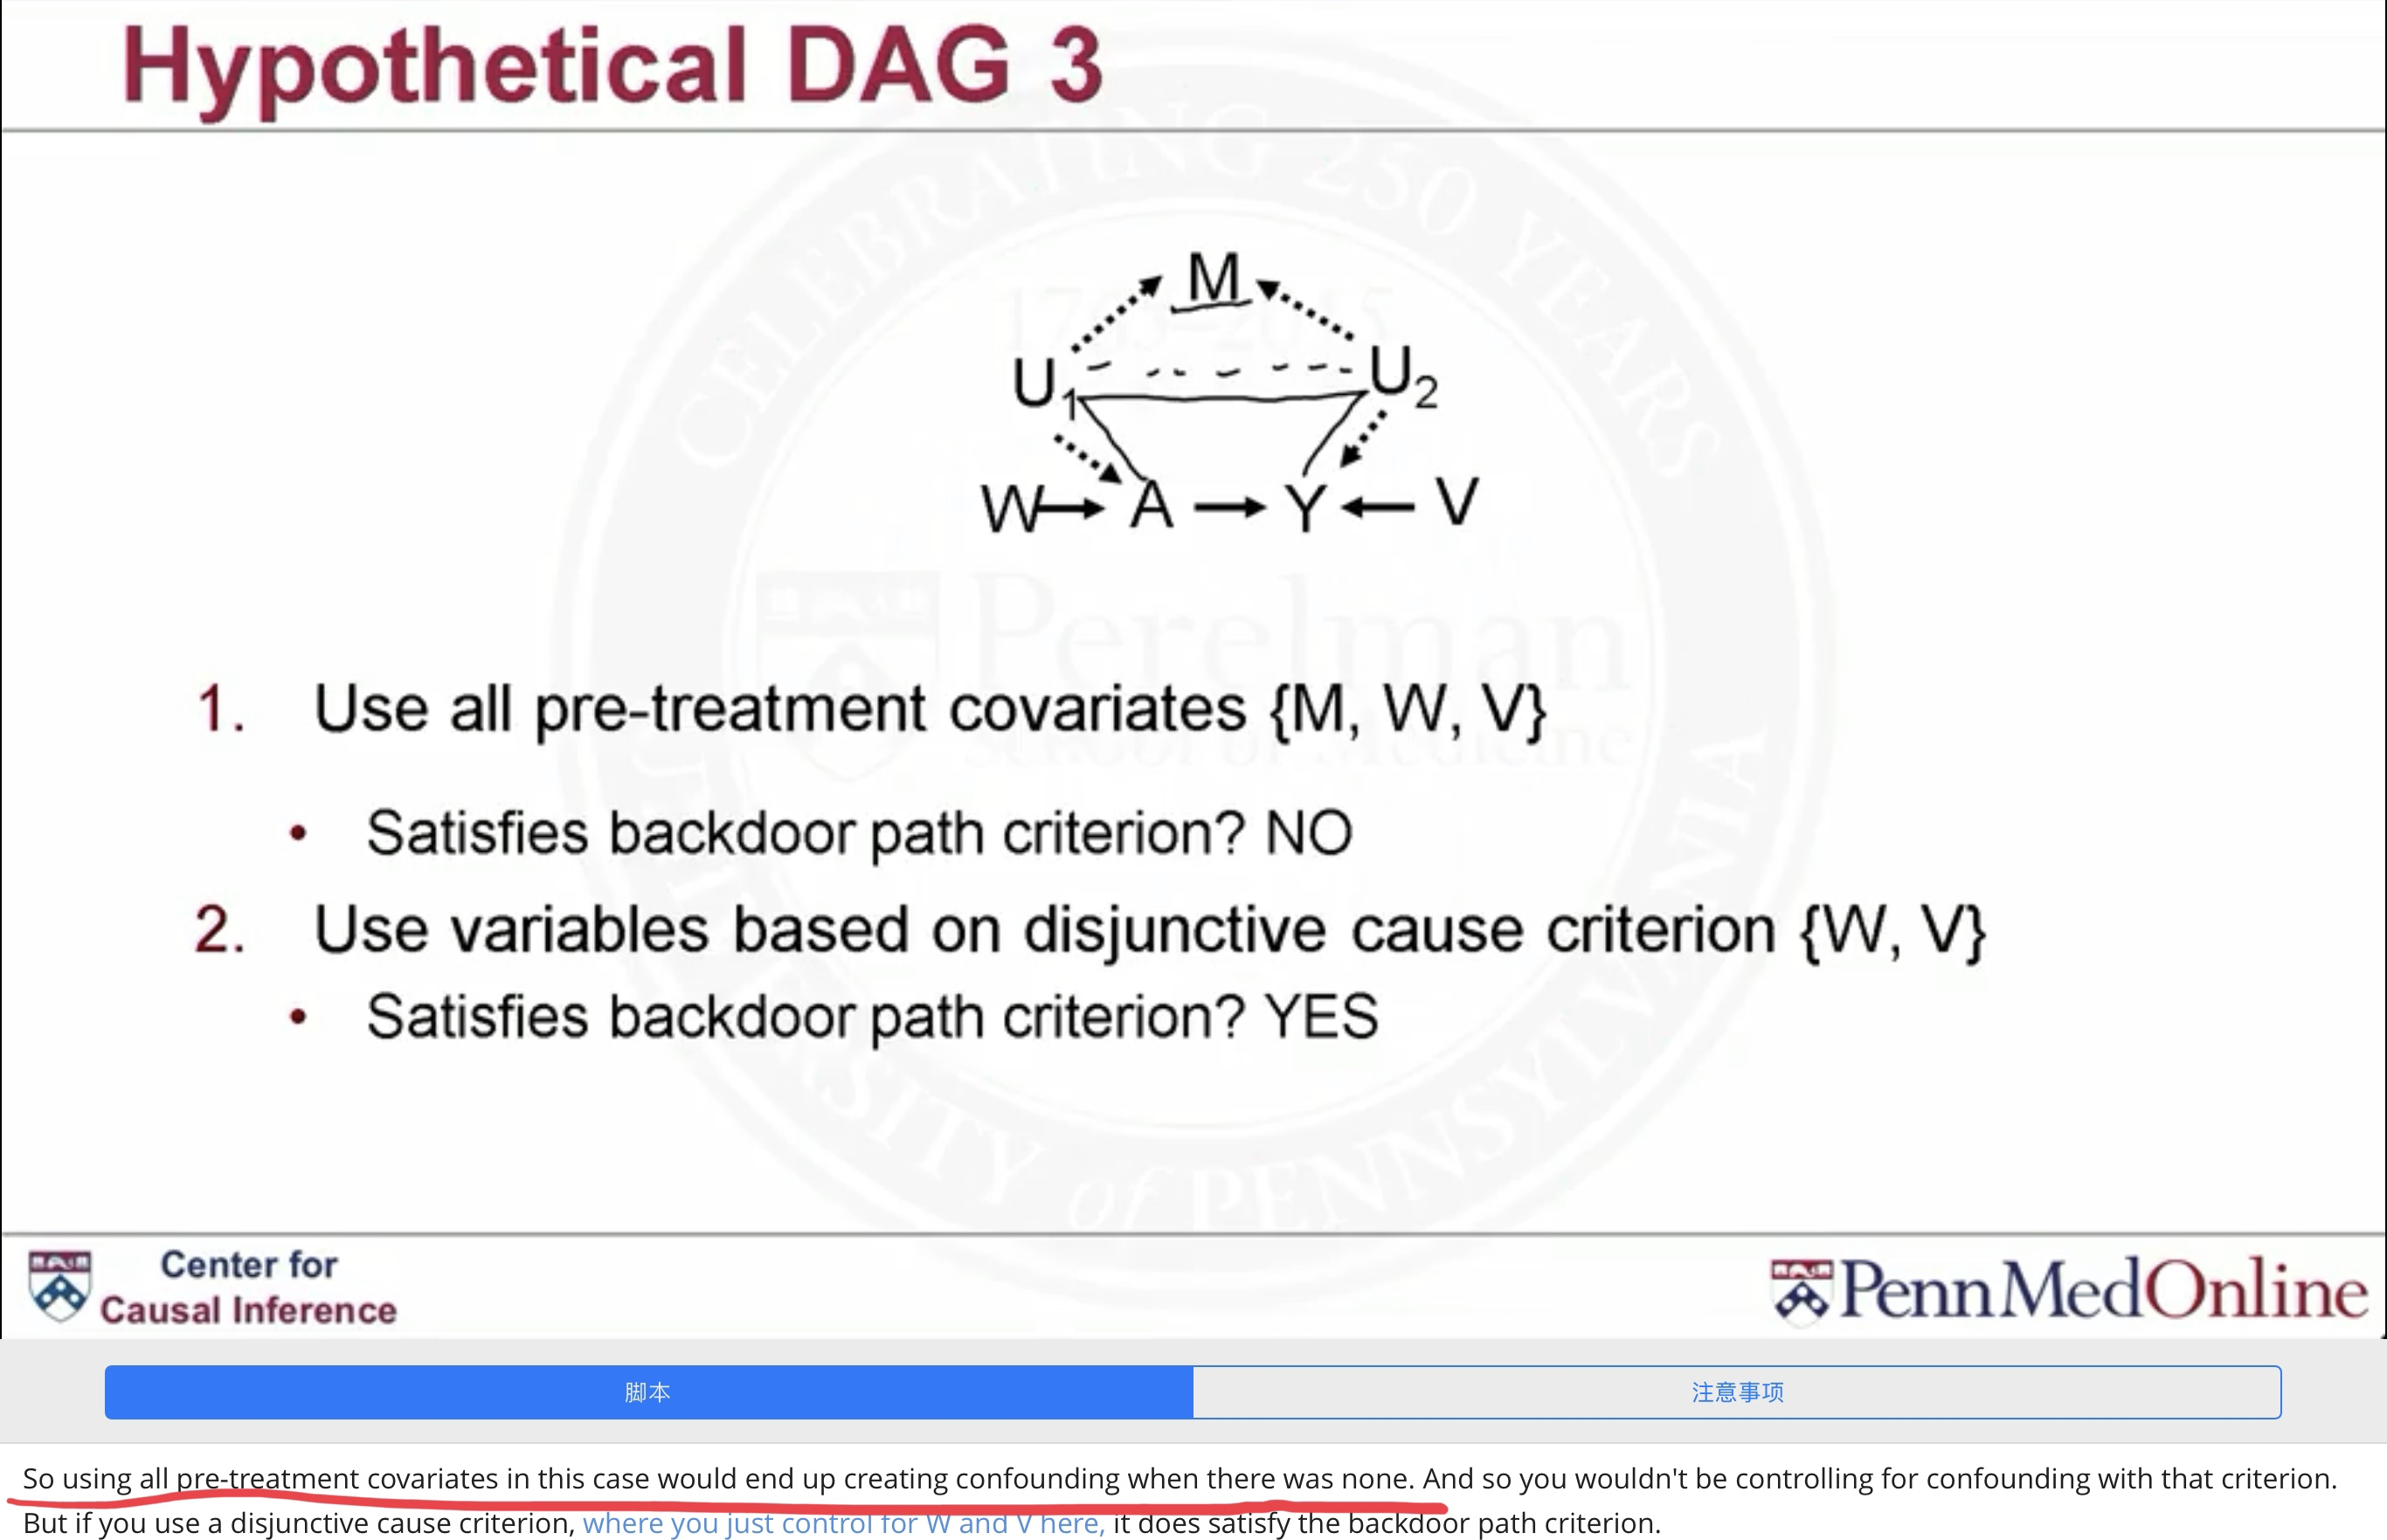
\includegraphics[width=0.6\textwidth]{figure/dccdag3.jpg}
	\caption{Hypothetical Dag 3}
	\label{dccdag3}
\end{figure}
	
\begin{figure}[htbp]
	\setlength{\abovecaptionskip}{0pt}     %调整图片标题与图距离
	\setlength{\belowcaptionskip}{10pt}
	\vspace{-0cm}  %调整图片与上文的垂直距离
	\setlength{\abovecaptionskip}{-0cm}   %调整图片标题与图距离
	\setlength{\belowcaptionskip}{-0cm}   %调整图片标题与下文距离
	\centering
	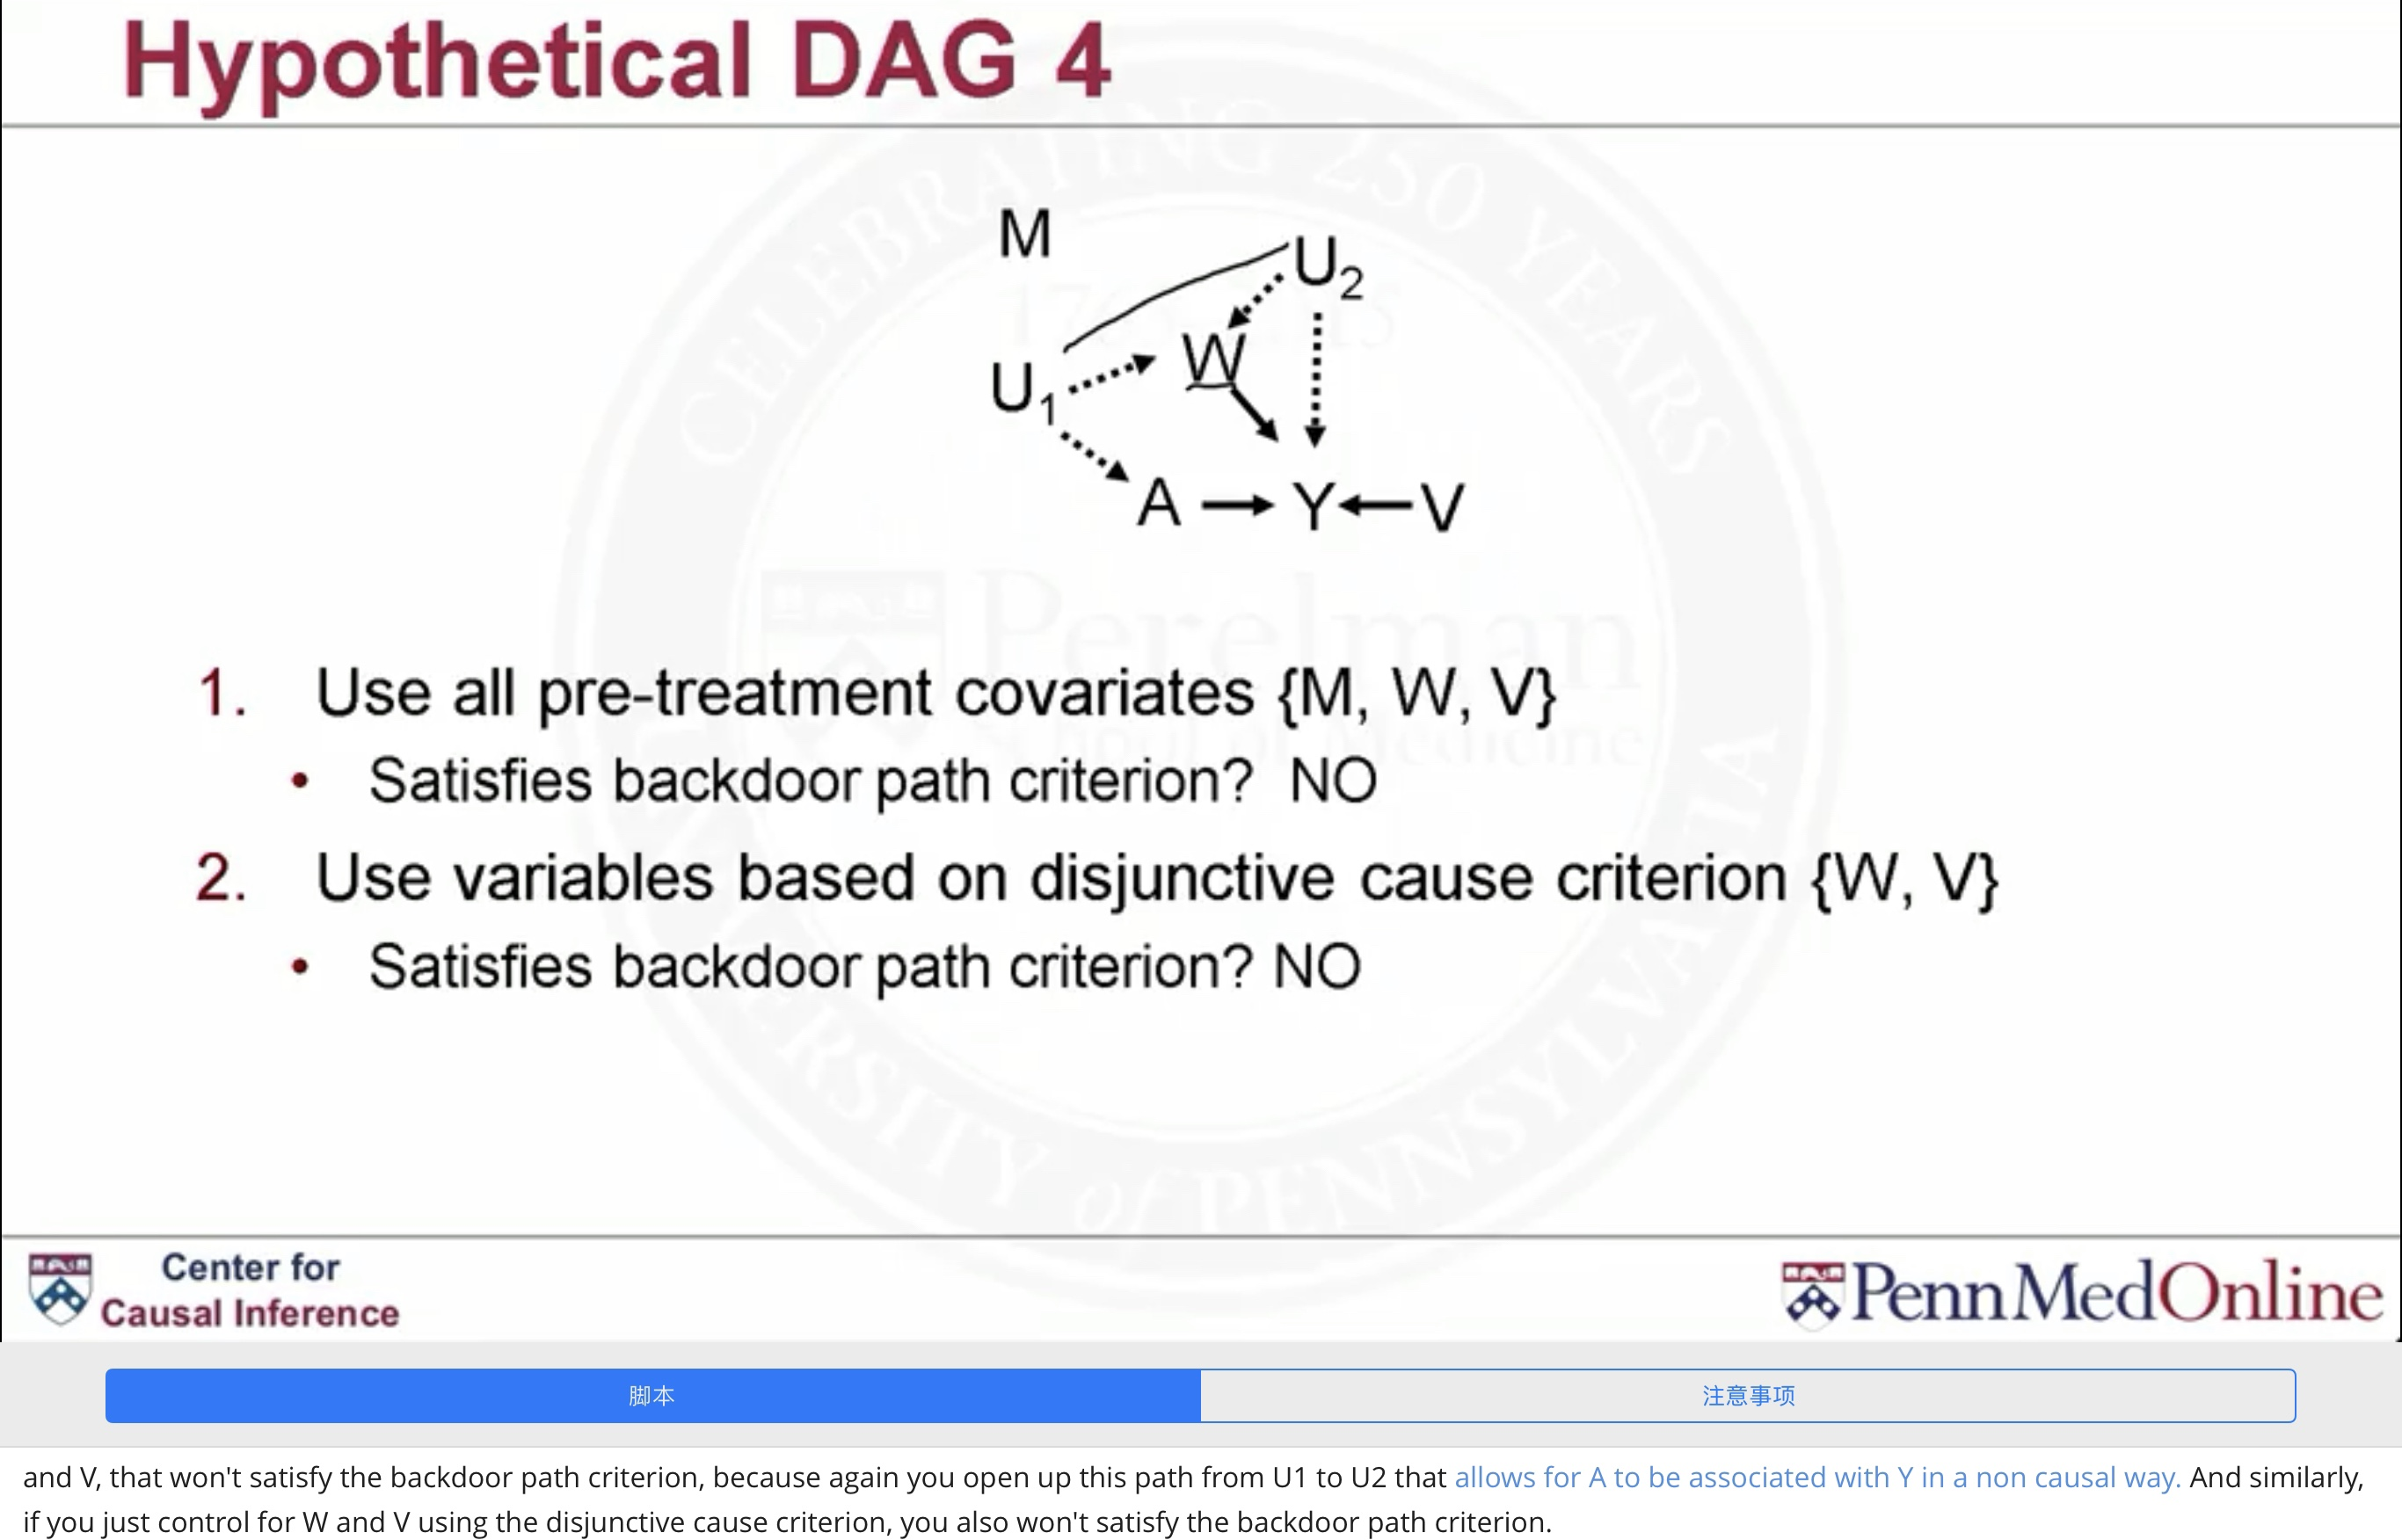
\includegraphics[width=0.6\textwidth]{figure/dccdag4.jpg}
	\caption{Hypothetical Dag 4}
	\label{dccdag4}
\end{figure}	

















    \chapter{Propensity Score Matching}

\section{Observational studies}
\noindent {\bfseries Outline}:\\
1. Randomized trial.\\
2. The difference between randomized trials and observational studies.
\begin{itemize}
	\item[$\blacksquare$] Classic confounding setting.
	\item[$\blacksquare$] Ignorability assumption.
	\item[$\blacksquare$] Causal graphs of two situations.
	\item[$\blacksquare$] Good properties in randomized trials.
	\item[$\blacksquare$] Why not always randomize?
\end{itemize}

\noindent 3. How to control for confounding?

Matching. {\color{orange}The basic idea} is to control for confounding, and making the observational studies be likely to the randomized trials.

\noindent 4. Advantage of Matching.

\subsection{Randomized trials}
\paragraph{In a randomized trial, treatment is randomly assigned.} 在随机实验中,每个subject的处理都是随机分配的. 因此处理A的分配与covariates X是无关的,可以移除DAG中X到A的边. 

\subsection{Randomized trail and obsevational studies}
The difference between randomized trail and obsevational studies is shown in Fig.\ref{rmtrail}.
\begin{figure}[htbp]
	\setlength{\abovecaptionskip}{0pt}     %调整图片标题与图距离
	\setlength{\belowcaptionskip}{10pt}
	\vspace{-0cm}  %调整图片与上文的垂直距离
	\setlength{\abovecaptionskip}{-0cm}   %调整图片标题与图距离
	\setlength{\belowcaptionskip}{-0cm}   %调整图片标题与下文距离
	\centering
	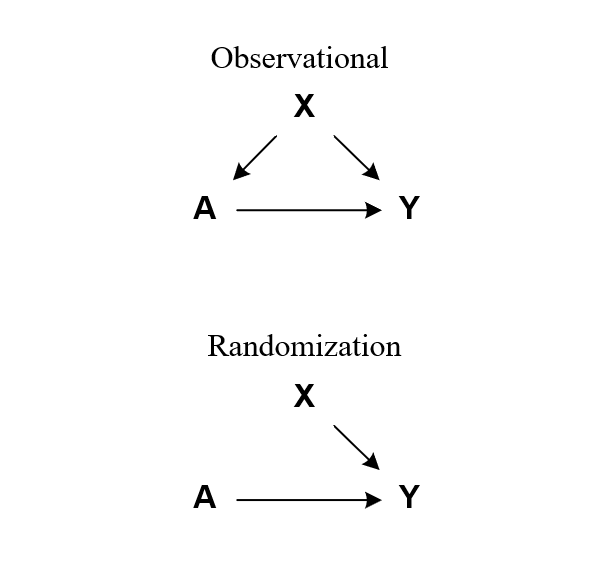
\includegraphics[width=0.6\textwidth]{figure/rmtrail.png}
	\caption{Randomized trail}
	\label{rmtrail}
\end{figure}

在Randomized trail中不存在backdoor path from A to Y. 但是在observation中仍然存在. 我们想要做的就是令observation接近于randomization,消除X对A的影响.

\paragraph{Randomization的作用: }通过随机化分配A,消除X对A的影响.
\paragraph{Good property in randomized trial.}The distribution of pre-treatment variables X will be the same in both treatment groups. e.g. {\color{red} Covariate balance.}

\paragraph{Balance is the distribution of these covariates to be the same in two treatment groups.}因此,如果两个treatment groups的outcome不同,不会是因为两组X的不同所导致的,而只能是处理的不同导致的. 

\subsection{Why not always randomize?}
\begin{figure}[htbp]
	\setlength{\abovecaptionskip}{0pt}     %调整图片标题与图距离
	\setlength{\belowcaptionskip}{10pt}
	\vspace{-0cm}  %调整图片与上文的垂直距离
	\setlength{\abovecaptionskip}{-0cm}   %调整图片标题与图距离
	\setlength{\belowcaptionskip}{-0cm}   %调整图片标题与下文距离
	\centering
	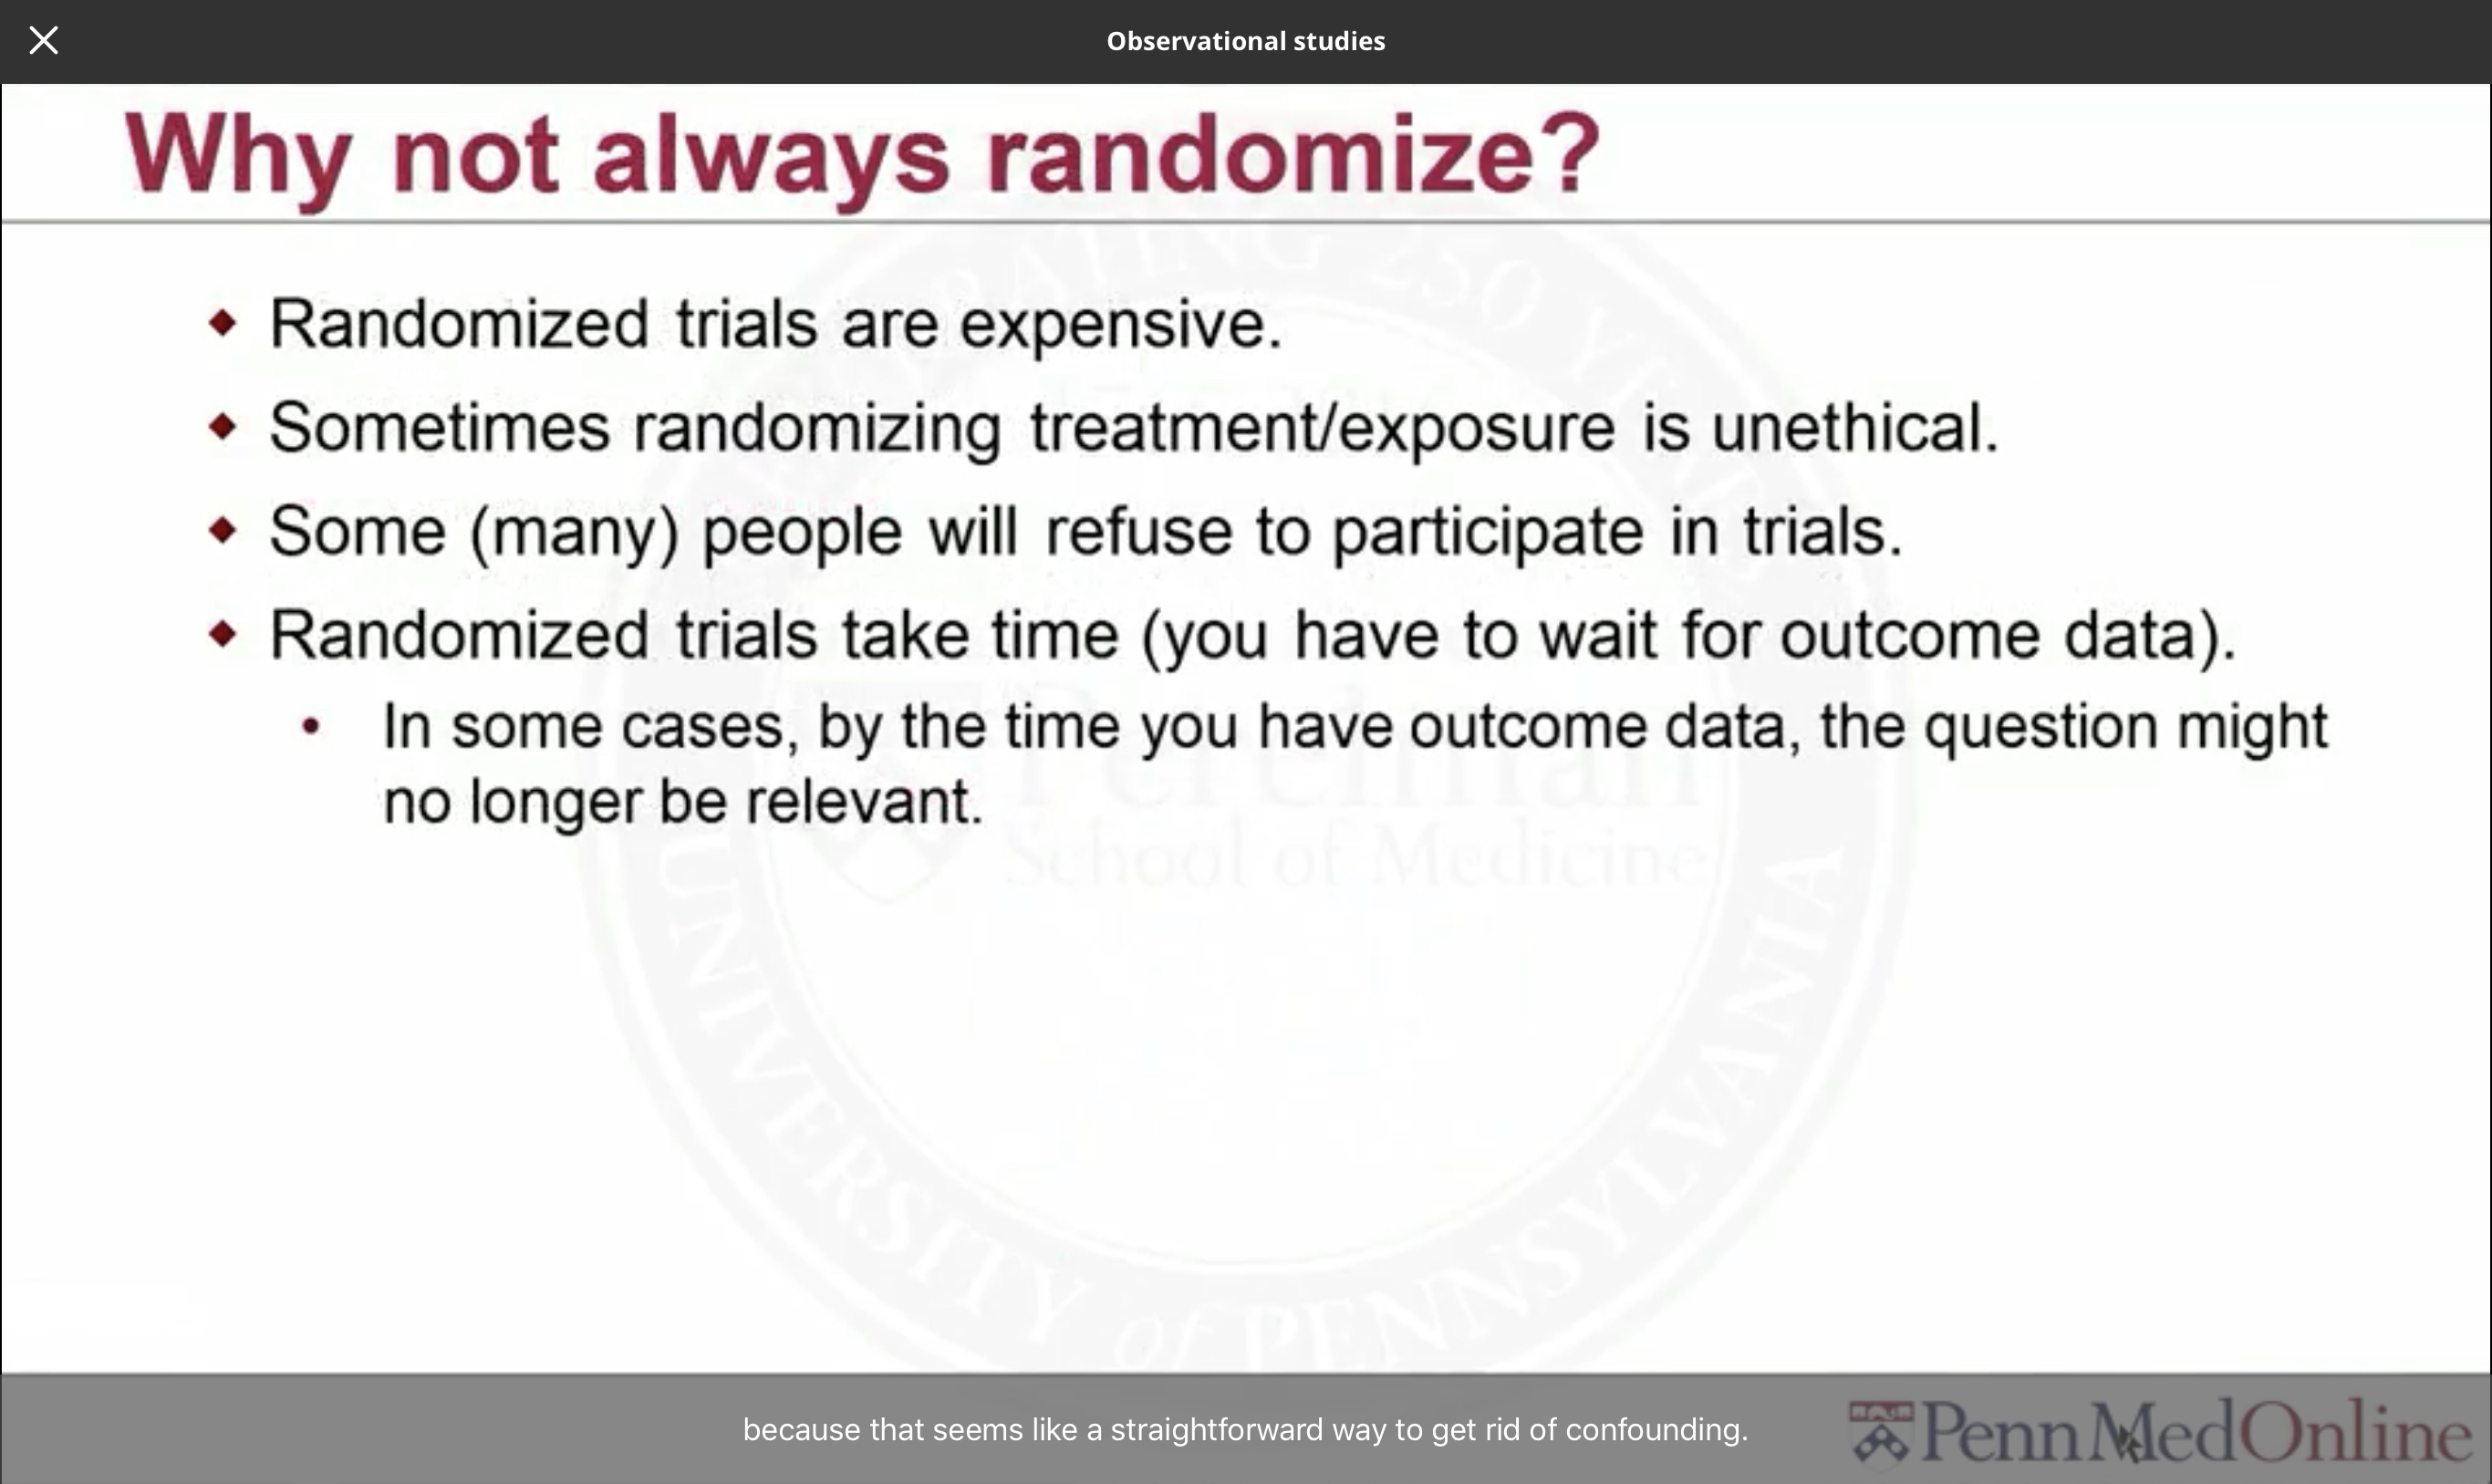
\includegraphics[width=0.8\textwidth]{figure/rmwhynot.jpg}
	\caption{Why not always randomize?}
	\label{rmwhynot}
\end{figure}

\subsection{Recall}
\noindent 1. Classic confounding setting
\begin{itemize}
	\item a set of variable $X$.
	\item $X \rightarrow A$.
	\item $X \rightarrow Y$.
\end{itemize}

在下面两个条件下,控制$X$ is sufficient to control for confounding:
\begin{enumerate}[itemindent=2em,label=(\arabic*)] 
	\item Disjunctive cause criterion.
	\item Backdoor path criterion.
\end{enumerate}

\noindent 2. Ignorability assumption
\begin{equation}
Y^0,Y^1 \perp A|X.
\end{equation}

在给定X后,outcome与处理独立.可以理解为,在X相同的样本中,outcome与是否处理是独立的.


\section{Overview of Matching}
\noindent {\bfseries Outline}:\\
1. Stochastic balance and Fine balance.

\subsection{Single Covariate}
假设只有一个Covariate,可以通过matching达到treated组和control组的perfect match.
\begin{enumerate}[label=(\arabic*)]
	\item Match each treated subject to control subject.
	
	\item Find the best matches and get rid of the subjects who were't matched. 在上一节也说过,我们要去掉那些“have no chance to get another treat"的subjects.
\end{enumerate}

通过Matching,covariate的各取值在treated和control组中的比例都相同,可以达到精准的匹配.

\subsection{Many Covariates}
当有多个covariates的时候,我们不能对所有的covariates都进行perfect match. 即使是在randomized trials的情况下,给定一个treated subject,也可能不存在达成perfect match的single control subject.
此时,randomized trial达到的是一种covariates分布的组间“平衡”,称为{\color{red}{“Stochastic balance”}}.

\begin{ex}
In this example,We have two covaraites:age and gender. There are two subjects in treated group: male aged 56 and female aged 47. \\
\begin{note}
	{\color{orange} \quad Start in treated group, and find people in the control group who are like them.} 
\end{note} 
现在我们在Control group中找一个male subject whose age is similar to 56. 然后再在Control group中找一个female subject whose age is similar to 47. 如Fig.\ref{twocovariates}所示.
\end{ex}

\begin{figure}
	\setlength{\abovecaptionskip}{0pt}     %调整图片标题与图距离
	\setlength{\belowcaptionskip}{10pt}
	\vspace{-0cm}  %调整图片与上文的垂直距离
	\setlength{\abovecaptionskip}{-0cm}   %调整图片标题与图距离
	\setlength{\belowcaptionskip}{-0cm}   %调整图片标题与下文距离
	\centering
	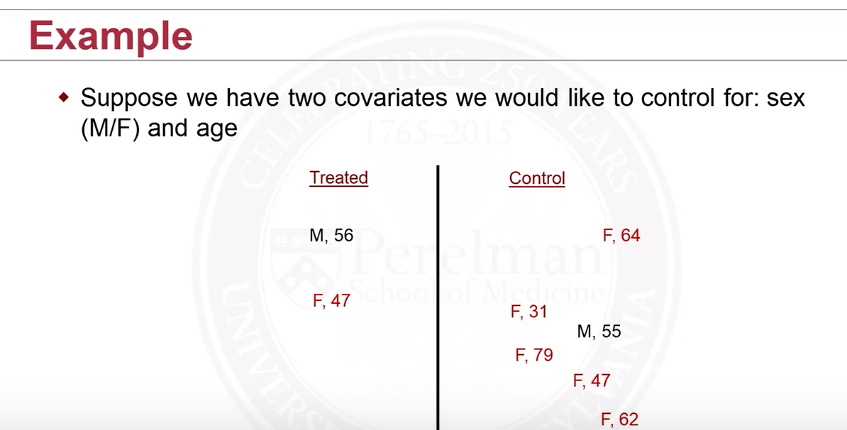
\includegraphics[width=0.8\textwidth]{figure/twocovariates.png}
	\caption{Example:two covariates matching}
	\label{twocovariates}
\end{figure}
在这个过程中,我们是在令control group中的covariates的分布与treated population近似,本质上是求"causal effect of treatment on the treated".

\noindent {\bfseries Remember:}\\
在Matching的过程中,\hl {If we begin with the treated group, and then try to find controls that are good matches for them, you're essentially making inference about the treated population.So you're estimating the "causal effect of treatment on the treated".}

\subsection{Stochastic balance:}
这是一种covariates分布的组间“balance”,“balance”是指confounders在tread group和control group中的分布是相似的. 
\begin{itemize}
   \item Matching {\color{red}{not}} exactly.
   \item Close matches and the distribution of covariates should be {\color{red}{similar}} in two groups.
\end{itemize}


\subsection{Fine balance}
有时候我们不能达到great matching,需要适当放松对matching的要求. 我们可以接受一些non-ideal matching的点,但要求treated和control group中具有the same distribution of covariates. 这种情况称为{\color{red}fine matching}.

\begin{figure}
	\setlength{\abovecaptionskip}{0pt}     %调整图片标题与图距离
	\setlength{\belowcaptionskip}{10pt}
	\vspace{-0cm}  %调整图片与上文的垂直距离
	\setlength{\abovecaptionskip}{-0cm}   %调整图片标题与图距离
	\setlength{\belowcaptionskip}{-0cm}   %调整图片标题与下文距离
	\centering
	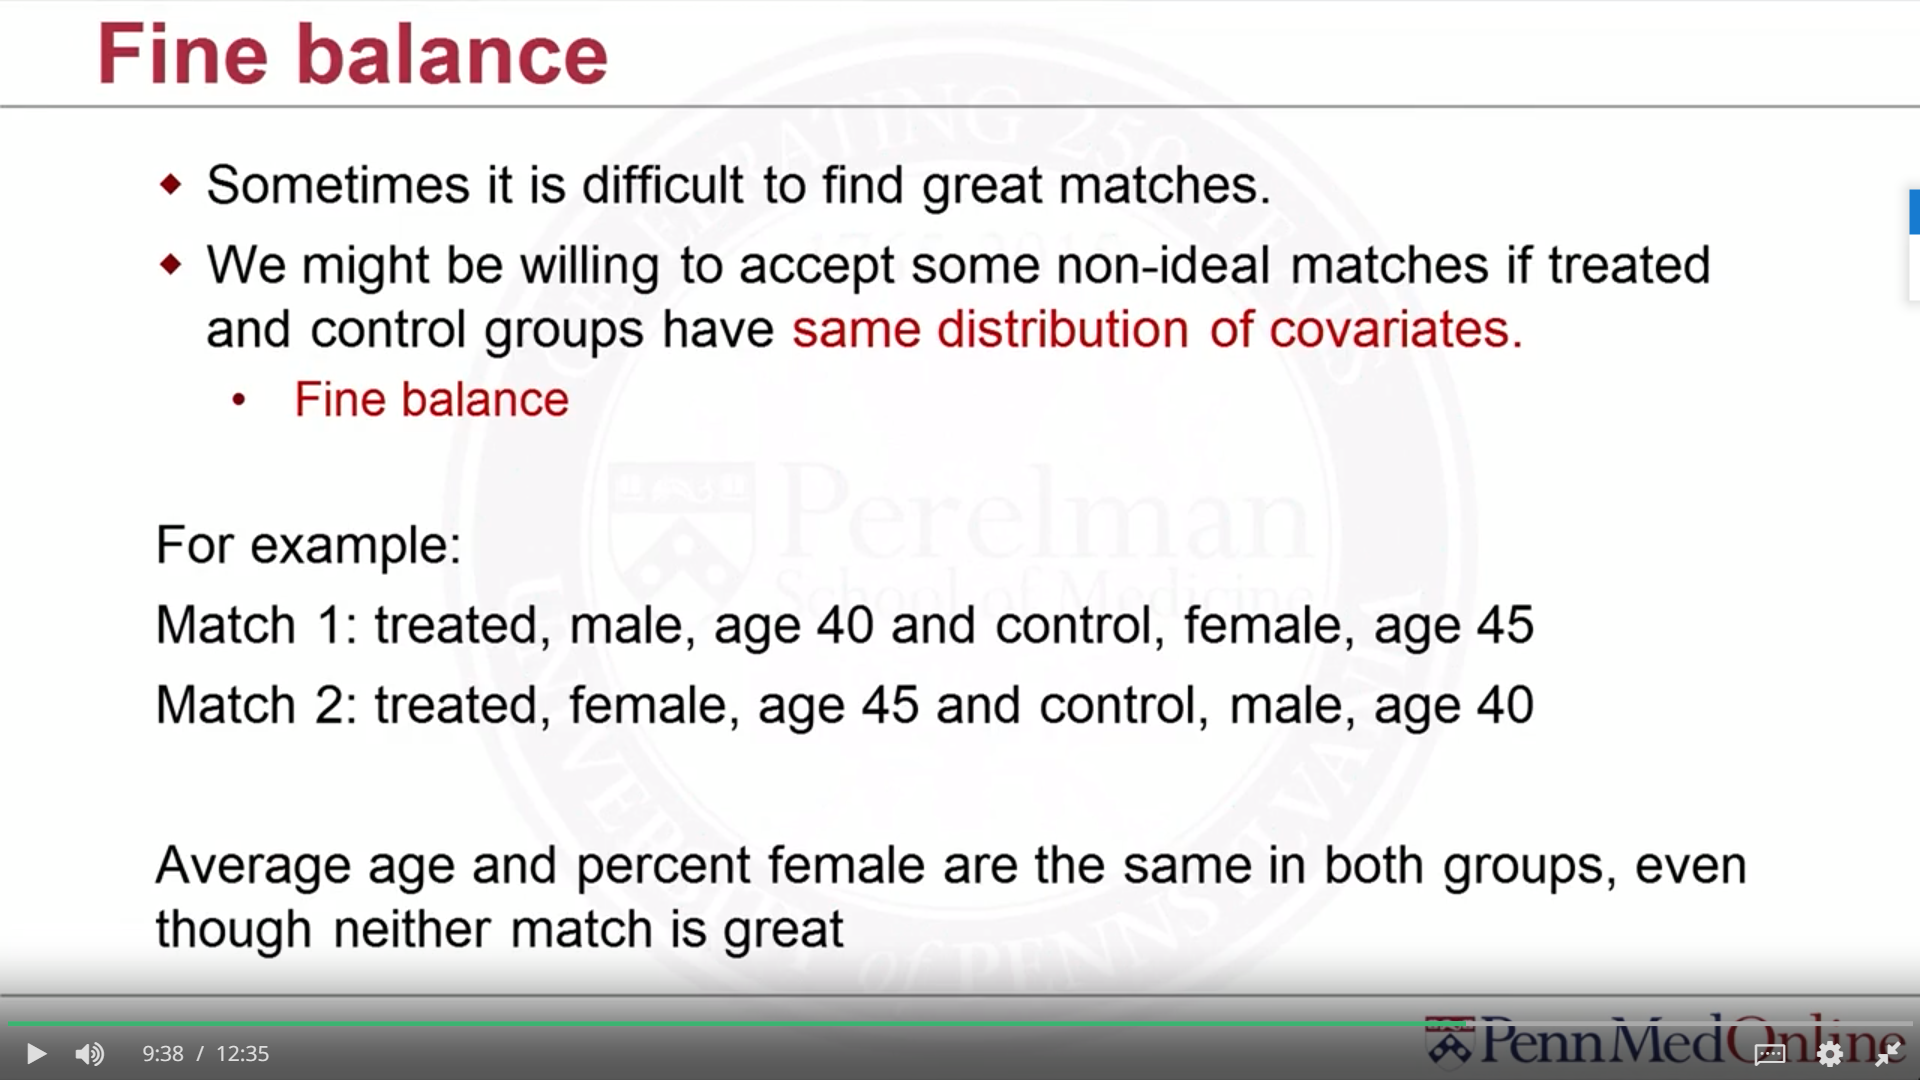
\includegraphics[width=0.8\textwidth]{figure/finebalance.png}
	\caption{Example:Fine balance}
	\label{finebalance}
\end{figure}


\subsection{Number of matches}
\begin{itemize}
	\item[$\blacktriangle$] One-to-one matching: 对于{\color{red}{每一个}}treated subject,都匹配到{\color{red}{一个}}control subject.
	
	\item[$\blacktriangle$] Many to one matching: 对于{\color{red}{每一个}}treated subject,都匹配到{\color{red}{K个}}control subject.
	\item[$\blacktriangle$] Variable matching:对于{\color{red}{每一个}}treated subject,都匹配到{\color{red}{未知个数的}}control subject.
	这依赖于我们可以找到多少对good-matches. 有时候对于一个treated subject可以找到多个good matches,那么就可以全部match上. 
\end{itemize}

当一个treated subject可以找到多个good matches时才可以使用variable matching,如果找不到多个,不要使用.

One-to-one matching的优点就是every pair is good-match. 不过它的缺点也很明显,当一个treated subject可以有多个good-macthes匹配时,只能选择一个good match,其余的controls都丢掉了,这样降低了efficiency.

\newpage \section{Greedy Matching}
\label{greedy}
{\bfseries Outline:}\\
1. What greedy (Nearest-Neighbor) matching is? How the  algorithm works?\\
2. The advantage and disadvantages of greedy matching.\\
3. Many to one matching VS pair matching. Discuss trade-off with the two approaches. \\
4. Introduce the idea of calipers.

\subsection{Set-up}
\begin{itemize}
	\item We have selected a set of pre-treatment covariates X that satisfy the ignorability assupmtion.
	\item We have calculated a distance $d_{ij}$ between each treated subject with every control subject. 计算每一个处理组的对象与每一个控制组的对象之间的距离$d_{ij}$.
\end{itemize}

\subsection{One-to-one Matching}
1. Randomly order list of treated subjects and control subjects.\\
2. {\bfseries Greedy step: find best match.} Start with the 1st treated subjects. Match to the control subject with the smallest distance.\\
3. Remove the matched control from the list of avaliable matches. 匹配过的control subject从候选controls中删掉.\\
4. Move on to the next treated subject. Match to the control with smallest distance.\\
5. Repeat steps 3 and 4 until all treated subjects being matched. \\
{\bfseries R package:MatchIt.}

\subsection{Advantage and Disadvantage}
\begin{itemize}
	\item 容易理解,原理简单.
	\item 计算速度快,计算难度小:逐个计算距离,求最小. 即使对于大型数据计算也很快.
	\item 与treated组的初始排序有关,初始排序不同,得到的匹配也不同.
	\item 不能得到全局最优解:成对的最小距离匹配并不能最小化整个total distance.
	\item 有时会因为别无选择导致bad matches,瘸子里挑将军.
\end{itemize}

\subsection{Many-to-one Matching}
For K:1 matching: after everyone has 1 match, go through the list again and find 2\ts{nd} matches. Repeat until k matches.

\subsection{Trade-off between 1-1 and k-1}
\begin{enumerate}[itemindent=2em,label=(\arabic*)] 
	\item Pair matching进行的匹配误差(bias)更小,但是多余的control subjects都被丢掉了,所以损失了一部分效率,引入了更大的variance. 当然可以通过增加treated subjects增加匹配,减少control subjects损失,不过能弥补回来的效率并不多. 它的优点是计算速度很快.
	\item Many-to-one match进行的匹配误差(bias)更大,但是variance更小. 
\end{enumerate}
所以在这两者之间可以进行一个trade-off.

\subsection{caliper}
在Greedy matching算法中,有些匹配是很差的,所以如果想要更好的匹配,就可以设置一个距离的上限,使得超过这个上限的匹配都被舍弃. 这个可接受的最大距离就称为Caliper.
\begin{itemize}
	\item Go through the greedy matching.
	\item Get rid of the matches which disance greater than caliper.
\end{itemize}

Positivity assumption: Probability of each treatment given X should be non-zero.
对于一个treated subject,如果在caliper的限制下找不到good match的话,说明这个treated subject没有可能被分到control组,这样就违背了positivity assumption. 一个解决方法就是,删除这些subjects. 

\section{Optimal Matching}
\label{optimal}
\subsection{Greedy matching is not optimal}
Global optimal: Minimize the total distance of all matched pairs.
\subsection{Computationally Demanding}
1.Do every possible combination and caculate the total distance. \\
2. Choose the matches that have the smallest total distance.

这种方法的困难在于,计算量非常大,对于所有subjects的每一种匹配方式都要算出total distance. 一种计算方法是{\bfseries Network flow optimization approach}. 相关的R包有optmatch和rcbalance. 

Optimal matching是否可解在于subjects的多少,在于the size of the problem. Size表示可能的treated-control pairs的数量, 比如有10000个treated patients和100000个control patients,那么可能的pairs数量为$10^{9}$,因此求解是不可行的.
 
\subsection{Sparse optimal matching(2015, JASA)}
可以提出一些条件,减少可能的匹配数量. 比如有10家医院,在每一家医院内部对病人进行Optimal matching,这样就缩小了匹配的pairs数量. 或者按照其他准则划分blocks,在每个block内部optimize.
Mismatches can be tolerated if fine blance can still achieved.

\section{Assessing Matching}
\label{assessmatch}
{\bfseries Outline:}\\
1. 假设检验:检验treated group与control group的均值是否相同.\\
2. 计算matching前后,每个covariate的Standardized difference. 

\subsection{检验Matching是否成功}
\begin{enumerate}[itemindent=2em,label=(\arabic*)] 
	\item {\bfseries 标准:}treated group 与control group的covariates是否达到一致(Covariate balance)?
	\item {\bfseries 目标:}Covariate在treated与control group中的均值是否相等?
\end{enumerate}

\subsection{检验方法}
1. 假设检验: 两样本t检验,考察p值.
\begin{itemize}
	\item 缺点:p值依赖于样本大小. 在样本大的时候,可能很小的均值差异就会导致p值很小,从而拒绝原假设,认为两组均值不相等.
\end{itemize}

2. 计算标准差异(Standardized difference):
\begin{equation}
smd= \frac{\overline{X}_{t}-\overline{X}_{c}}{\sqrt{\frac{S_{t}^{2}+S_{c}^{2}}{2}}}
\end{equation}
当smd$<$0.01时,我们认为当前covariate的均值在两个组中是没有差异的. 如果smd$>$0.02,就可以认为当前covariate的均值是有差异的,也就违背了causal effect的关键,需要重新Matching.
\begin{note}
Causal Effect的关键:
针对同样的population分别进行treated和control,而不能针对不同的subpopulation进行treated和control,在现实中为了逼近这样的效果,我们通常会令两组subpopulation足够相似,在每个covariate上的分布都相似.
\end{note}

\section{Analyzing data after matching}
前几课已经讨论了如何做Matching(Section \ref{greedy}和Section \ref{optimal})、如何检验matching是否正确(Section \ref{assessmatch}). 那么当检验出Matching成功后,我们需要做的就是对比Matching后treated group和control group的outcome是否有明显差异. 也就是检验是否存在Causal effect(Treatment effect).

\subsection{Permutation test}
Permutation test也称作Randaomized test Or Exact test.
下面我们通过Fig.\ref{pertest}说明Permutation test的基本思想和流程:
\begin{figure}
	\setlength{\abovecaptionskip}{0pt}     %调整图片标题与图距离
	\setlength{\belowcaptionskip}{10pt}
	\vspace{-0cm}  %调整图片与上文的垂直距离
	\setlength{\abovecaptionskip}{-0cm}   %调整图片标题与图距离
	\setlength{\belowcaptionskip}{-0cm}   %调整图片标题与下文距离
	\centering
	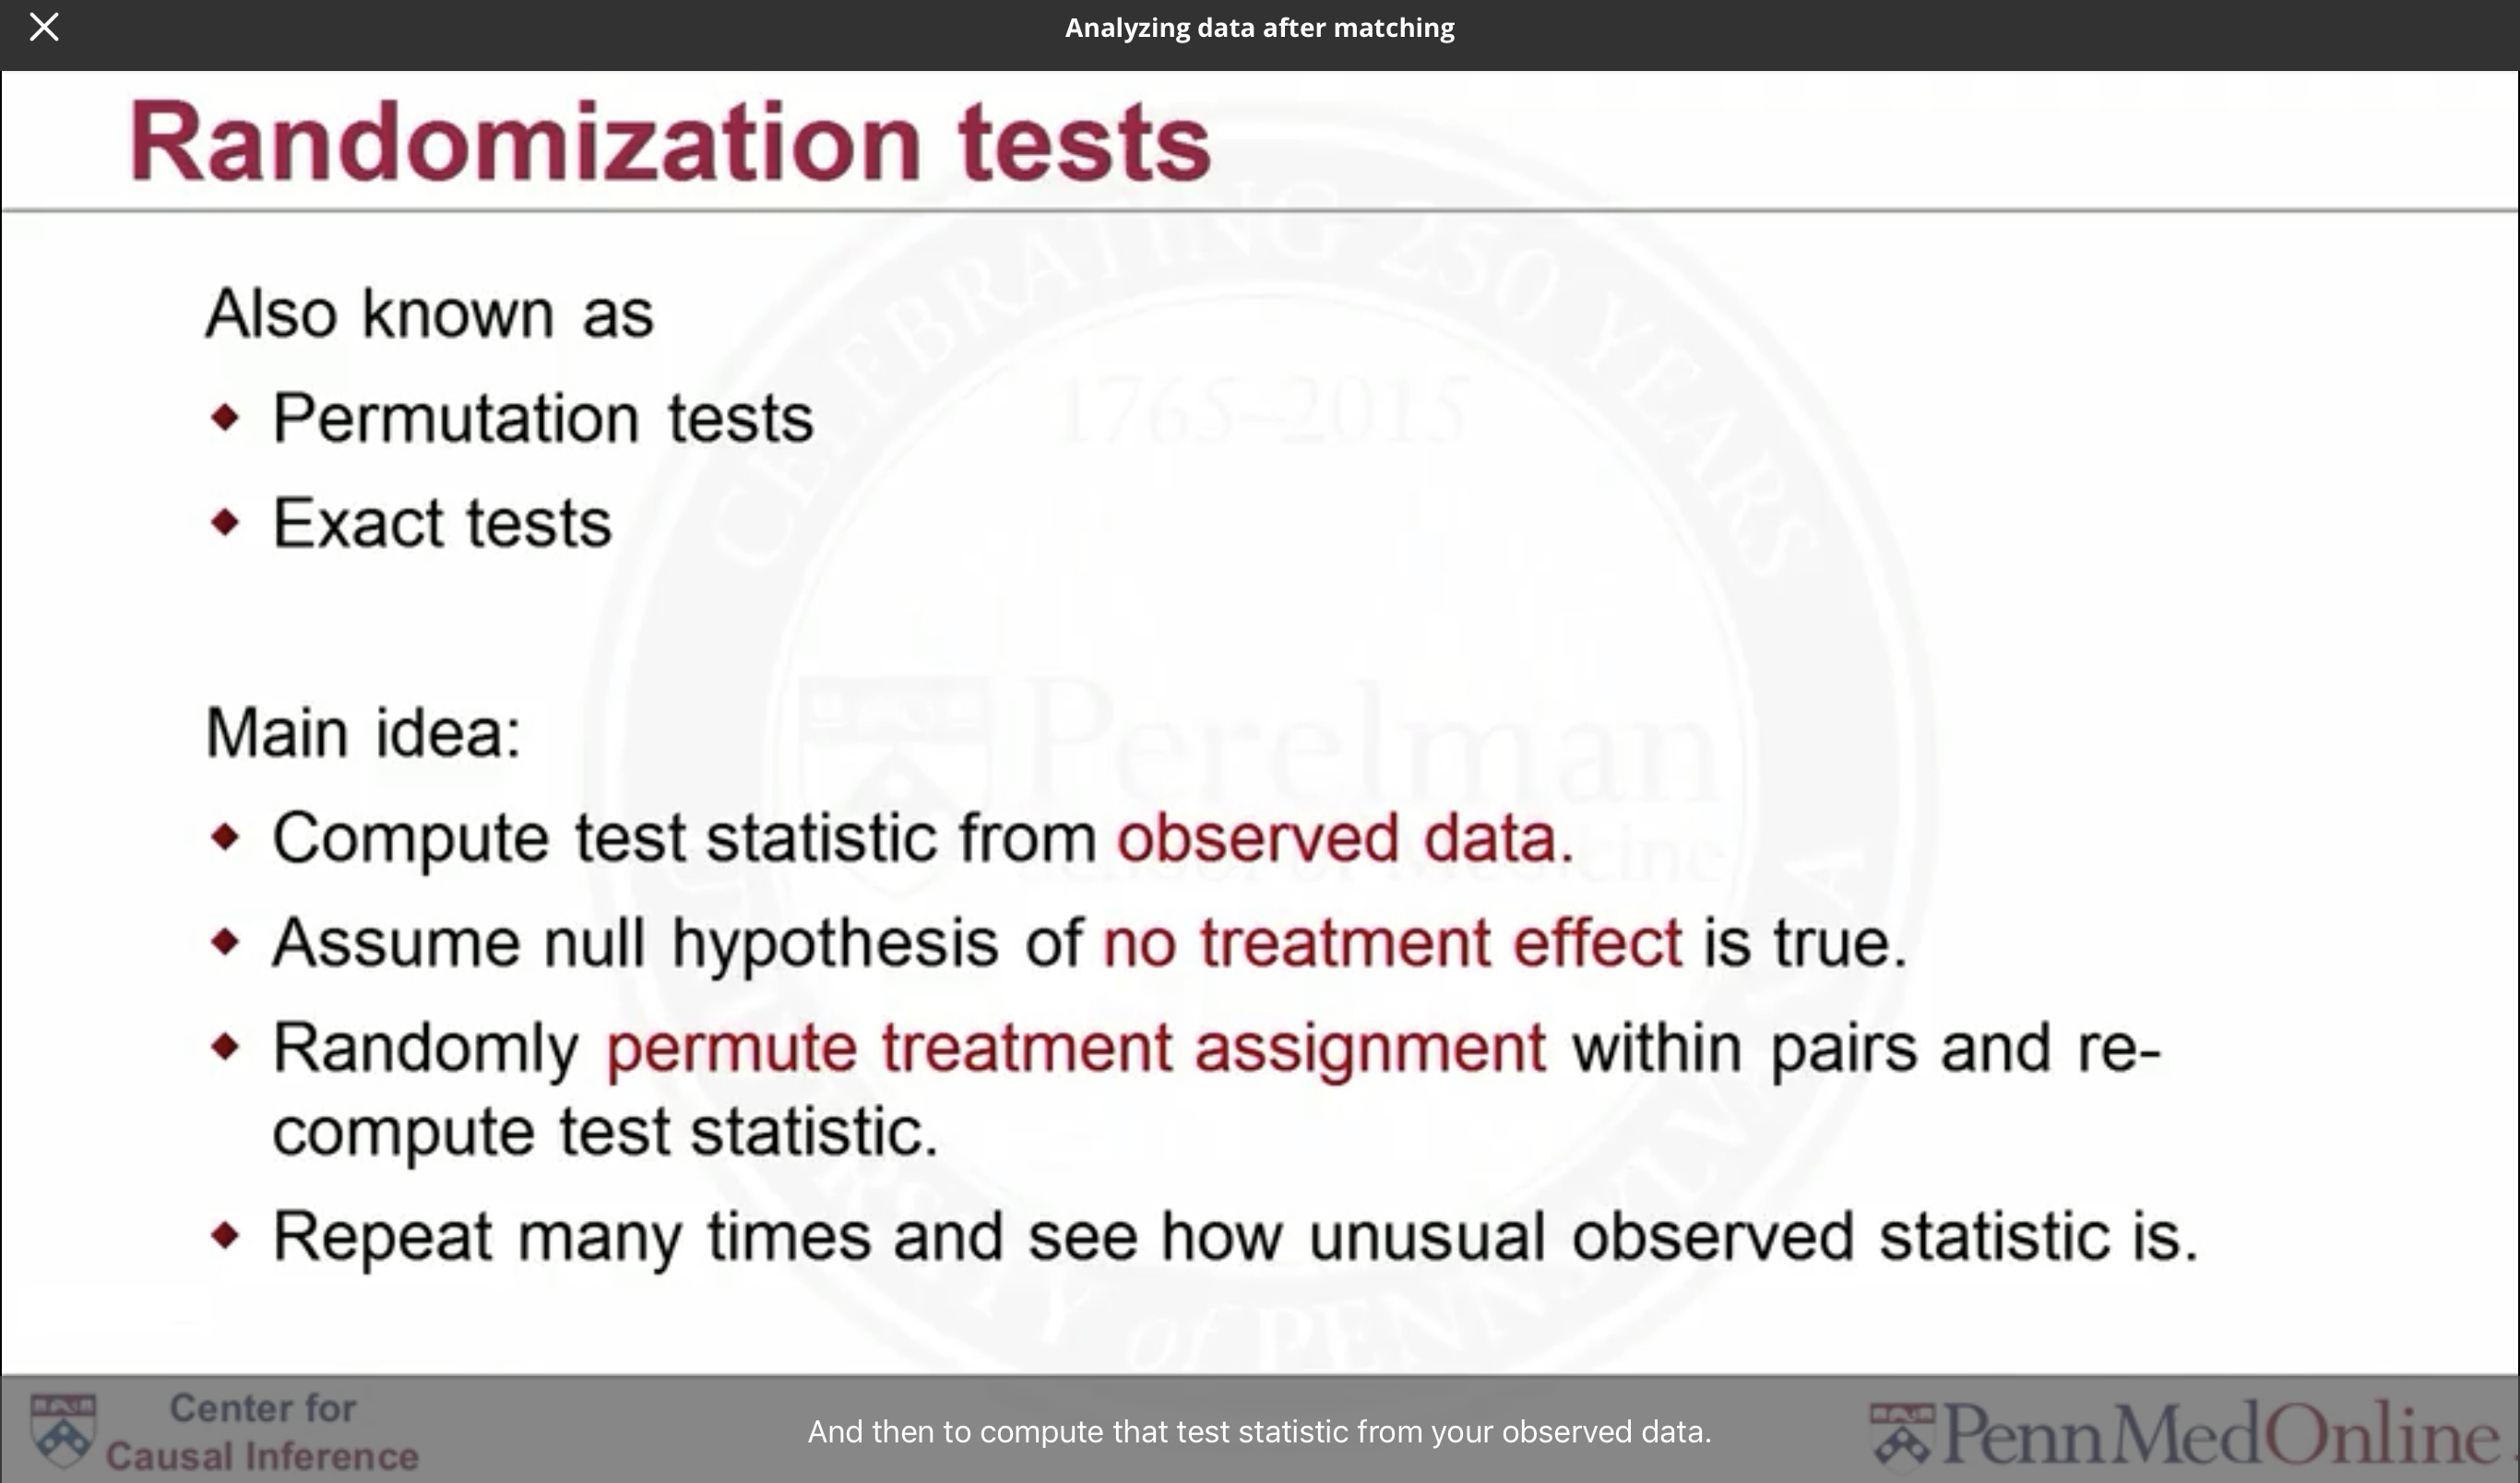
\includegraphics[width=0.8\textwidth]{figure/pertest.jpg}
	\caption{Permutation test}
	\label{pertest}
\end{figure}

Permutation test的思想很简单:构建一个检验统计量,做假设检验. {\bfseries 假设原假设成立},对比original data的test statistic与交换treatment后的permutation data的test statistic是否有明显的差异.
\subsection{Calculation of test statistics}
对于binary outcome,我们可以简单把test statistic取为treated组outcome=1的计数,如Fig.\ref{exper}.
\begin{figure}
	\setlength{\abovecaptionskip}{0pt}     %调整图片标题与图距离
	\setlength{\belowcaptionskip}{10pt}
	\vspace{-0cm}  %调整图片与上文的垂直距离
	\setlength{\abovecaptionskip}{-0cm}   %调整图片标题与图距离
	\setlength{\belowcaptionskip}{-0cm}   %调整图片标题与下文距离
	\centering
	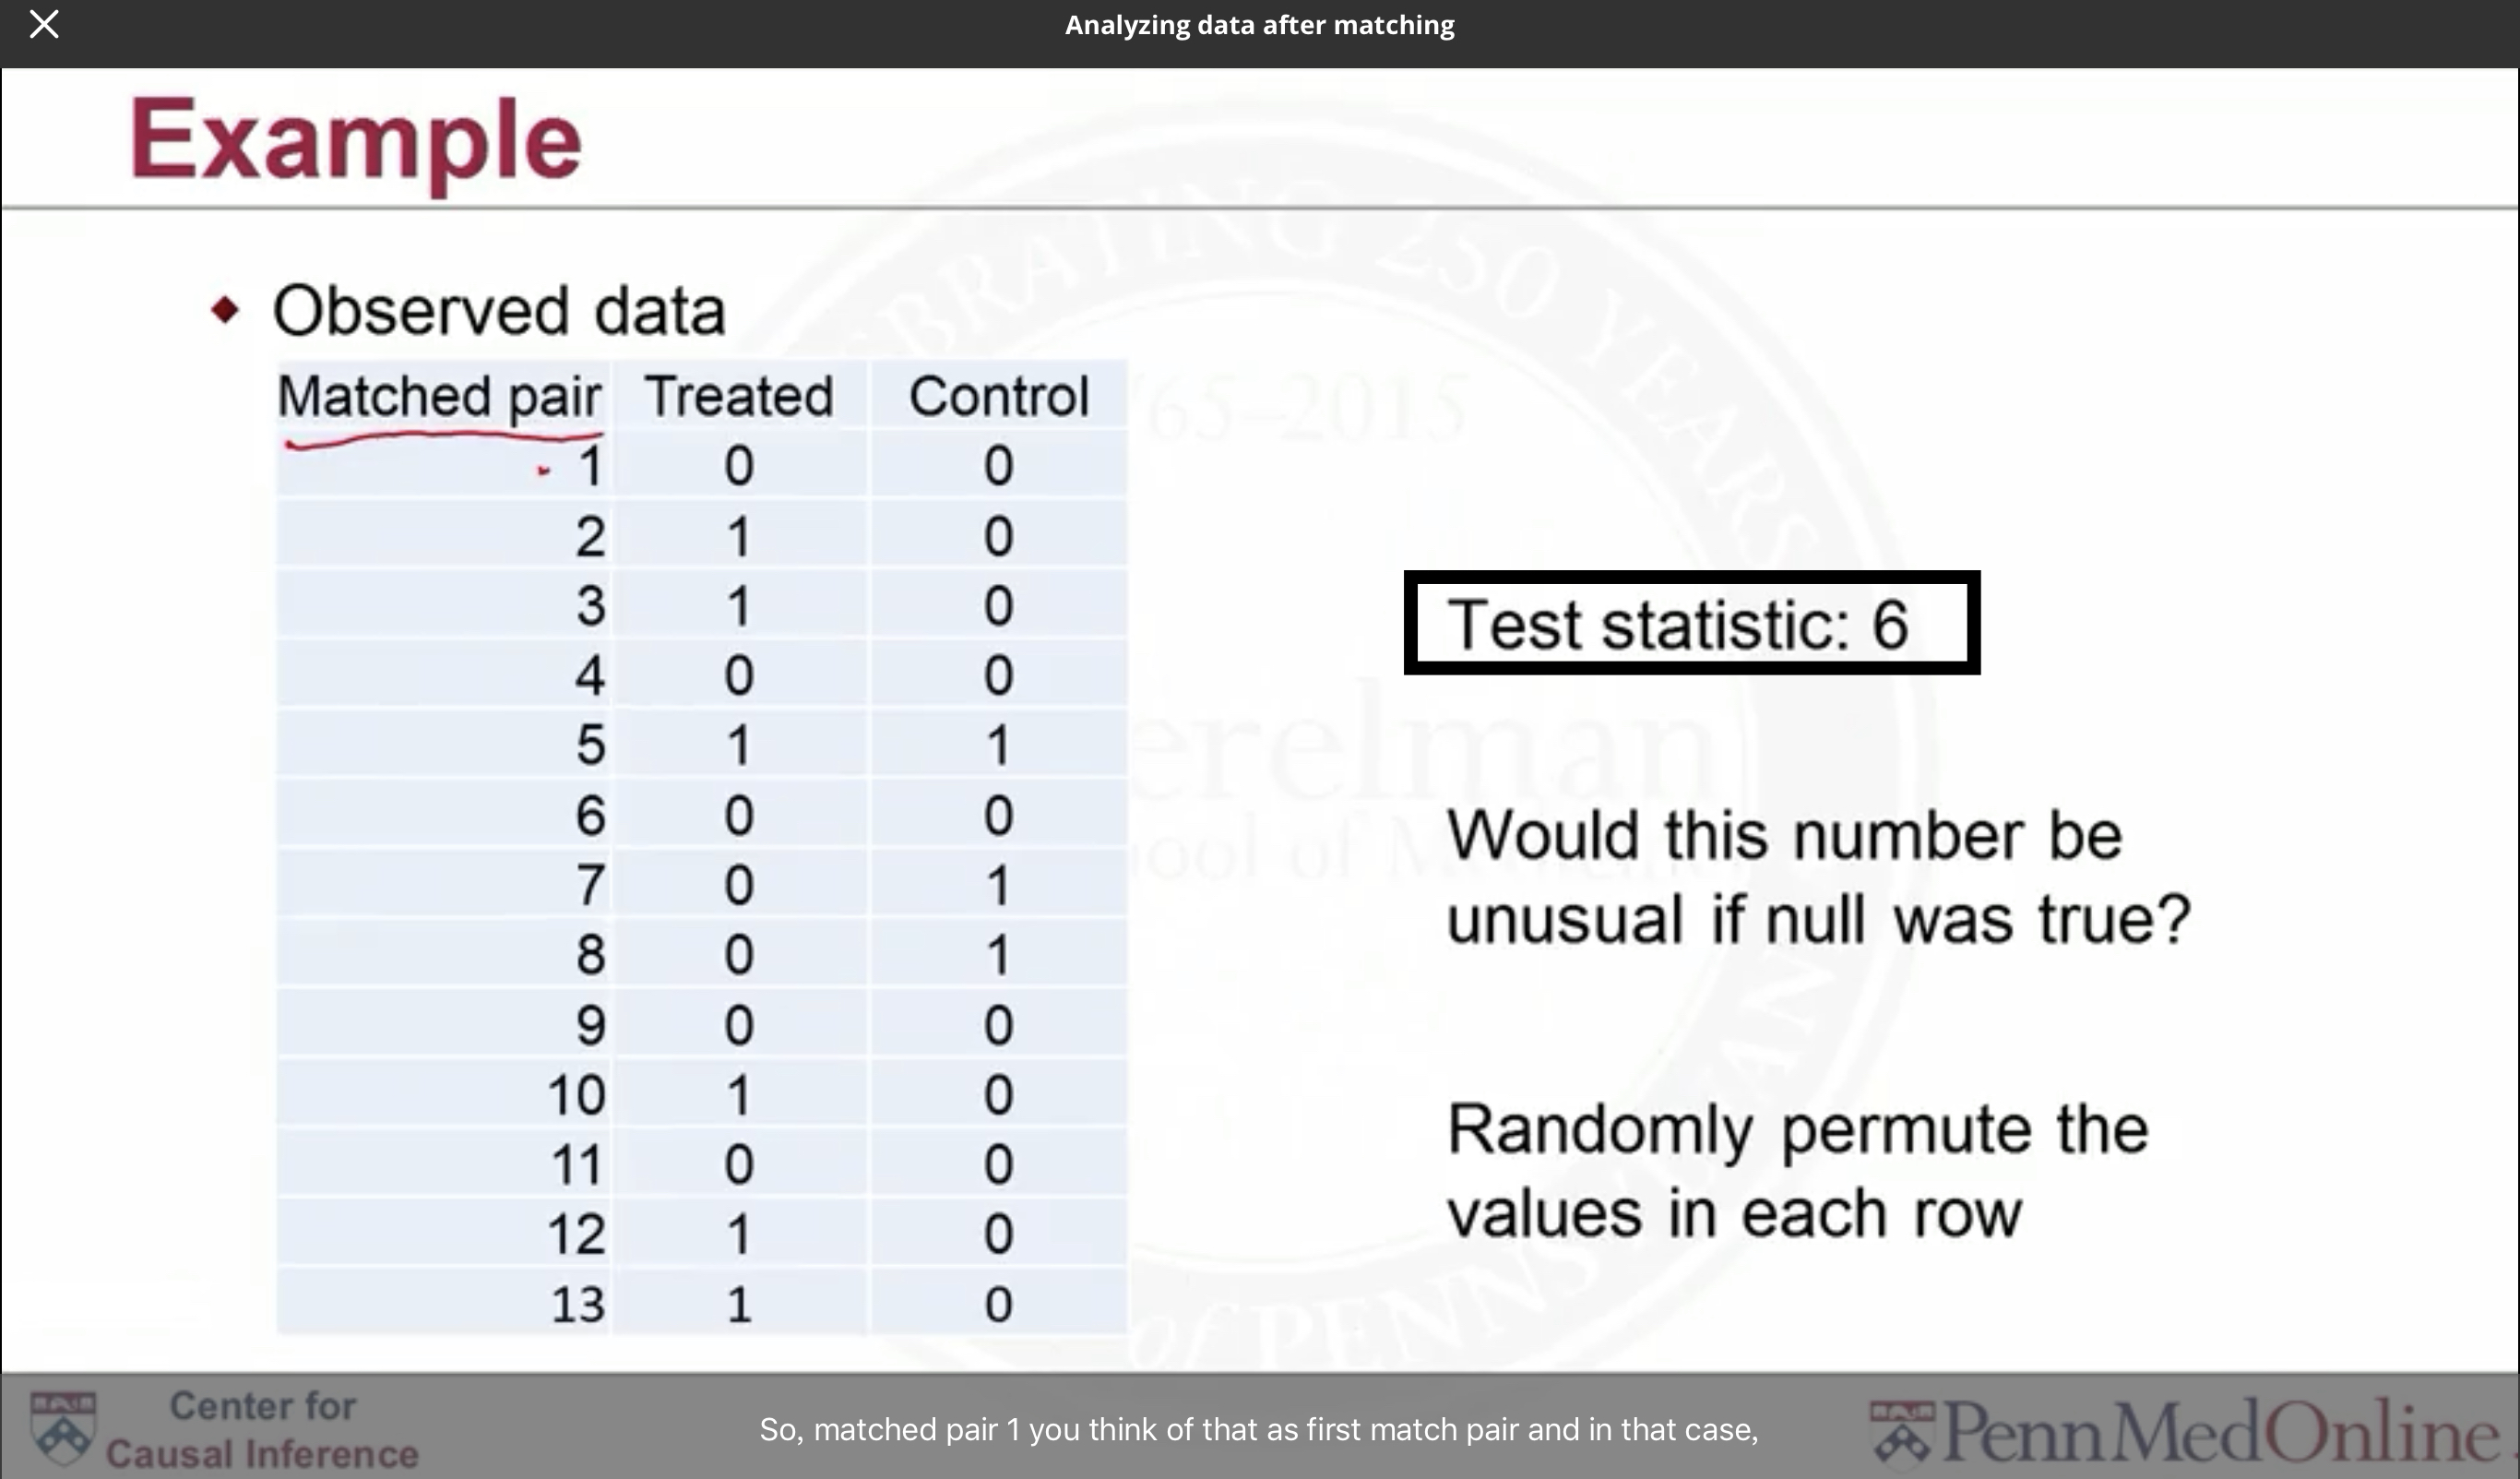
\includegraphics[width=0.8\textwidth]{figure/exper.jpg}
	\caption{Calculation of test statistics}
	\label{exper}
\end{figure}

当然,只进行一次或几次Permutation change可能有偶然性,所以交换treatment的操作可以循环重复K次,然后绘制出test statistics的分布直方图,看统计量集中在哪里. 找出observed data的test statistic,看其是否出现在直方图的集中位置. 

\subsection{Calculation of p value}
或者可以通过计算p值来决定是否接受原假设. p值代表的是在原假设成立的情况下大于观察值或比观察值更极端情况出现的概率. 以Fig.\ref{histts}为例,p值就是将observed data value大于等于6(6,7,8),以及极端值1,2,3出现的概率相加:
\begin{figure}[htbp]
	\setlength{\abovecaptionskip}{0pt}     %调整图片标题与图距离
	\setlength{\belowcaptionskip}{10pt}
	\vspace{-0cm}  %调整图片与上文的垂直距离
	\setlength{\abovecaptionskip}{-0cm}   %调整图片标题与图距离
	\setlength{\belowcaptionskip}{-0cm}   %调整图片标题与下文距离
	\centering
	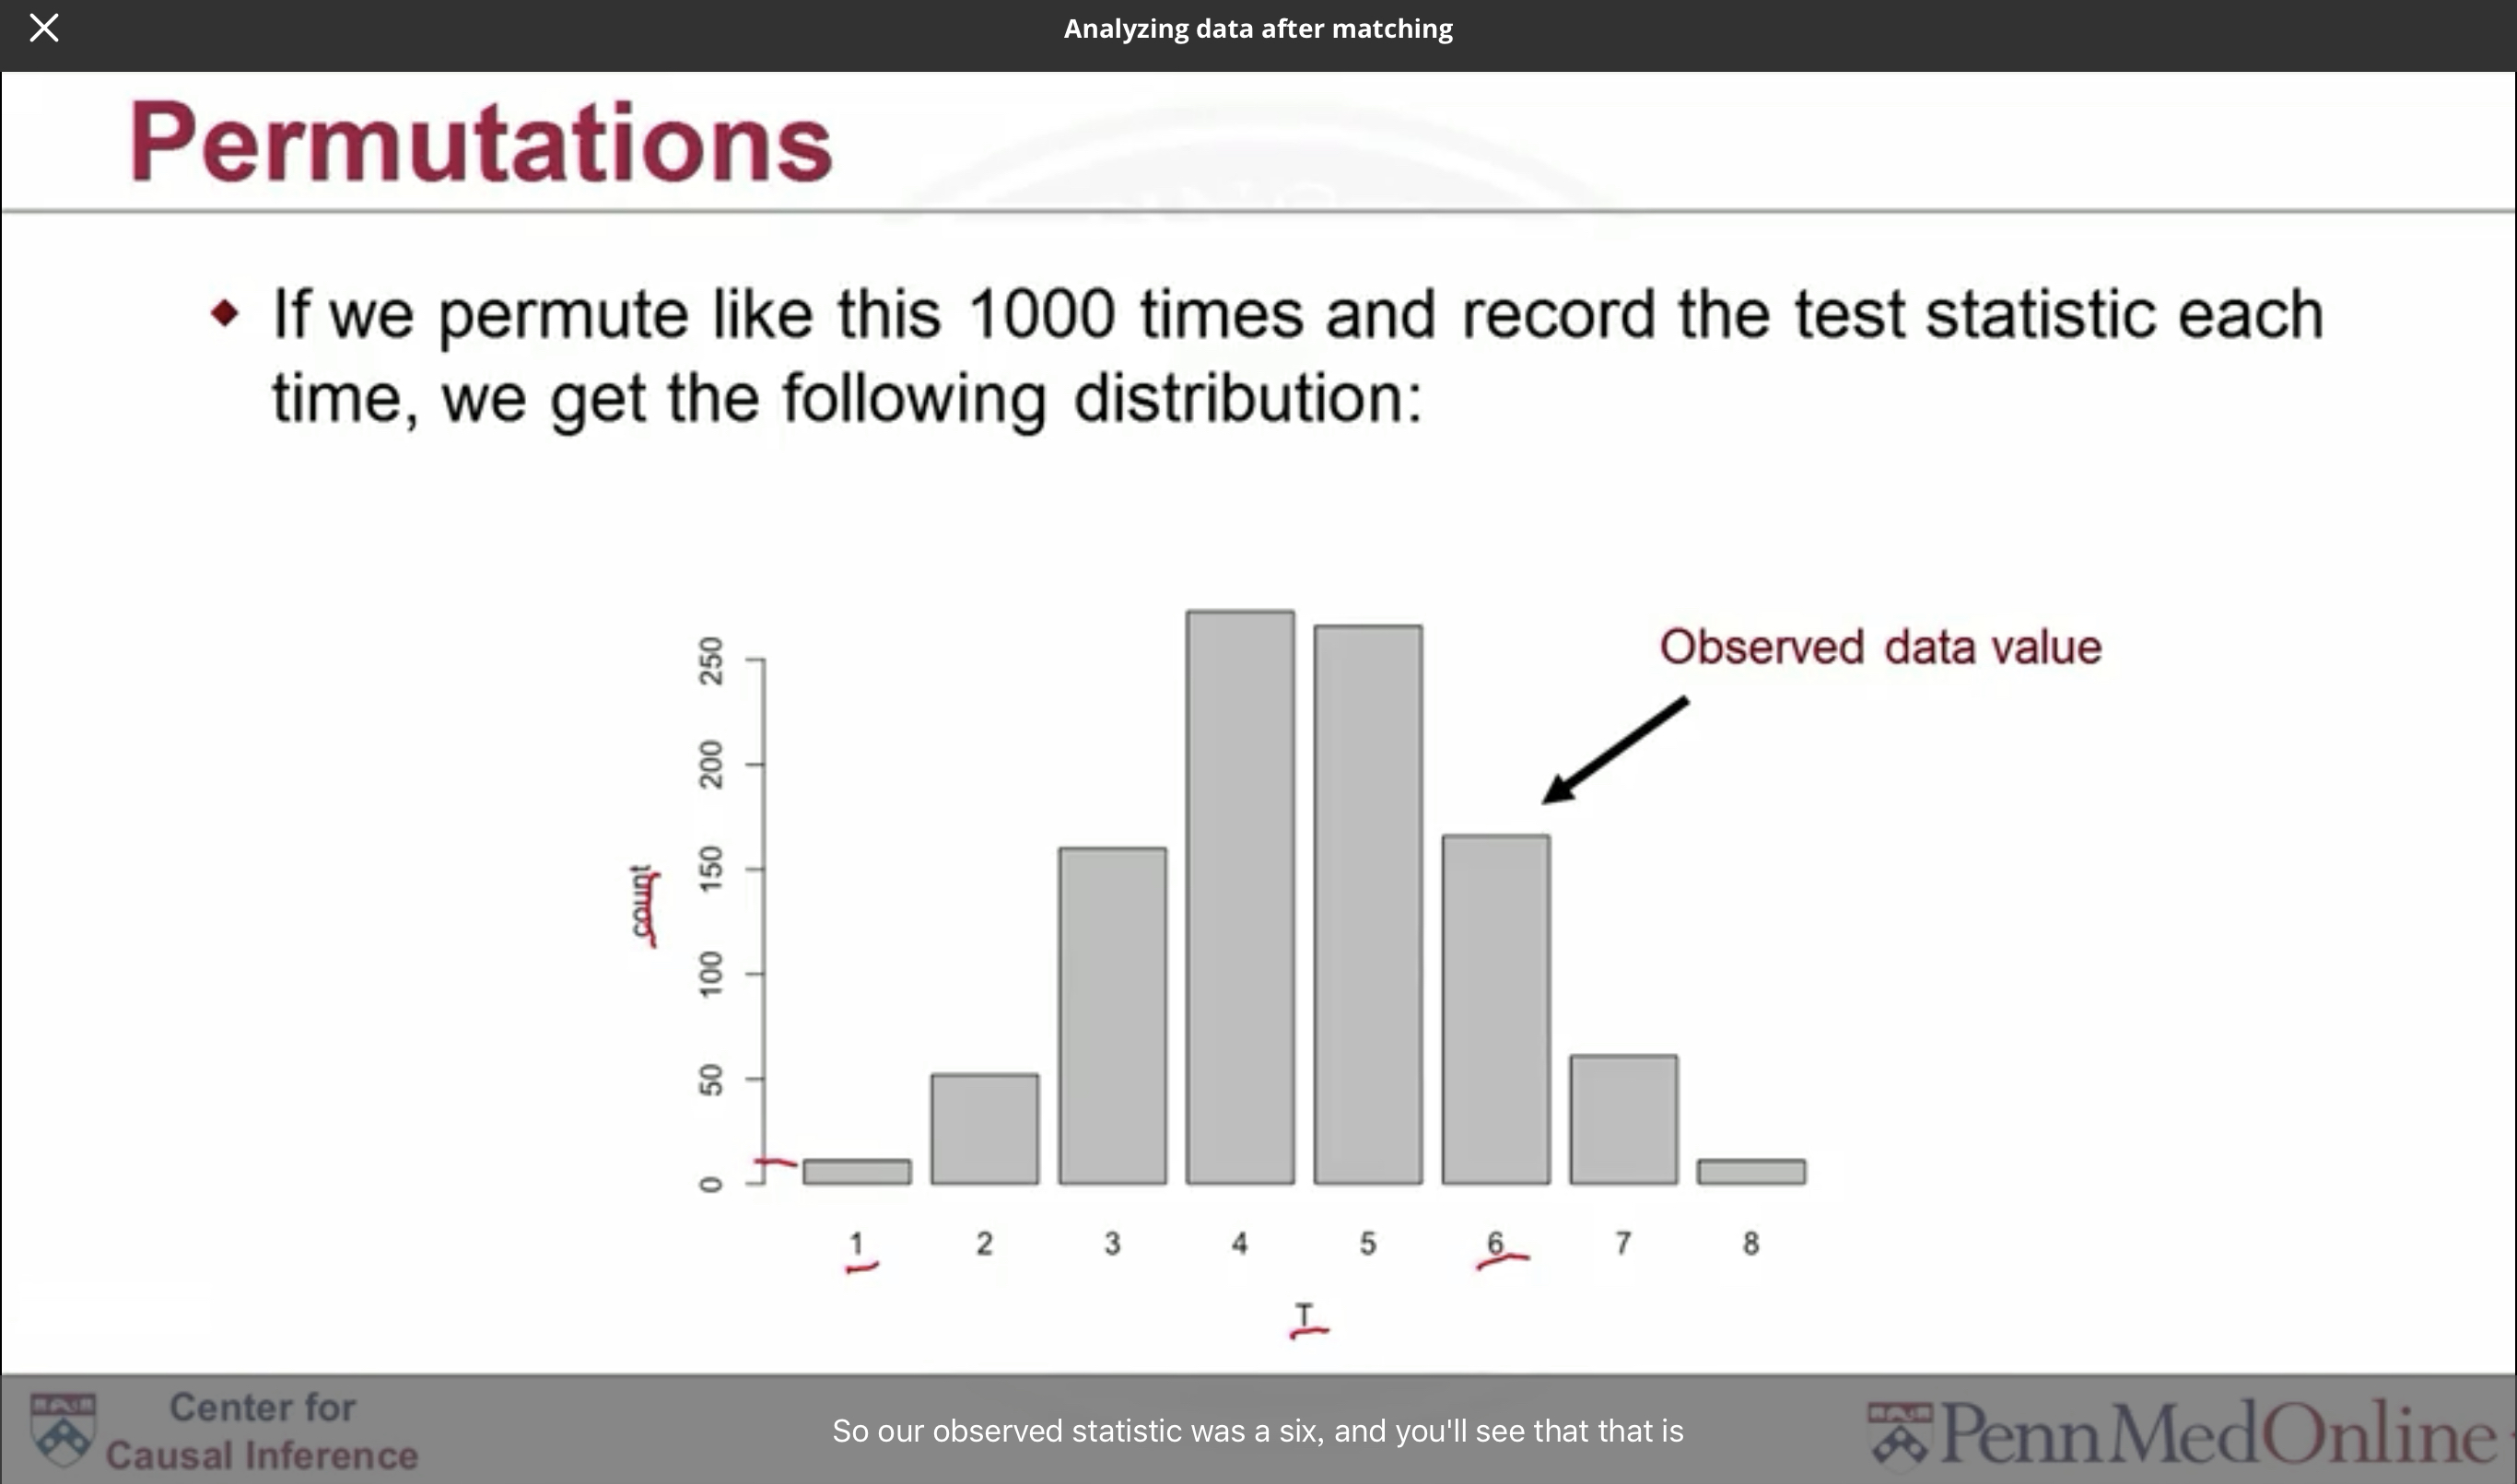
\includegraphics[width=0.8\textwidth]{figure/histts.jpg}
	\caption{Histogram test statistics}
	\label{histts}
\end{figure}

\subsection{Discordant pair}
对于binary outcome来说,交换treated与control只对不一致的pair起作用,对于相同outcome的pair,交换也不会带来什么改变. 

\subsection{McNemar test}
画一个格子点表格,分别计数"Count(outcome=1$|$A=1)","Count(outcome=1$|$A=0)","Count(outcome=0$|$A=1)","Count(outcome=0$|$A=0)". 然后在R中进行mcmemar.test.

\begin{figure}[htbp]
	\setlength{\abovecaptionskip}{0pt}     %调整图片标题与图距离
	\setlength{\belowcaptionskip}{10pt}
	\vspace{-0cm}  %调整图片与上文的垂直距离
	\setlength{\abovecaptionskip}{-0cm}   %调整图片标题与图距离
	\setlength{\belowcaptionskip}{-0cm}   %调整图片标题与下文距离
	\centering
	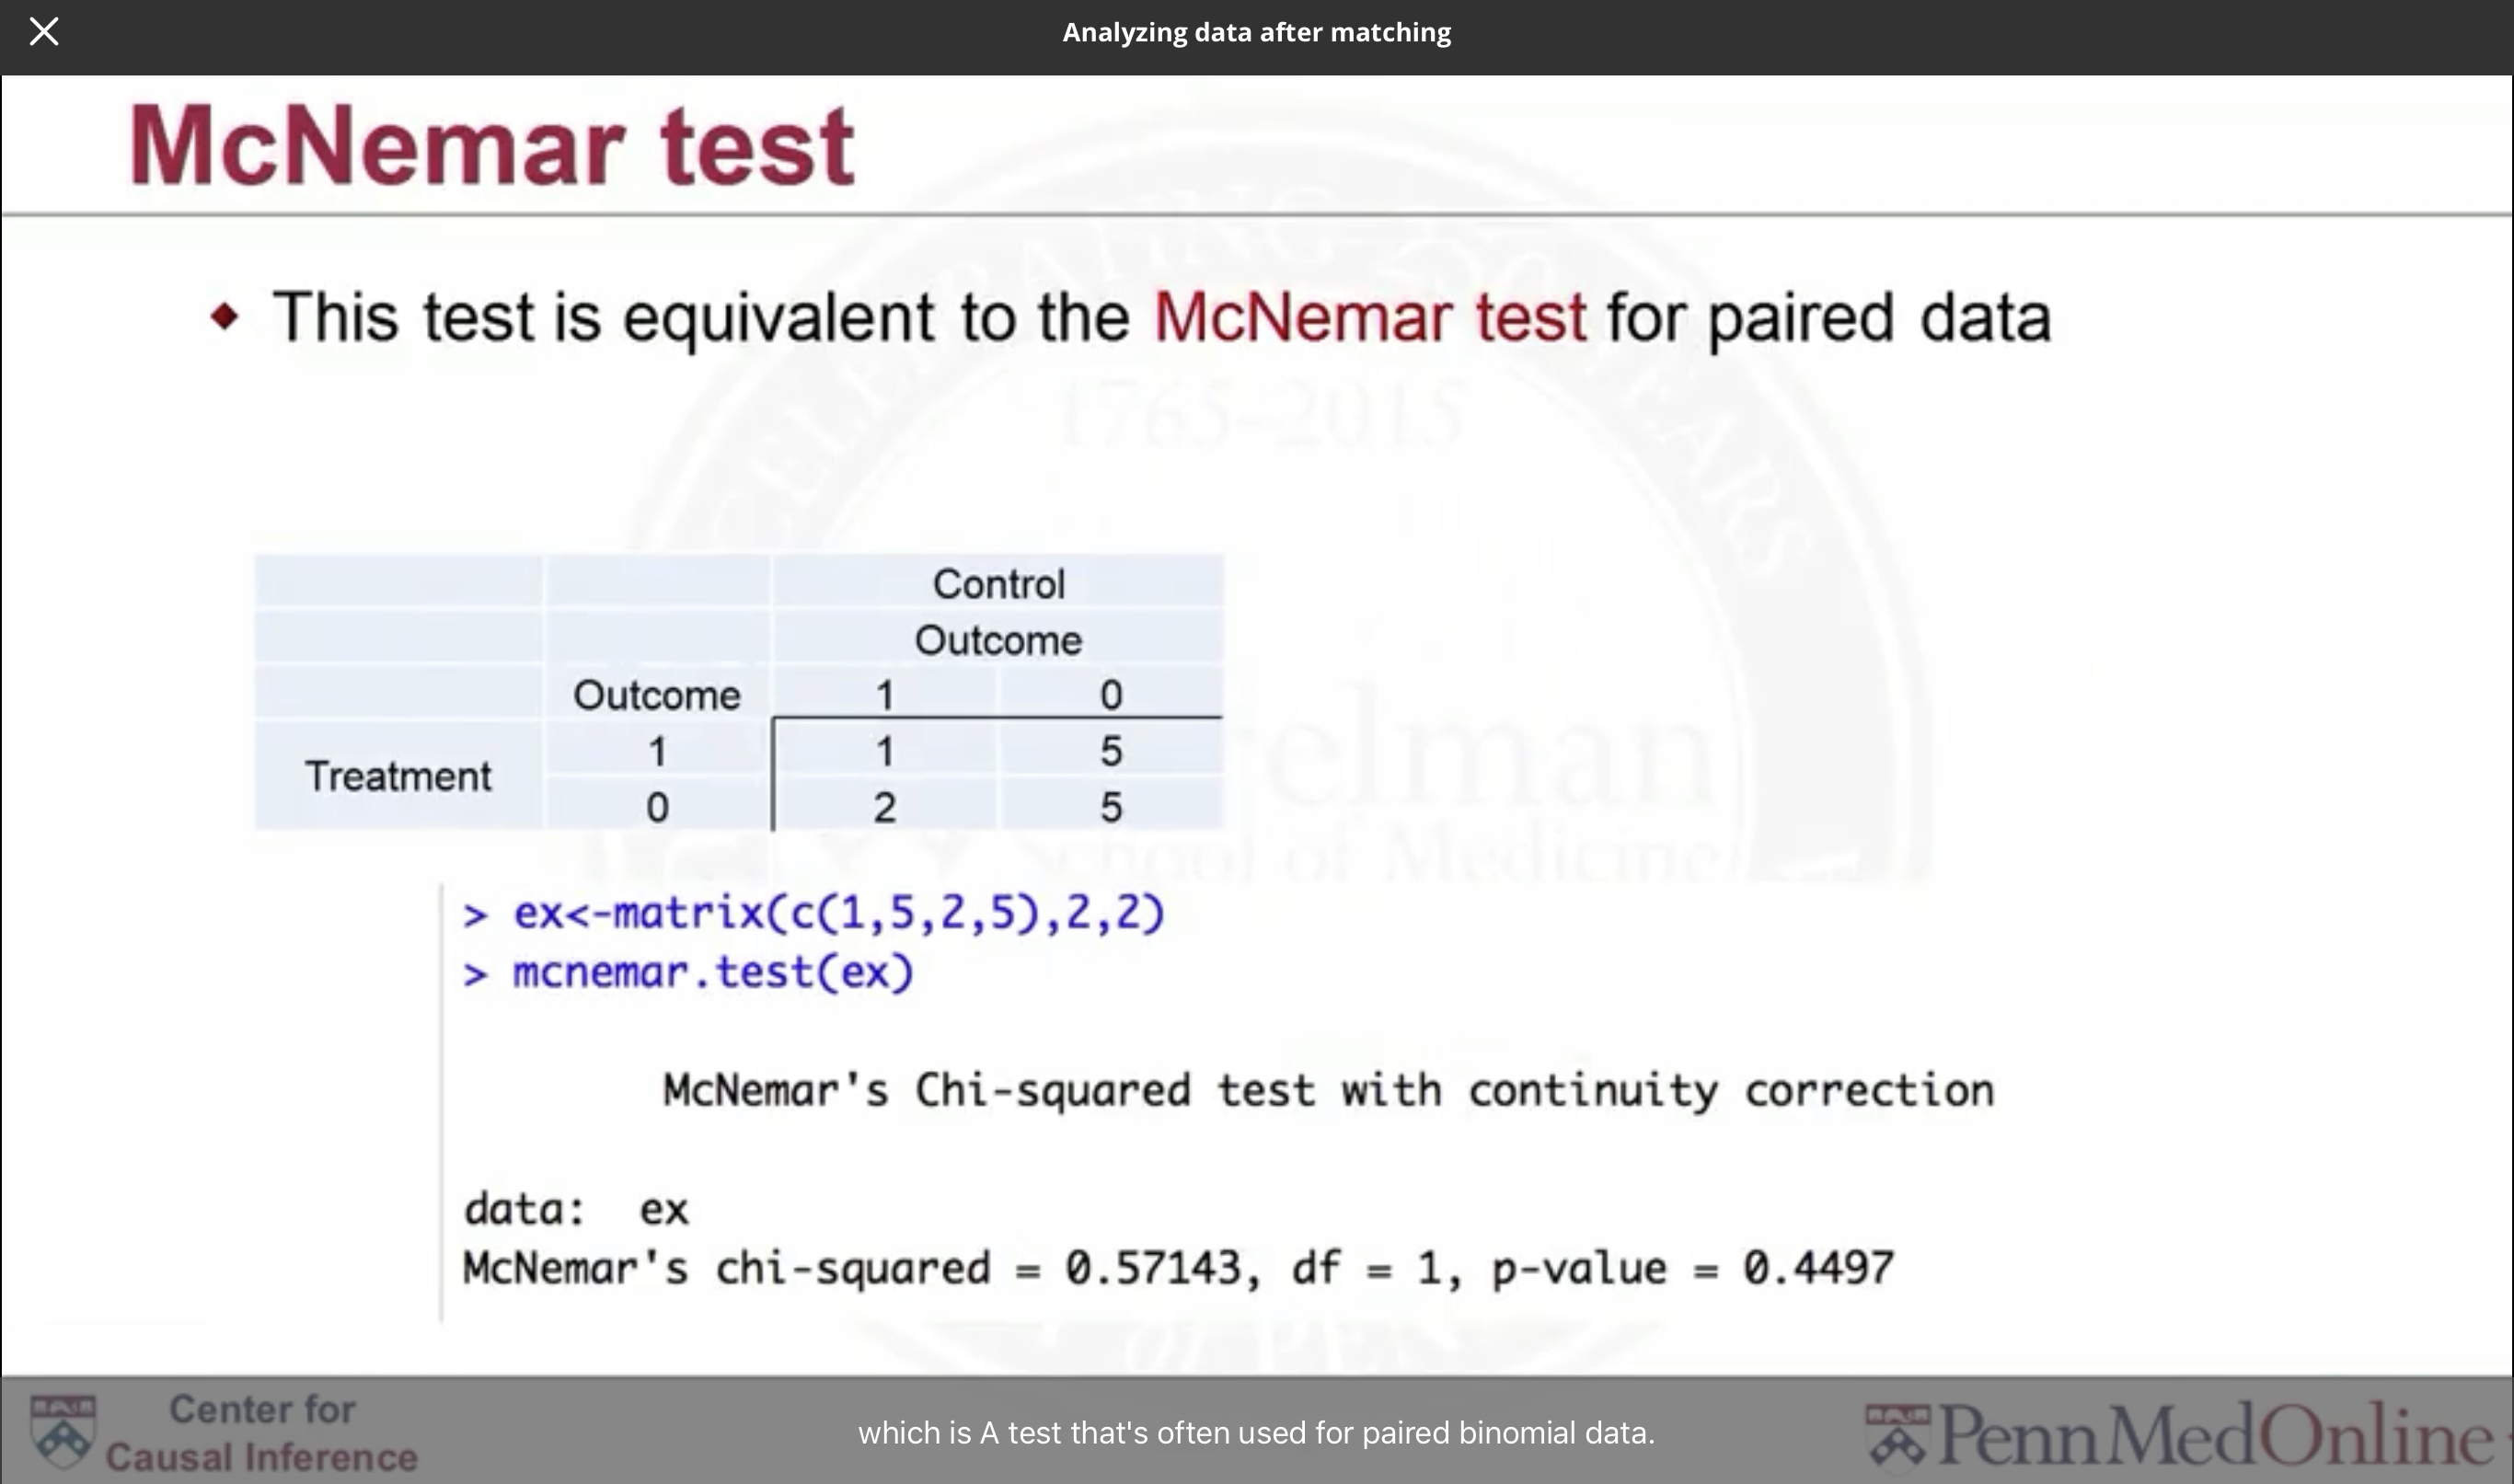
\includegraphics[width=0.8 \textwidth]{figure/mcnemar.jpg}
	\caption{McNemar test}
	\label{mcnemar}
\end{figure}

\section{Sensitivity analysis}
\section{Propensity score}
\section{Propensity score matching}
\section{Data Example: Propensity score match i R}

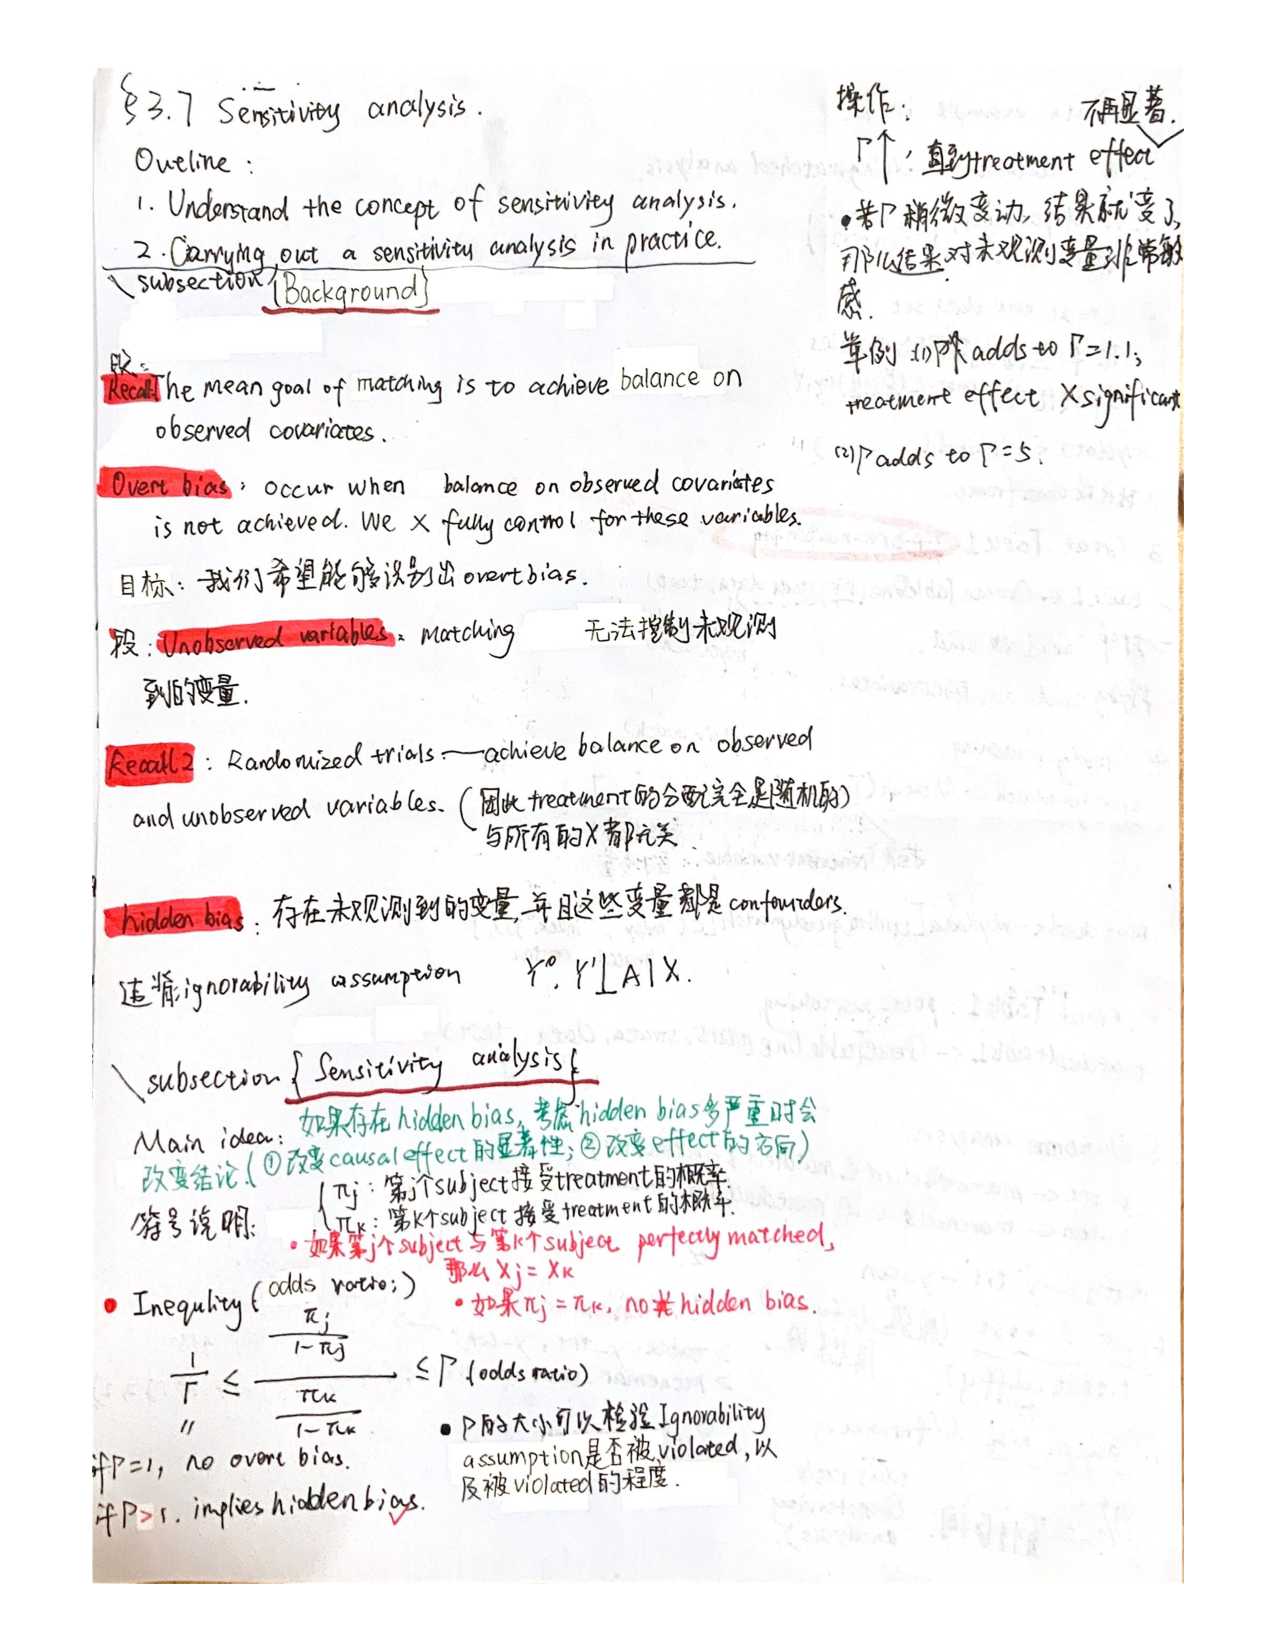
\includepdf[pages=-]{figure/sen.pdf}
\begin{figure}[htbp]
	\setlength{\abovecaptionskip}{0pt}     %调整图片标题与图距离
	\setlength{\belowcaptionskip}{10pt}
	\vspace{-0cm}  %调整图片与上文的垂直距离
	\setlength{\abovecaptionskip}{-0cm}   %调整图片标题与图距离
	\setlength{\belowcaptionskip}{-0cm}   %调整图片标题与下文距离
	\centering
	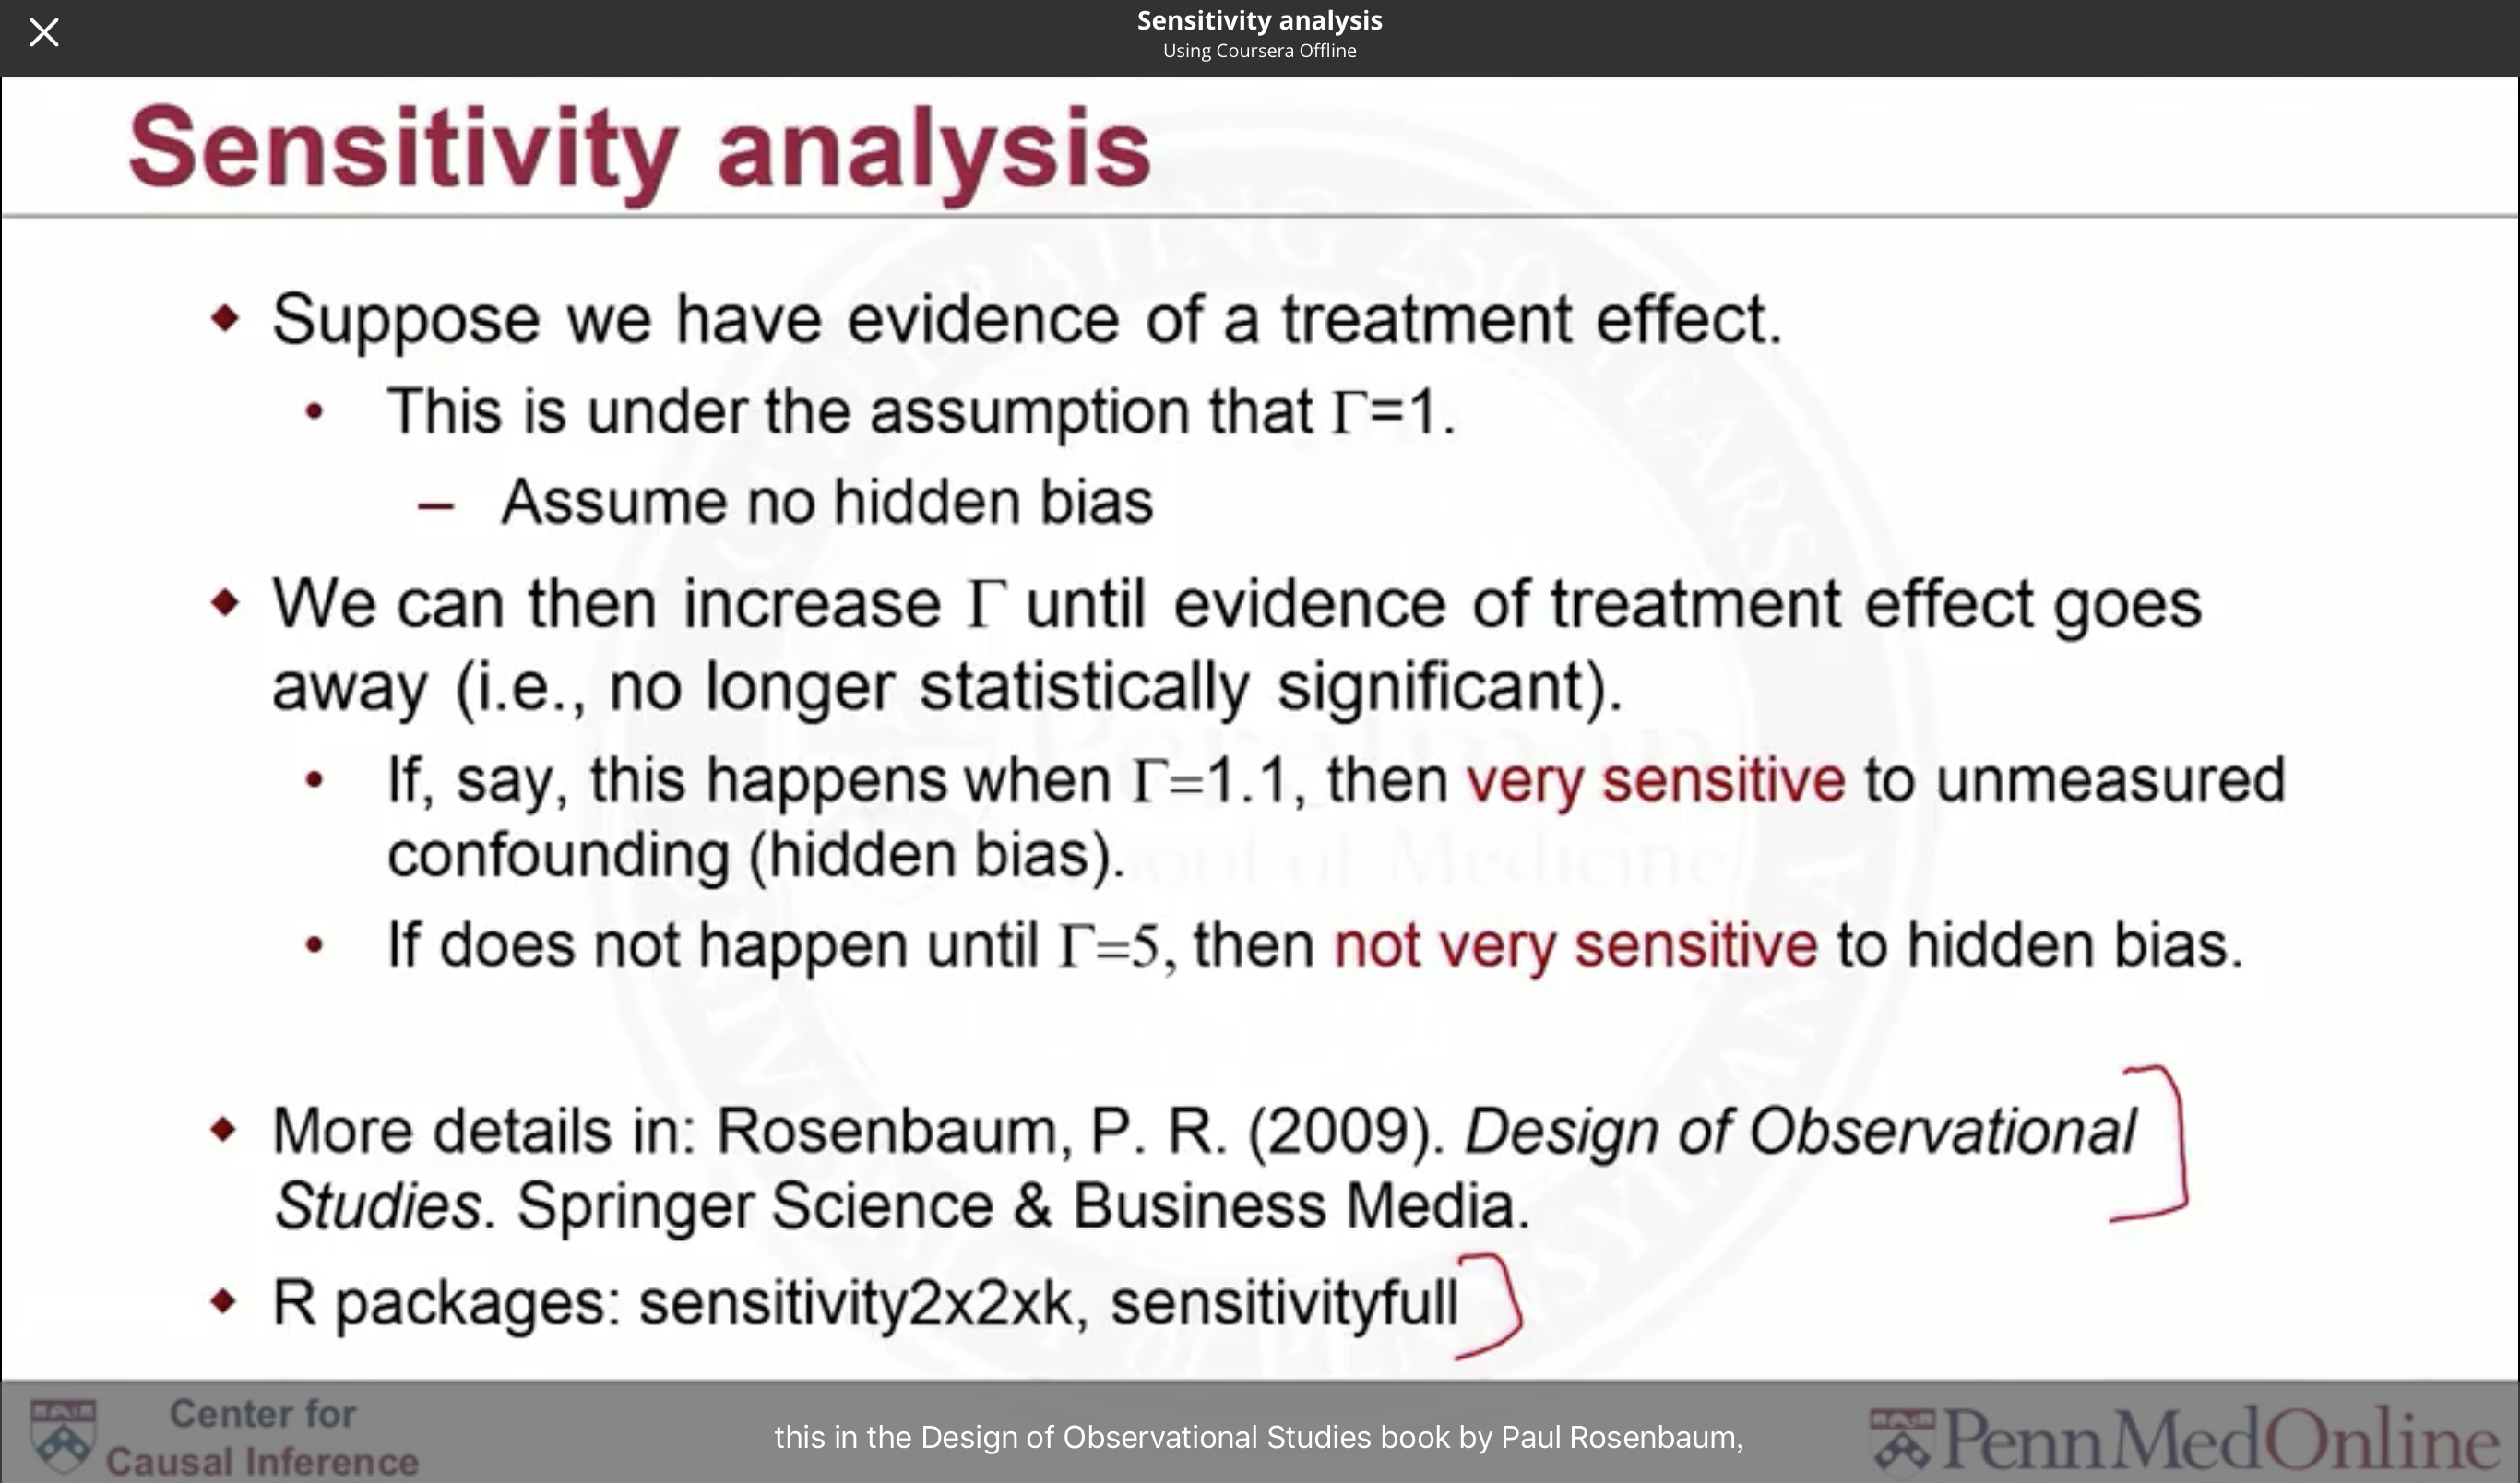
\includegraphics[width=0.8\textwidth]{figure/sensitivity.jpg}
	\caption{Sensitivity analysis}
	\label{sen}
\end{figure}

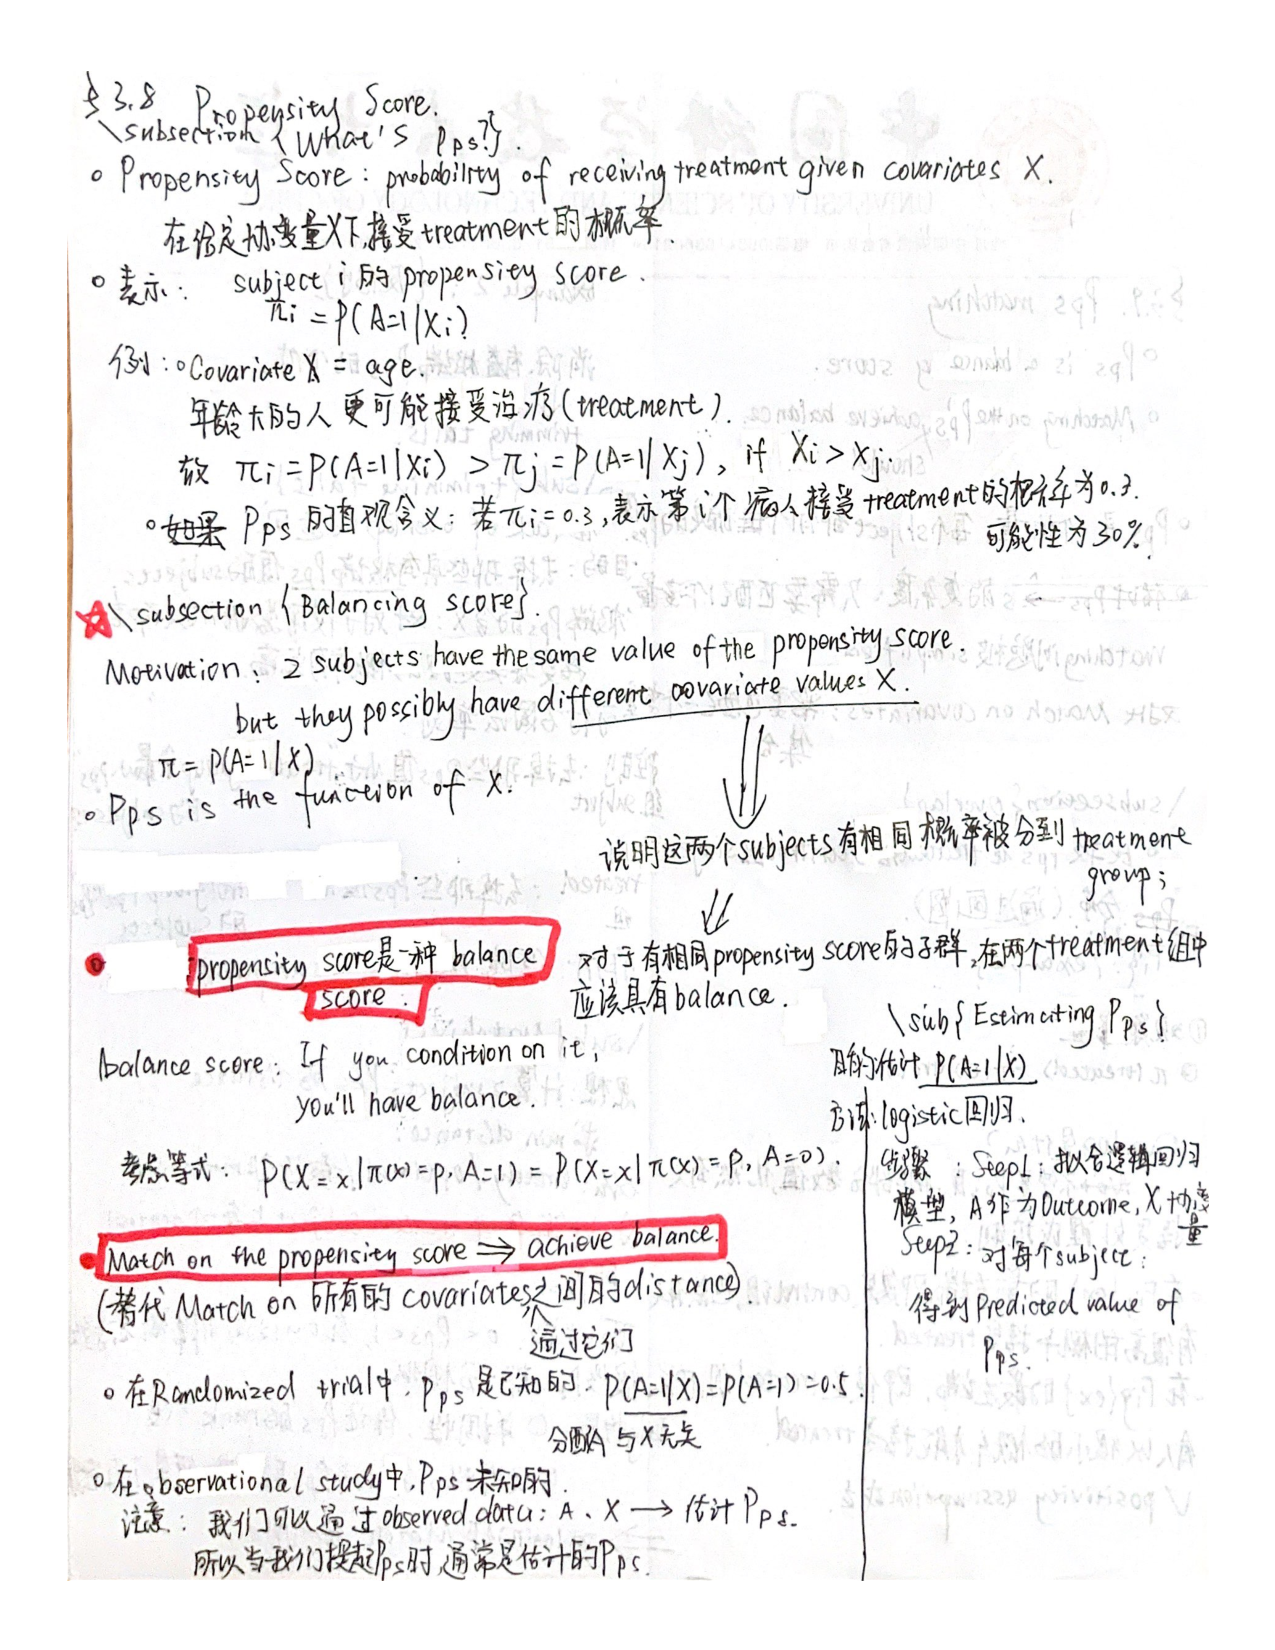
\includepdf[pages={1}]{figure/3pdf.pdf}
\includepdf[pages={2,3}]{figure/3pdf.pdf}

\begin{figure}[htbp]
	\setlength{\abovecaptionskip}{0pt}     %调整图片标题与图距离
	\setlength{\belowcaptionskip}{10pt}
	\vspace{-0cm}  %调整图片与上文的垂直距离
	\setlength{\abovecaptionskip}{-0cm}   %调整图片标题与图距离
	\setlength{\belowcaptionskip}{-0cm}   %调整图片标题与下文距离
	\centering
	\includegraphics[width=0.8\textwidth]{figure/Example.jpg}
	\caption{Example}
	\label{Example}
\end{figure}
\begin{figure}[htbp]
	\setlength{\abovecaptionskip}{0pt}     %调整图片标题与图距离
	\setlength{\belowcaptionskip}{10pt}
	\vspace{-0cm}  %调整图片与上文的垂直距离
	\setlength{\abovecaptionskip}{-0cm}   %调整图片标题与图距离
	\setlength{\belowcaptionskip}{-0cm}   %调整图片标题与下文距离
	\centering
	\includegraphics[width=0.8\textwidth]{figure/Example2.jpg}
	\caption{Example2}
	\label{Example2}
\end{figure}

\begin{figure}[htbp]
	\setlength{\abovecaptionskip}{0pt}     %调整图片标题与图距离
	\setlength{\belowcaptionskip}{10pt}
	\vspace{-0cm}  %调整图片与上文的垂直距离
	\setlength{\abovecaptionskip}{-0cm}   %调整图片标题与图距离
	\setlength{\belowcaptionskip}{-0cm}   %调整图片标题与下文距离
	\centering
	\includegraphics[width=0.8\textwidth]{figure/trim.jpg}
	\caption{Trimming tails}
	\label{trim}
\end{figure}

\begin{figure}[htbp]
	\setlength{\abovecaptionskip}{0pt}     %调整图片标题与图距离
	\setlength{\belowcaptionskip}{10pt}
	\vspace{-0cm}  %调整图片与上文的垂直距离
	\setlength{\abovecaptionskip}{-0cm}   %调整图片标题与图距离
	\setlength{\belowcaptionskip}{-0cm}   %调整图片标题与下文距离
	\centering
	\includegraphics[width=0.8\textwidth]{figure/caliper.jpg}
	\caption{Caliper}
	\label{caliper}
\end{figure}


\includepdf[pages=-]{figure/psmatchinR.pdf}
    \chapter{Inverse Probability of Treatemnt Weighting}
本章笔记均为书面形式,只汇总概要,具体内容看书面笔记.

\section{Intuition for IPTW}
\subsection{IPTW的计算方法}
\subsection{IPTW的作用}
\begin{itemize}
	\item \r{IPTW的作用:}对每一种X的取值(在Propensity score相同的subjects中),令treated subjects的counting和control subjects的counting相等.
\end{itemize}
	
	
\section{More intuition for IPTW}
这一节课的重点在于理解Pseudo-population的含义、作用,以及如何构建pseudo-population.

\r{Goal:} Using weihgting to create a pseudo-population where there is no confounding.

\section{Marginal structual model}
\subsection{Introduction to MSMs}
\r{MSM is a model for the mean of potential outcomes for whole population.}
\begin{itemize}
	\item Marginal:Model does not conditional on confounders(X). 也就是说模型不以X的某个取值为条件(E(Y$|$X=x)),而是遍历X的全部取值,是一种边缘(marginal)模型.
	\item Structural: 模型是针对potential outcomes建立的(E($Y^1$),E($Y^0$)),而不是Observed outcomes. 
	\item 模型针对的是whole population,而不是subpopulation.
\end{itemize}

\subsection{Linear MSM}
\subsection{Logistic MSM for binary outcome}
\subsection{MSM with effect modification}
\begin{itemize}
	\item Model includes effect modifiers V. V is a variable that modifies the effect of A. For example, V could be \r{diabetes, sex, race,...}, these variables could change the effect of treatment. \g{That means in different value of V, causal effect are different.}
\end{itemize}

\subsection{General MSM}
\subsection{Key issue of MSM}
建立MSM的难点在于模型是针对potential outcomes建立的,然而实际上我们只能获取observed outcome,如何在值给定observed outcome的情况下估计模型的参数?


\section{IPTW estimaion}
这一节主要讲述如何估计Marginal structual model中的参数.
\subsection{Recall: Estimation in linear regression model}
\subsection{Difference between MSM and regression model}

\begin{itemize}
	\item 若建立regression model来估计A的causal effect,模型为
	\begin{equation}
	g(E(Y|A))=\psi_0+\psi_1 A.
	\end{equation}
	此时我们估计的是$E(Y|A)=g^{-1}(\psi_0+\psi_1 A)$,这里的A是固定的某个取值a,针对的是A=a的subpopulation.
	 
	\item MSM模型为
	\begin{equation}
	g(E(Y^a))=\psi_0+\psi_1 A
	\end{equation}
	此时我们估计的是$E(Y^a)=g^{-1}(\psi_0+\psi_1 A)$,这里的A取值未定,可以是任意的取值.
\end{itemize}

\subsection{Why different?}
MSM与regression model的区别是因为\r{confounding的存在}. 但是,我们注意到在randomized trial中$E(Y|A=a)=E(Y^a)$,也就是说randomized trial中没有confounding影响,可以拟合regression model,模型的参数就是causal effect. 

这给我们提供了一种思路:既然在randomized trial中可以拟合回归模型,那我们可以尽量去构建randomized trial,然后做回归.

\subsection{利用Pesudo-population近似randomized trials}
在4.2节中,我们知道可以使用IPTW的方法构建Pesudo-population.

\begin{itemize}
	\item Pesudo-population is free from confounding.(Under ignorability and positivity assumption)
\end{itemize}

\subsection{Steps in estimating parameters from MSM}

Issue of IPTW: 使用weighting的方法人为地扩大了population siz,使模型的error更大了.

\section{Assessing balance and Distribution of weights}
Task: 检查weighting之后covariate balance是否实现.
Goal: After weighting sample is equal to randomized trial.
\subsection{Standardized difference}
\begin{itemize}
	\item 注意是对weighting后的样本做检验,而不是原样本!
	\item 列出table one.
\end{itemize} 

\section{Distribution of weights}
\begin{itemize}
	\item large weight $\longrightarrow$ large standard error.
\end{itemize}
\subsection{Bootstrapping}
\subsection{Relationship with positivity assumption}
large weight $\longrightarrow$ very small propensity score $\longrightarrow$ very small probability to get treated $\longrightarrow$ violate positivity assumption.


\section{Remedies for large weights}
\subsection{Trimming the tails}
\subsection{Weight trunction}

%\includepdf[pages=-]{figure/4.1.pdf}
%\includepdf[pages=-]{figure/4.3.pdf}
%\includepdf[pages=-]{figure/4.4.pdf}
%\includepdf[pages=-]{figure/4.56.pdf}
%\includepdf[pages=-]{figure/4.7.pdf}
    \chapter{Instrumental variabels methods}
本章笔记均为书面形式,只汇总概要,具体内容看书面笔记.

这一章主要讲述了一种估计causal effect的新思路. 

在第三章和第四章中,估计causal effect的重要假设就是ignorability assumption,给定covariates X,treatment与potential outcome独立. 控制这些covariates足够控制所有的confounding.

然而当存在unmeasured confounding时, match和iptw的方法得到的估计量是有偏差的,这种偏差称为hidden bias,是一种潜在的偏差. 本章讲述的instrumental variable methods可以在存在unmeasured confounding的情况下,很好地解决causal effect的估计问题. 只不过此时我们不再是估计average causal effect,而是local average causal effect,针对的估计对象从whole population变成了subpopulation(Compliers).

\section{Introduction to instrumental variables}
\subsection{Two types of causal graphics}
\subsection{The meaning and characters of Z}


\section{Randomized trials with noncompliance}
\subsection{Regard Z as treatment assignment}
\begin{itemize}
	\item The difference between assigned treatment and treatment received.
\end{itemize}
\subsection{Noncompliance}
\subsection{Potential treatment}
\subsection{Causal effect of Z on A}
\subsection{Causal effect of Z on Y}
\subsection{Causal effect of A on Y}


\section{Compliance classes}
\subsection{Four classes of subpopulation}
\begin{itemize}
	\item Principle stratification according to potential treatment$A^0,A^1$.
\end{itemize}

\subsection{Local average treatment effect}
\begin{itemize}
	\item Population causal effect and local causal effect.
\end{itemize}

\subsection{Four classes in Observational data}

\section{Assumptions}
\subsection{Assumptions about IVs}
\subsection{Assumptions about identification of causal effect}

\section{Causal effect identification and estimation}
\begin{itemize}
	\item Intention to treat effect(ITT).  We can identify ITT. 因为Z是randomized的,所以potential outcome的分布与Y的条件分布存在一一对应关系. 
	\begin{equation}
	ITT=E(Y^{Z=1}-Y^{Z=0})=E(Y|Z=1)-E(Y|Z=0).
	\end{equation} 
	\item 注意如何从ITT推导出Complier average causal effect.
	\item Compliers所占的比重推导. P(Compliers)=E(A$|$Z=1)-E(A$|$Z=0).
	\item CACT $>=$ ITT. 分析原因.
\end{itemize}

\section{IVs in observational data}
\subsection{Identifying an IV}
使用IV的挑战在于:如何寻找一个有效的工具变量,使之只影响treatment,而不影响outcome.

在这一节中举例说明了什么样的变量可以作为工具变量,并给出了三个常用的工具变量实例:
\begin{itemize}
	\item Mendelian randomization assumption: genetic variant.
	\item Provider preference(分配treatment的人的偏好).
	\item Quarter of birth.
\end{itemize}

\section{Two-stage regression}
\subsection{Recall: Ordinary least square}
对于估计causal effect的回归模型\ref{ceols}来说,最小二乘失效的原因是什么?
\begin{equation}
\label{ceols}
Y=\beta_0 + A\beta_1 + \epsilon
\end{equation}

\r{误差项与回归变量有关.} 此时A在计量经济学中称为内生变量.

\subsection{Stage 1:Regress treatment received A on the instrumental variable Z}
\subsection{Stage 2:Regress the outcome Y on the fitted value $\hat{A}$ from stage 1}

\subsection{Implement}
\begin{itemize}
	\item The interpretation of $\beta_1$.
	
\end{itemize}
%\includepdf[pages=-]{figure/5p1.pdf}
%\includepdf[pages=-]{figure/5p2.pdf}
%\includepdf[pages=-]{figure/5p3.pdf}
%\includepdf[pages=-]{figure/5p4.pdf}
\end{document}
